\section{Experiments}
\label{sec:experiments}

\subsection{Are Standard Benchmarks Enough?}
\label{subsec:are_std_bench_enough}

We evaluate \ours on robotic manipulation benchmarks that span a diverse range of embodiments and task types, and compare against several recent VLA models~\citep{black2024pi0, bjorck2025grootn1, community2026starvla, pi05}. 
We begin with LIBERO~\citep{liu2023libero} and RoboTwin~\citep{mu2025robotwin}, two standard benchmarks that are widely used for VLA evaluation.
LIBERO~\citep{liu2023libero} comprises four single-arm tabletop manipulation suites across 130 combinations of tasks and scenes. 
%RoboCasa-GR1~\citep{nasiriany2024robocasa} features 24 upper-body tabletop manipulation tasks on the Fourier GR1 humanoid platform. 
RoboTwin~\citep{mu2025robotwin} presents 50 dual-arm manipulation tasks in easy and hard modes, requiring adaptation to varied backgrounds, objects, and spatial layouts.

\begin{figure}[!h]
    \centering
    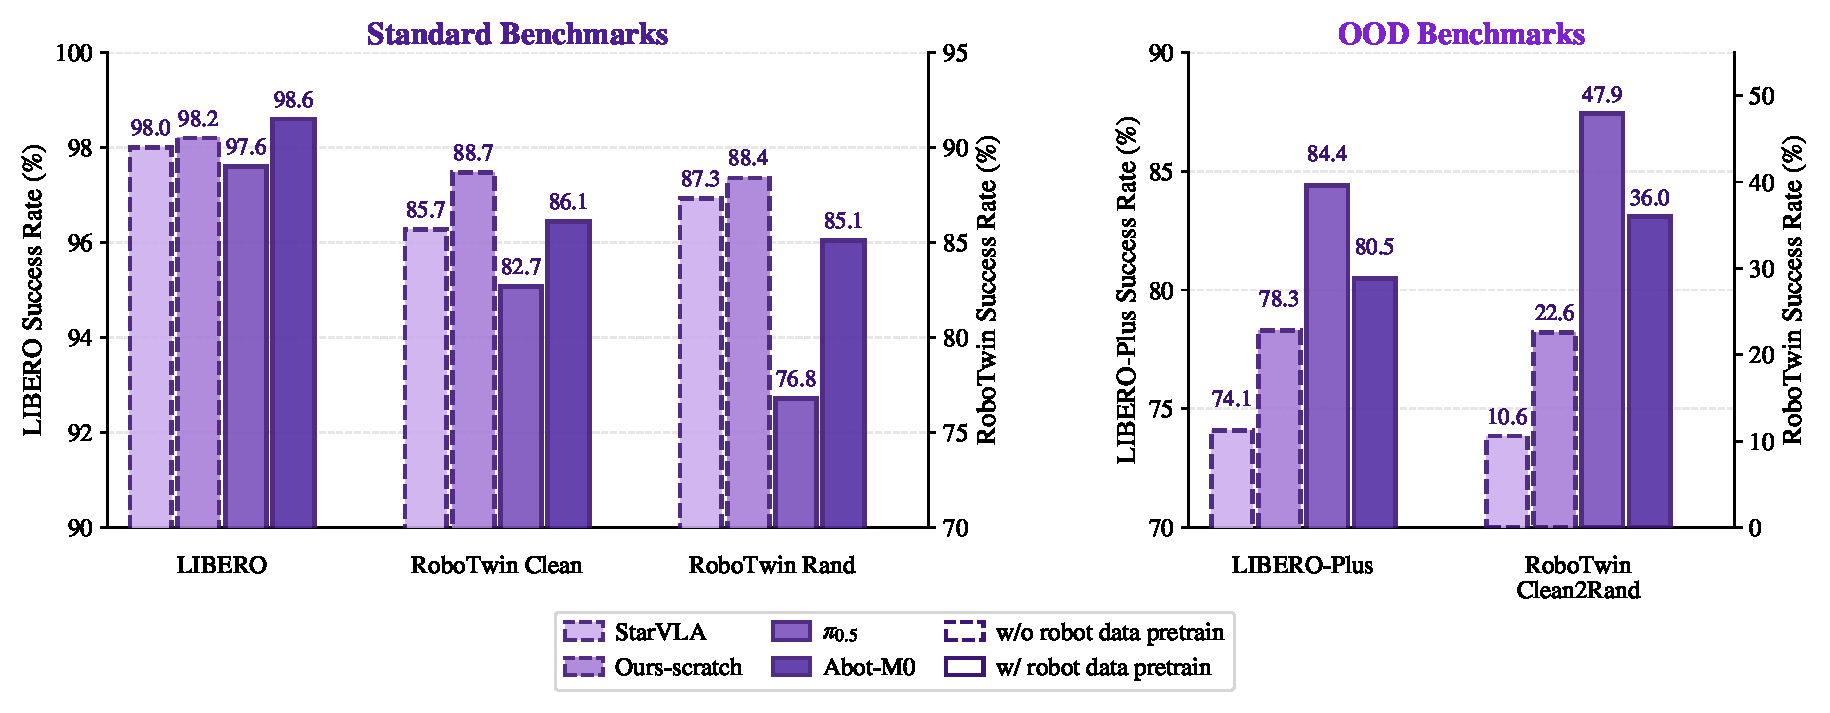
\includegraphics[width=1.0\linewidth]{figures/iid_diagnostic.pdf}
    \caption{
    \textbf{Standard in-distribution benchmarks cannot reveal whether a model benefits from large-scale robot data pretraining.}
    %\textbf{Standard benchmarks cannot distinguish pretrained from scratch models.} 
    Left: on in-distribution benchmarks (LIBERO, RoboTwin), models without large-scale robot pretraining (dashed borders) match or exceed pretrained ones. Right: on OOD benchmarks (LIBERO-Plus, RoboTwin-Clean2Rand), a clear separation emerges---pretraining provides genuine generalization that training-from-scratch cannot replicate. %OOD evaluation is the correct north star for measuring foundation model quality.
    }
    \label{fig:iid_diagnostic}
\end{figure}

% \begin{table}[!t]
% \centering
% \caption{Performance comparison across standard manipulation benchmarks. \blue{[TODO: results pending final evaluation.]}}
% \label{tab:main_results}
% \small
% \tabcolsep 4pt
% \begin{tabular}{lccc}
% \toprule
% & \textbf{LIBERO} & \multicolumn{2}{c}{\textbf{RoboTwin}} \\
% & & Easy & Hard \\
% \midrule
% $\pi_0$~\citep{black2024pi0} & 94.4 & 65.9 & 58.4 \\
% $\pi_{0.5}$~\citep{pi05} & 97.6 & 82.7 & 76.8 \\
% GR00T-N1.6~\citep{bjorck2025grootn1} & 97.2 & 47.6 & -- \\
% StarVLA~\citep{community2026starvla} & 98.0 & 85.7 & 87.3 \\
% Being-H0.7~\citep{beingh07} & 99.2 & 90.2 & 89.6 \\
% Abot-M0~\citep{yang2026abot} & 98.6 & 86.1 & 85.1 \\
% \midrule
% \ours-scratch & 98.2 &  &  \\
% \ours & \blue{99.1} & \blue{90.7} & \blue{90.6} \\
% \bottomrule
% \end{tabular}
% \end{table}

Figure~\ref{fig:iid_diagnostic} (left) reports the results. A notable pattern is that models trained from scratch---StarVLA and Ours-scratch---attain competitive or even superior results compared to well-pretrained models such as $\pi_{0.5}$ and Abot-M0 on LIBERO and RoboTwin, despite lacking large-scale robotic pretraining. This is not a coincidence but a structural property of these benchmarks. Because training and evaluation data are drawn from the same environment and task distributions, high success rates can be achieved through in-distribution pattern matching alone. Models that lack genuine generalization can perform well simply by memorizing recurring visual and behavioral patterns, and the benchmark cannot distinguish this from real capability. Prior work has further shown that fine-tuning a pretrained VLA on a benchmark's own training split yields performance comparable to training from scratch~\citep{Yan_2025_ICCV}, confirming that the pretrained prior contributes negligible transferable value under in-domain evaluation.

Figure~\ref{fig:iid_diagnostic} (right) tells a different story. On OOD benchmarks---LIBERO-Plus and RoboTwin-Clean2Rand---where evaluation conditions diverge from training, a clear separation emerges: $\pi_{0.5}$ substantially outperforms StarVLA and Ours-scratch, with the gap widening as perturbation severity increases. StarVLA collapses from 85.7\% (RoboTwin Easy, IID) to 10.6\% (RoboTwin-Clean2Rand, OOD). This confirms that OOD evaluation is the correct north star for measuring foundation model quality: it reveals the transferable structure that pretraining provides and that in-domain metrics systematically fail to capture.

The way practitioners actually use a foundation model reinforces this conclusion. A researcher or engineer deploying a VLA model does not have access to the same distribution of tasks, objects, and environments present in any benchmark. They have a handful of demonstrations collected on their own hardware, in their own workspace, for their own task. What determines whether the foundation model helps them is not its in-domain benchmark rank but how much generalizable structure it has internalized, and how efficiently that structure transfers under minimal fine-tuning on unfamiliar data. The following section therefore adopts OOD evaluation as the primary measure and reports comprehensive benchmarking results for \ours across both in-distribution and out-of-distribution settings.

\subsection{Generalization Capabilities}

The following sections evaluate \ours on a suite of out-of-distribution settings that directly measure the generalization capabilities a foundation model is expected to provide. We organize these evaluations around three axes (Figure~\ref{fig:eval_setting_overall}): task and scene generalization under controlled perturbations, instruction following with novel language and tasks, and zero-shot cross-embodiment transfer.

\begin{figure}[tb]
    \centering
    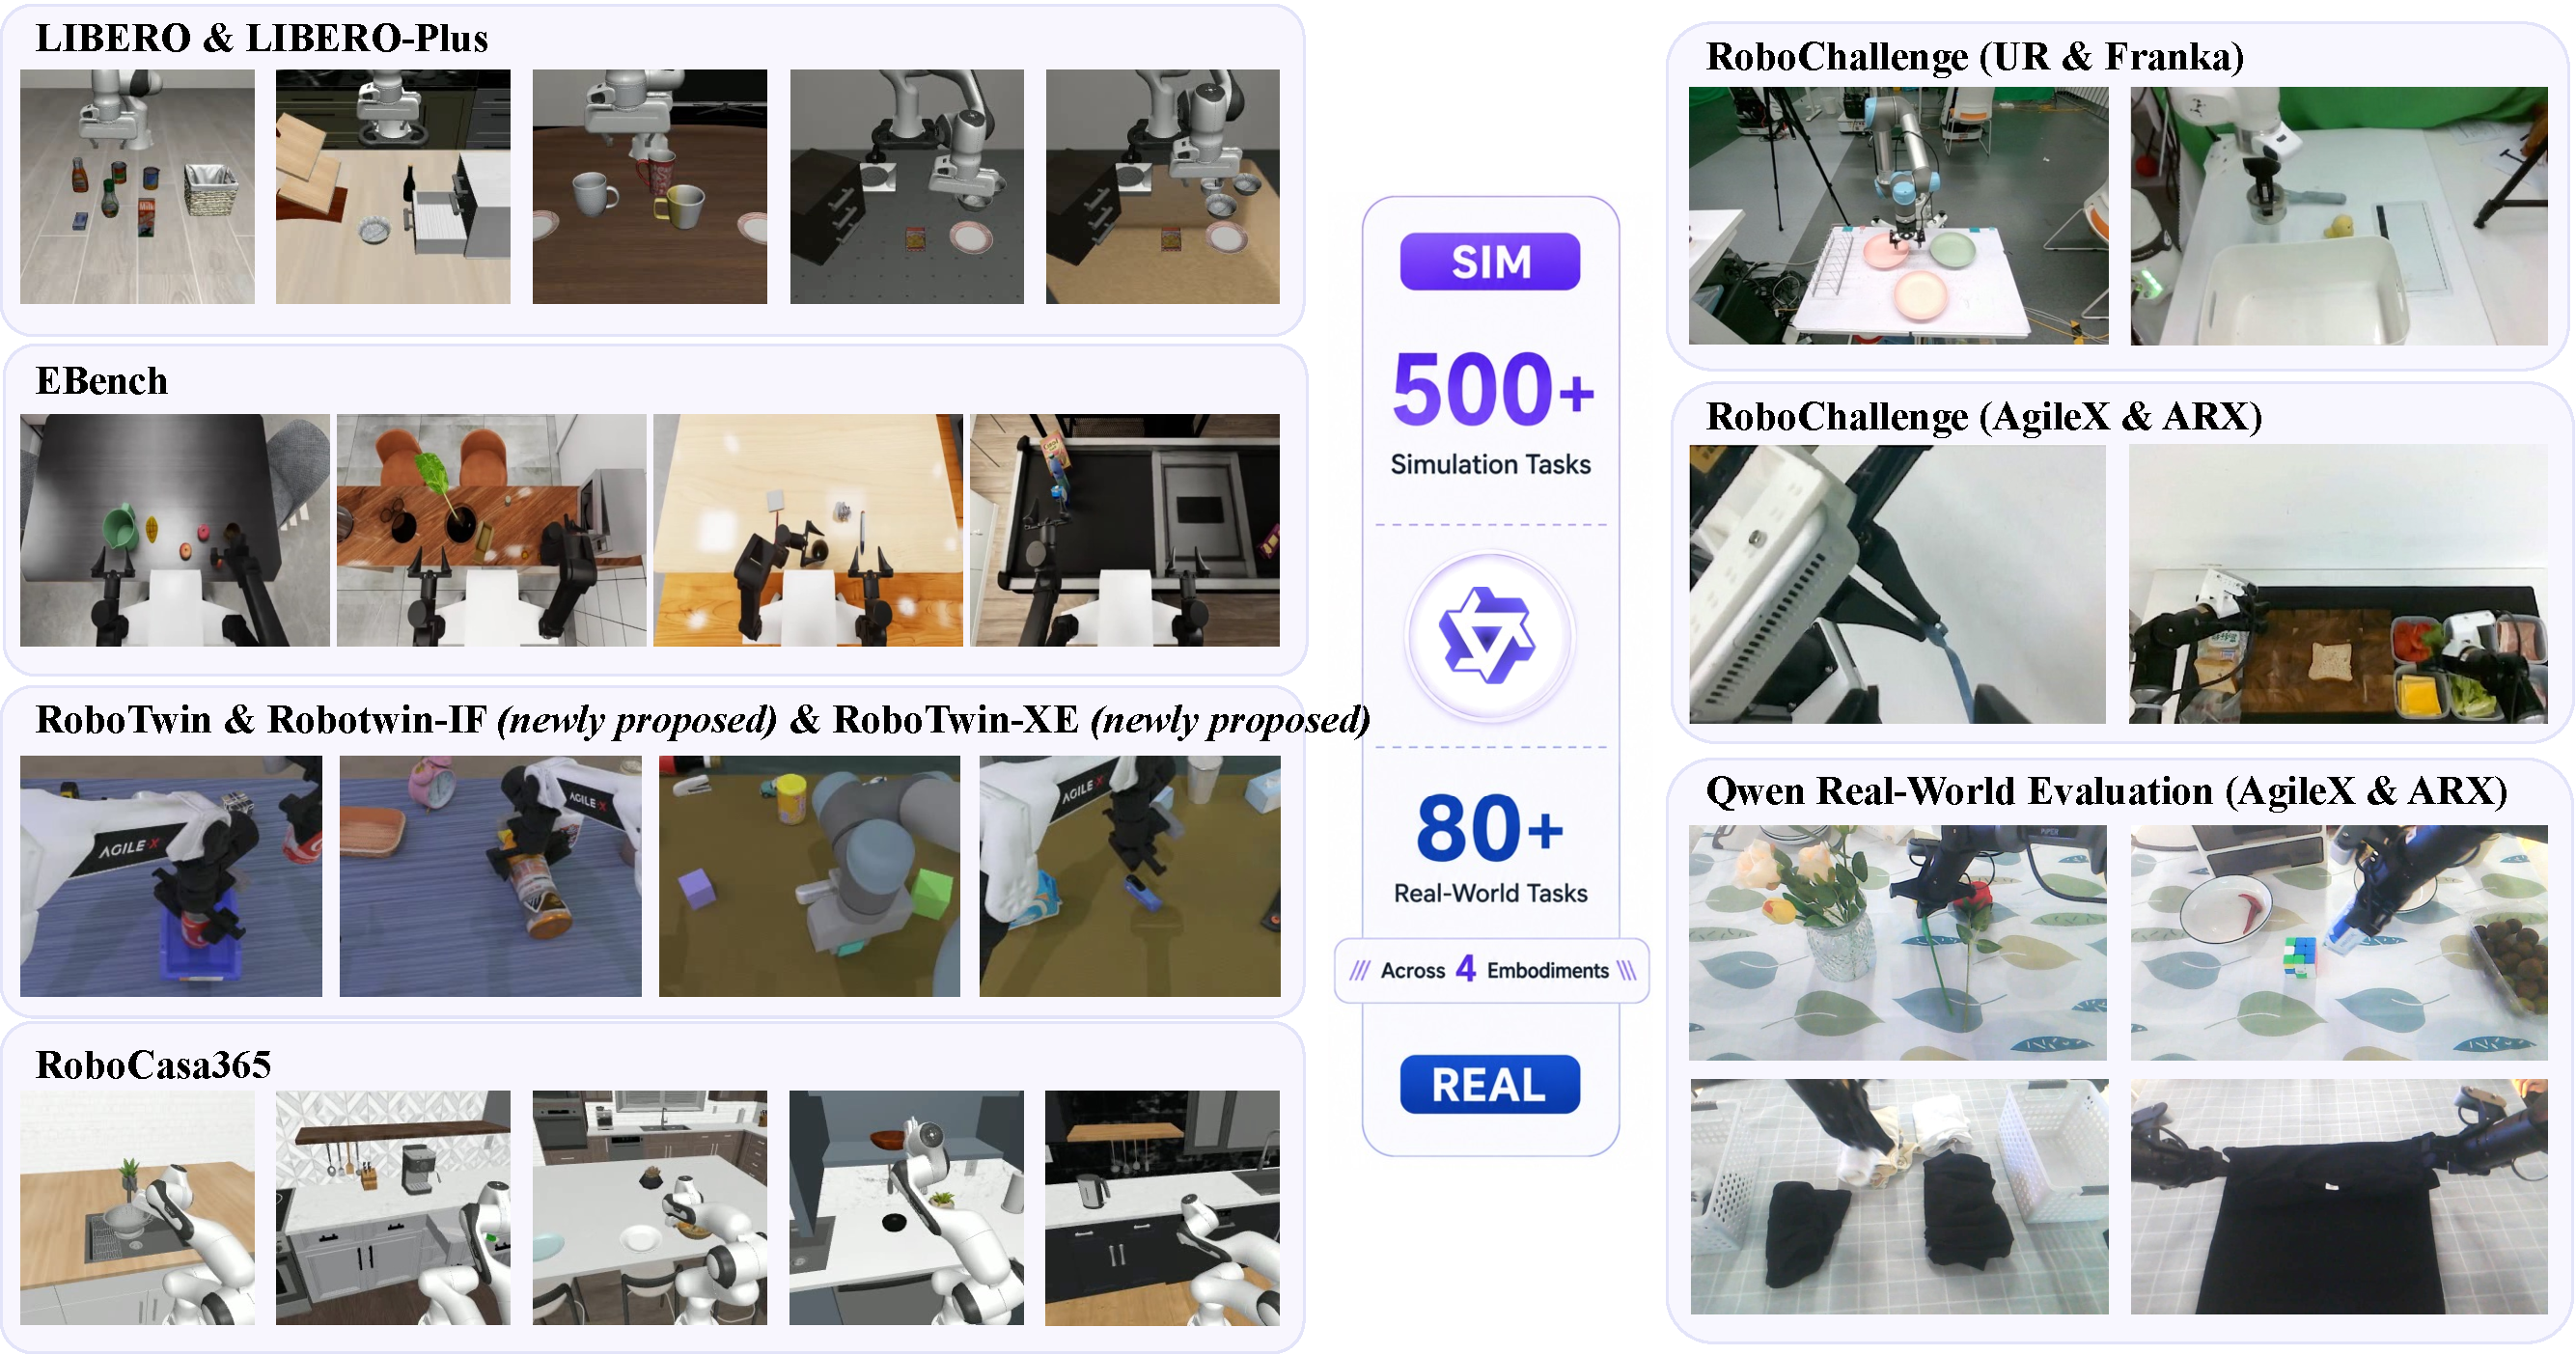
\includegraphics[width=1.0\linewidth]{figures/eval_setting_overall.pdf}
    \caption{\textbf{Evaluation settings for \ours}, spanning 500+ simulation tasks across LIBERO, LIBERO-Plus, EBench, RoboTwin, RoboTwin-IF, RoboTwin-XE, and RoboCasa365, and 80+ real-world tasks across 4 embodiments including UR, Franka, AgileX (ALOHA), and ARX.}
    \label{fig:eval_setting_overall}
\end{figure}

\subsubsection{Evaluation Protocol}
\label{sec:eval_protocol}

\paragraph{Task and Scene Generalization.}
We evaluate robustness of VLA models to visual and physical changes on four benchmarks.
\textbf{LIBERO-Plus}~\citep{fei2025liberoplus} introduces controlled perturbations along seven orthogonal dimensions on top of the original LIBERO benchmark---background textures, camera viewpoints, language instructions, lighting conditions, object layouts, robot initial states, and sensor noise---with models fine-tuned on the standard LIBERO training set and evaluated under each perturbation.
\textbf{RoboTwin-Clean2Rand} constructs an OOD evaluation protocol on top of RoboTwin~\citep{mu2025robotwin}: all models are fine-tuned exclusively on a Clean dataset with fixed white background, default lighting, no distractors, and a fixed table height, then evaluated under controlled randomizations along individual axes (background, lighting, clutter, table height) as well as a Hard setting that applies all randomizations simultaneously.
\textbf{RoboCasa365}~\citep{nasiriany2026robocasa365} provides a large-scale kitchen manipulation benchmark with three evaluation suites of increasing difficulty: Atomic (18 basic manipulation skills with diverse object and layout variations), Composite-Seen (multi-step long-horizon tasks seen during training), and Composite-Unseen (long-horizon tasks absent from the training set).
\textbf{EBench}~\citep{ebench2026} is an indoor mobile manipulation benchmark built on NVIDIA Isaac Sim, spanning 26 task types and 794 evaluation instances. The benchmark evaluates generalization along perturbation dimensions: background, instruction, object, and a mixed setting that combines all perturbations, reporting both success rate and a process score for each.

\paragraph{Instruction Following.}
Existing OOD benchmarks primarily probe robustness to visual and physical perturbations, while leaving generalization to unseen language instructions largely untested. We develop \textbf{RoboTwin-IF} (\textbf{I}nstruction \textbf{F}ollowing), a benchmark built on RoboTwin~\citep{mu2025robotwin} that systematically evaluates instruction-following capabilities across five task suites, each targeting a distinct dimension of language grounding:
%
\begin{itemize}[leftmargin=*,topsep=2pt,itemsep=1pt]
    \item \textbf{Pick-Diverse-Object}: Four objects are randomly sampled from a pool of 12 everyday items. The instruction names one object by color and noun. The robot must identify and lift the correct target among three distractors, testing \emph{target-object grounding}.
    \item \textbf{Place-Relative}: Two named objects and 1--3 distractors are on the table. The instruction specifies picking up object A and placing it in a spatial relation (``beside'' or ``on top of'') with respect to object B, testing \emph{spatial-relation understanding}.
    \item \textbf{Operate-Mic-Drawer}: A microphone and a cabinet with a functional drawer are present. The instruction specifies a multi-step bimanual sequence: open the drawer with one arm, then pick up the microphone with the other arm and place it inside. Some instructions further specify which arm performs which sub-task, testing \emph{multi-step sequencing and bimanual coordination}.
    \item \textbf{Operate-Stapler}: A stapler, a colored pad, and 1--2 distractors are on the table. The instruction specifies either pressing the stapler or moving it onto the colored pad. The pad is always present regardless of the verb, acting as a distractor in press episodes and as the placement target in move episodes, testing \emph{verb discrimination with shared scene elements}.
    \item \textbf{Operate-Tabletop}: A bell, a stapler, and 1--2 pickable objects are all present simultaneously. The instruction specifies one of three actions: ring the bell, press the stapler, or pick up a named object. Only one action is correct; the other interactive objects are distractors, testing \emph{three-way verb-and-target discrimination} in a multi-affordance scene.
\end{itemize}

\begin{figure}[tb]
    \centering
    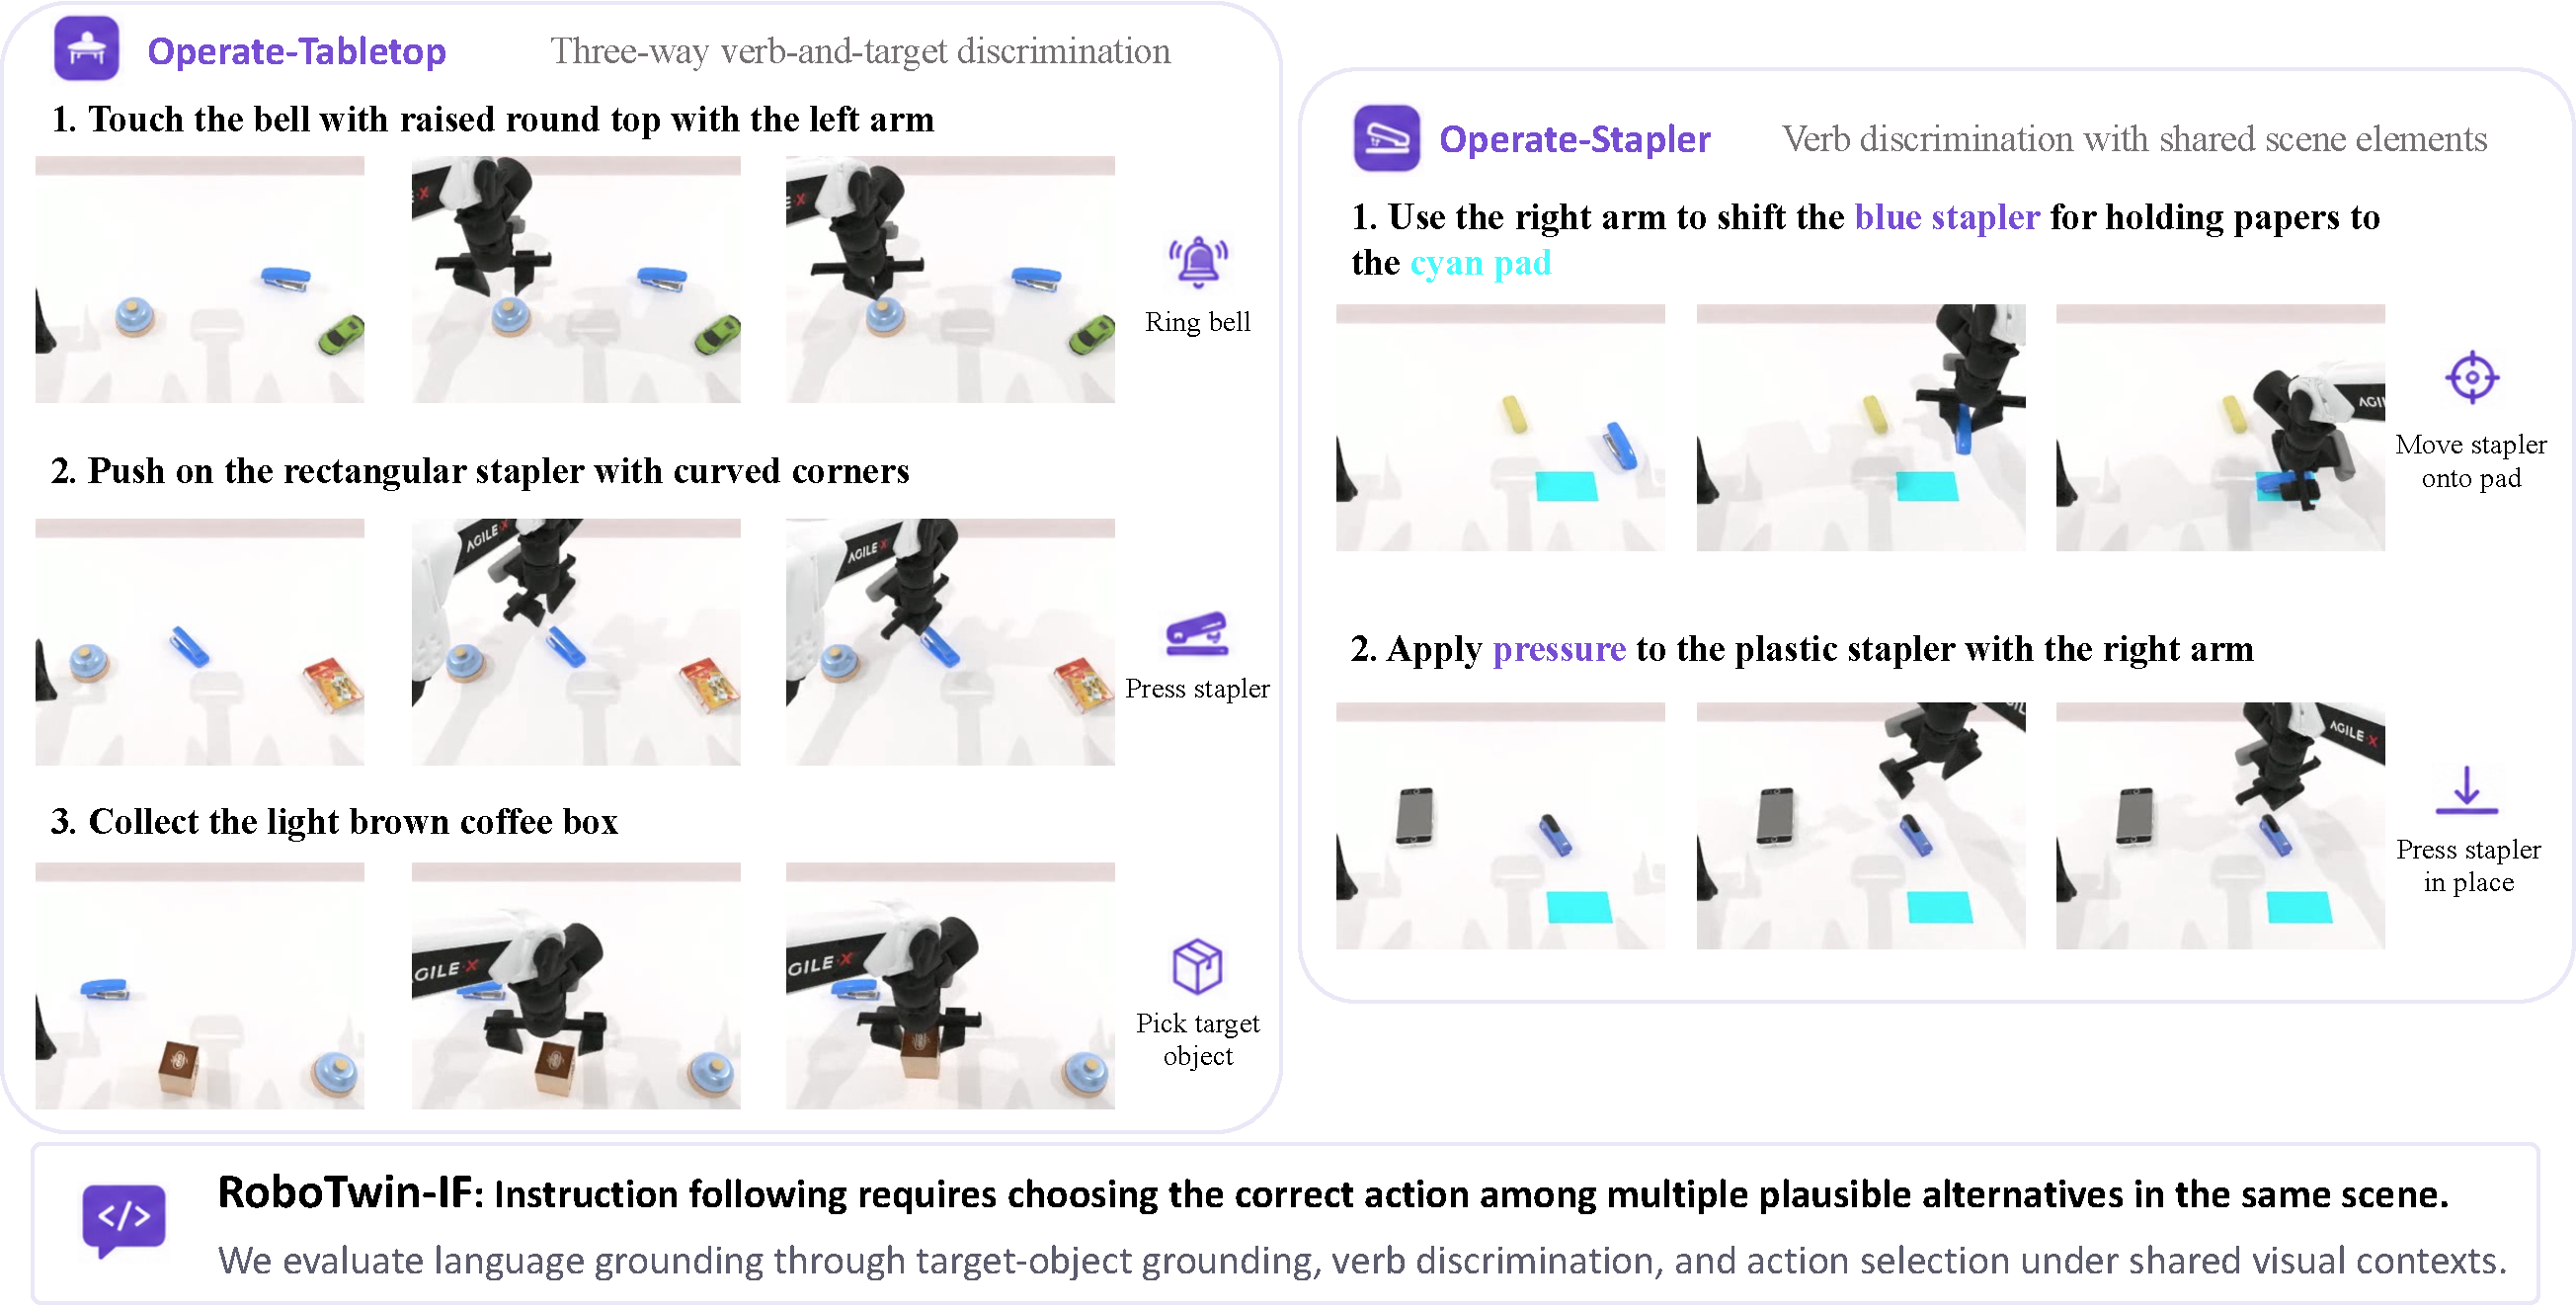
\includegraphics[width=1.0\linewidth]{figures/robotwin-IF.pdf}
    \caption{\textbf{Representative task suites from RoboTwin-IF.} Operate-Tabletop (left) requires three-way verb-and-target discrimination where a bell, stapler, and pickable objects are all present and only the instruction-specified action is correct. Operate-Stapler (right) requires verb discrimination under shared visual context, where the colored pad and stapler are always present regardless of the instructed verb. Both suites are evaluated on unseen instruction templates held out from training.}
    \label{fig:eval_robotwin_if}
\end{figure}

All models are fine-tuned exclusively on RoboTwin Clean. Each suite uses a two-tier language diversity system: ``seen'' instruction templates (used during training data collection) and ``unseen'' templates (held out for evaluation), combined with per-object description variants that further diversify noun phrases. At evaluation time, each episode is paired with a held-out unseen instruction template, ensuring zero overlap with the training distribution.

\paragraph{Cross-Embodiment Generalization.}

Camera-frame relative EEF actions express deltas in the camera coordinate frame rather than a robot-specific joint space, enabling a single policy to potentially control morphologically distinct robots without re-training. 
We develop \textbf{RoboTwin-XE}, a benchmark based on RoboTwin that evaluates zero-shot transfer to unseen robot embodiments. 
The model is fine-tuned on the RoboTwin Clean dataset and tested under the RoboTwin Hard setting, replacing the default AgileX platform with ARX-X5, UR5-WSG, and Franka Panda. 
Initial EEF poses are aligned via IK, head and wrist camera extrinsics are kept identical, and task scenes, object layouts, and perturbation seeds are shared across embodiments. 
The model must therefore generalize across two types of embodiment-specific differences: the visual appearance of the robot arm in camera observations, and kinematic differences (DOF count, joint arrangement, link lengths, and workspace geometry) that affect reachability and motion dynamics. 
The model is fine-tuned exclusively on AgileX demonstrations; no target-embodiment data is used.

%% === Summary of Results ===

\subsubsection{Summary of Results}

On standard in-distribution benchmarks, \ours achieves state-of-the-art or competitive performance (Table~\ref{tab:iid_results}) on LIBERO (99.2\%) and RoboTwin Easy/Hard (93.7\%/94.0\%). However, as argued in \cref{subsec:are_std_bench_enough}, these metrics do not reliably distinguish genuine generalization from in-distribution pattern matching. We therefore focus on OOD evaluation as the primary measure of robotic foundation model capabilities.

\begin{table}[!t]
\centering
\caption{\textbf{In-distribution benchmark results.} \ours matches or exceeds prior state-of-the-art across all standard benchmarks.}
\label{tab:iid_results}
\small
\tabcolsep 5pt
\begin{tabular}{lccc}
\toprule
& \textbf{LIBERO} & \textbf{RoboTwin-Easy} & \textbf{RoboTwin-Hard} \\
\midrule
$\pi_0$~\citep{black2024pi0} & 94.4 & 65.9 & 58.4 \\
$\pi_{0.5}$~\citep{pi05} & 97.6 & 82.7 & 76.8 \\
StarVLA~\citep{community2026starvla} & 98.0 & 85.7 & 87.3 \\
Abot-M0~\citep{yang2026abot} & 98.6 & 86.1 & 85.1 \\
Being-H0.7~\citep{beingh07} & \textbf{99.2} & 90.2 & 89.6 \\
\midrule
\ours-scratch & 98.2 & 88.7 & 88.4 \\
\ours & {99.1} & {93.4} & {92.5} \\
\ours-Context & \textbf{99.2} & \textbf{93.7} & \textbf{94.0} \\
\bottomrule
\end{tabular}
\end{table}

\begin{figure}[!t]
    \centering
    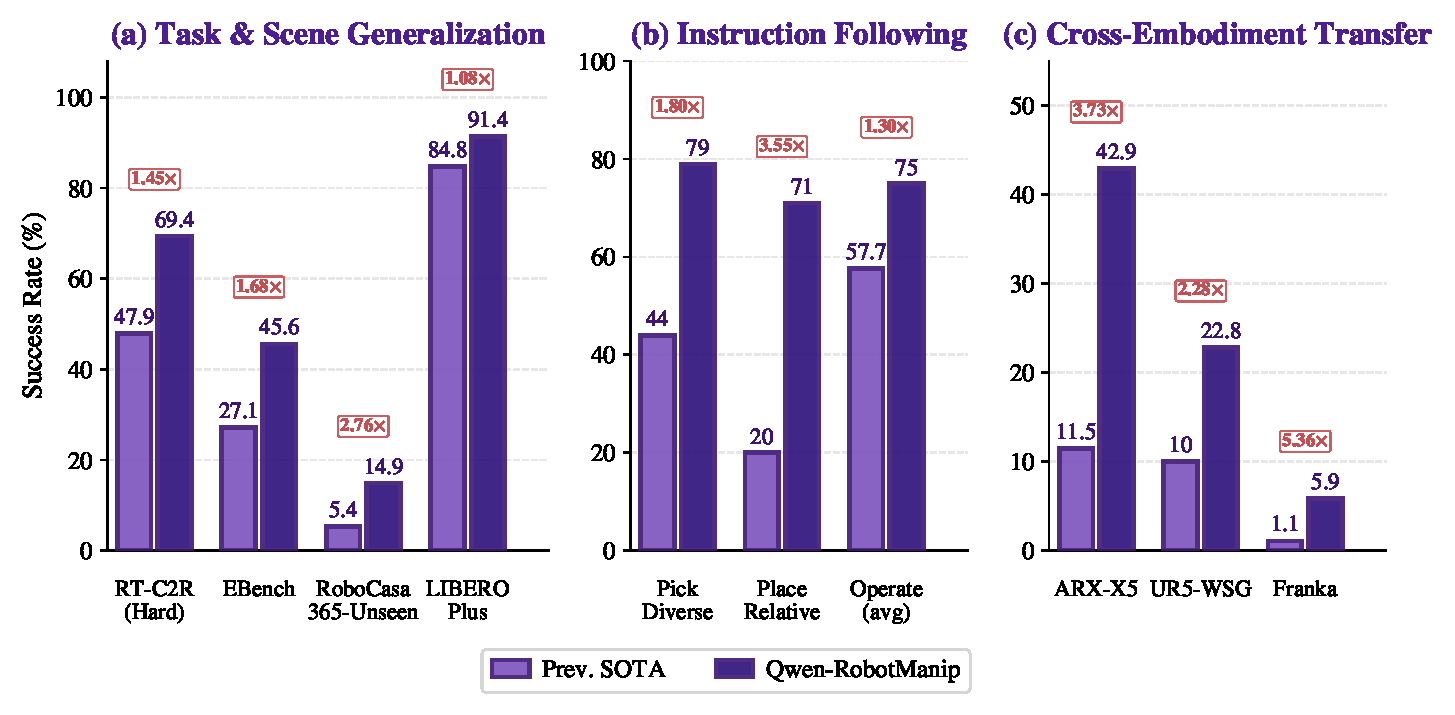
\includegraphics[width=0.9\linewidth]{figures/ood_summary.pdf}
    \caption{\textbf{OOD generalization summary.} \ours vs.\ previous state-of-the-art VLA model across three generalization axes. (a)~Task and scene generalization under controlled perturbations. (b)~Instruction following with held-out language templates. (c)~Zero-shot cross-embodiment transfer. \ours outperforms previous models on every OOD benchmark, with the gap widening on harder settings.}
    \label{fig:ood_summary}
\end{figure}

Figure \ref{fig:ood_summary} summarizes results across benchmarks evaluated under OOD settings, where \ours consistently outperforms prior state-of-the-art models by a substantial margin. \ours outperforms $\pi_{0.5}$ on all benchmarks evaluated, with the gap widening as the evaluation becomes more challenging.

On task and scene generalization, \ours surpasses $\pi_{0.5}$ by 7.0 points on LIBERO-Plus (91.4 vs.\ 84.4), by 21.5 points on the most demanding RoboTwin-C2R Hard setting (69.4 vs.\ 47.9), and by 18.5 points on EBench (45.6 vs.\ 27.1). On RoboCasa365, the advantage reaches 19.0 points (35.9 vs.\ 16.9).

On instruction following, \ours scores 72.2\% on RoboTwin-IF against 49.6\% for $\pi_{0.5}$---a large improvement of 22.6 points. This result is particularly significant because instruction following is the capability most prone to degradation during VLA training: fine-tuning a VLM on action prediction can erode the language conditioning pathway, causing the policy to collapse into a visually-triggered default behavior that ignores the instruction entirely (\cref{sec:training}). The fact that \ours maintains strong instruction following across all five RoboTwin-IF suites---including tasks requiring target-object grounding, spatial-relation understanding, and multi-way verb discrimination---indicates that the dual-stream co-training strategy and the diversity of the pretraining corpus together preserve genuine language-conditioned control.

The most revealing comparison is cross-embodiment transfer on RoboTwin-XE. When both models are trained exclusively on demonstrations collected on the AgileX ALOHA platform and evaluated zero-shot on unseen robots, \ours achieves 23.9\% using camera-frame EEF actions---3.2$\times$ the 7.5\% achieved by $\pi_{0.5}$. This gap validates our camera-frame alignment strategy for action representation: by expressing actions in the visual domain, physically similar motions become numerically proximate across morphologically distinct robots, enabling effective cross-embodiment transfer.

% A complementary signal comes from the comparison with models trained from scratch. On LIBERO-Plus, \ours-scratch scores 78.3 versus \ours's 90.1; on RoboTwin-C2R Hard, \ours-scratch collapses from 71.6 (Easy) to 22.6 (Hard)---retaining about 30\% of its Easy performance---while \ours degrades far more gracefully from 70.0 to 60.9, retaining roughly 87\% (compared to 66\% for $\pi_{0.5}$). Across benchmarks, a consistent pattern emerges: the pretrained VLM backbone already provides robustness to visual and linguistic variations (background, lighting, language), but the robot-specific structure that distinguishes genuine generalization from in-distribution memorization---spatial reasoning under novel viewpoints, robustness to novel robot states, attention to task-relevant objects amid clutter---requires the large-scale cross-embodiment pretraining that \ours provides.

A complementary signal comes from the comparison with models trained from scratch. On LIBERO-Plus, \ours-scratch scores 78.3 versus \ours's 89.0 and \ours-Context's 91.4. The gap is even more pronounced on RoboTwin-C2R, where \ours-scratch collapses from 71.6 (Easy) to 22.6 (Hard), retaining about 30\% of its Easy performance, while \ours degrades far more gracefully from 73.2 to 62.6, retaining roughly 86\% (compared to 66\% for $\pi_{0.5}$). 
A consistent pattern emerges across benchmarks. The pretrained VLM backbone already provides robustness to some of the visual and linguistic variations such as background, lighting, and language perturbations. However, the capabilities that distinguish genuine generalization from in-distribution memorization, including spatial reasoning under novel viewpoints, robustness to unseen robot states, and attention to task-relevant objects in cluttered scenes, specifically require the large-scale cross-embodiment pretraining that \ours provides.


%% === Detailed Analysis ===

\subsubsection{Detailed Analysis}

\paragraph{LIBERO-Plus.}

\begin{table}[!t]
\centering
\caption{\textbf{Out-of-distribution robustness evaluation on LIBERO-Plus across seven perturbation dimensions.}}
\label{tab:libero_plus}
\small
\tabcolsep 3pt
\begin{tabular}{lcccccccc}
\toprule
& \textbf{Camera} & \textbf{Robot} & \textbf{Language} & \textbf{Light} & \textbf{Background} & \textbf{Noise} & \textbf{Layout} & \textbf{Total} \\
\midrule
$\pi_0$~\citep{black2024pi0} & 13.8 & 6.0 & 58.8 & 85.0 & 81.4 & 79.0 & 68.9 & 53.6 \\
$\pi_{0.5}$~\citep{pi05} & 78.4 & 73.6 & 80.8 & 96.2 & 94.1 & 89.0 & 84.5 & 84.4 \\
StarVLA~\citep{community2026starvla} & 52.5 & 49.8 & \textbf{88.5} & 95.7 & 95.7 & 73.0 & 76.9 & 74.1 \\
Abot-M0~\citep{yang2026abot} & 60.4 & 67.9 & 86.4 & 96.2 & 91.6 & 86.4 & 82.6 & 80.5 \\
Cosmos-Policy~\citep{kim2026cosmos} & 75.8 & 63.3 & 81.7 & 96.5 & 88.9 & 92.7 & 82.2 & 82.2 \\
Being-H0.7~\citep{beingh07} & 82.0 & 59.0 & 82.8 & 97.8 & 90.0 & 93.5 & \textbf{88.5} & 84.8 \\
\midrule
\ours-scratch & 70.4 & 44.9 & 88.1 & 95.8 & 95.5 & 84.4 & 79.1 & 78.3  \\
%\ours & {88.4} & {74.8} & 86.9 & \textbf{99.0} & {99.3} & \textbf{98.8} & {88.3} & {90.1} \\
\ours & 87.2 & 75.5 & 85.6 & 96.6 & 97.7 & 97.7 & 87.3 & 89.0 \\
\ours-Context & \textbf{89.9} & \textbf{83.9} & {86.5} & \textbf{98.6} & \textbf{99.9} & \textbf{97.9} & {87.5} & \textbf{91.4}  \\
\bottomrule
\end{tabular}
\end{table}


Table~\ref{tab:libero_plus} reports per-dimension results. \ours achieves 89\% and \ours-Context achieves 91.4\% overall, surpassing all baselines. Beyond the aggregate score, the per-dimension breakdown reveals which capabilities benefit from large-scale robot data pretraining and which are already provided by the pretrained VLM backbone. Models without robot data pretraining (StarVLA, \ours-scratch) match most pretrained models on Language, Light, and Background perturbations, indicating that the VLM's visual and linguistic representations are inherently robust to these variations. In contrast, these same models suffer sharp degradation under Robot perturbation (49.8\% and 44.9\% vs.\ 75.5\% for \ours), where the policy must generalize across unseen initial robot states that lie outside the VLM's purview. 
\ours-Context further raises Robot perturbation robustness to 83.9\%, a +8.4 point gain over \ours, indicating that in-context history provides an implicit kinematic prior that helps the policy adapt to unfamiliar initial robot configurations within the episode.
Camera viewpoint perturbation exhibits a similar pattern (+34.7 and +16.8 over the scratch models), suggesting that robust spatial reasoning under novel camera poses requires the grounding that VLA pretraining on diverse robot setups provides, rather than the appearance-level robustness already captured by the VLM.

\begin{table}[!t]
\centering
\caption{\textbf{Out-of-distribution evaluation on RoboTwin-Clean2Rand.} Models are fine-tuned on the Clean dataset only and tested under various environmental randomizations. }
\label{tab:robotwin_e2h}
\small
\tabcolsep 3pt
\begin{tabular}{lcccccc}
\toprule
& \textbf{Easy} & \textbf{Background} & \textbf{Light} & \textbf{Clutter} & \textbf{Height} & \textbf{Hard} \\
\midrule
StarVLA~\citep{community2026starvla} & 58.1 & 27.1 & 50.9 & 24.2 & 48.4 & 10.6 \\
GR00T-N1.7~\citep{bjorck2025grootn1} & 43.6 & 40.4 & 41.9 & 27.1 & 39.0 & 20.7 \\
$\pi_{0.5}$~\citep{pi05} & {73.1} & 67.0 & 69.2 & 57.9 & 67.6 & 47.9 \\
Abot-M0~\citep{yang2026abot} & 70.7 & 56.5 & 68.8 & 46.0 & 56.3 & 36.0 \\
\midrule
\ours-scratch & 71.6 & 60.6 & {70.7} & 24.6 & 63.6 & 22.6 \\
%\ours (joint) & {70.0} & {72.3} & {68.4} & {58.7} &  {65.5} & {60.9} \\
%\ours (eef) & {69.9} & {74.8} & {67.7} & {58.3} & {67.2} & {59.5} \\
\ours (joint) & 73.2 & 74.6 & 68.4 & 61.3 & 71.0 & 62.6 \\
\ours (eef) & 74.0 & 75.8 & 70.1 & 59.8 & 69.4 & 60.8 \\
% \ours-Context (joint) & 83.9 & 80.6 & 83.2 & 70.1 & {77.4} & {65.8} \\ %12w
\ours-Context (joint) & 84.7 & \textbf{82.4} & 84.2 & \textbf{75.4} & 79.5 & \textbf{69.4} \\
% \ours-Context (eef) & \textbf{84.5} & \textbf{82.0} & \textbf{84.2} & 69.6 & \textbf{80.6} & 63.4 \\ %12w
\ours-Context (eef) & \textbf{85.0} & \textbf{82.4} & \textbf{84.7} & 66.8 & \textbf{82.9} & 64.0 \\
\bottomrule
\end{tabular}
\end{table}

\paragraph{RoboTwin-Clean2Rand.}

Table~\ref{tab:robotwin_e2h} reports results across individual and compound perturbation axes. \ours achieves the highest success rate on the Hard setting under both joint-space control (62.6\%) and end-effector control (60.8\%), with both modes performing similarly across all perturbation dimensions. Among all methods, \ours exhibits the smallest degradation from Easy to Hard, retaining roughly 86\% of its Easy performance compared to 66\% for $\pi_{0.5}$ and about 30\% for models without robot data pretraining. The Clutter perturbation further highlights this gap: \ours-scratch collapses from 71.6\% to 24.6\% when distractor objects are introduced, suggesting that the ability to attend to task-relevant objects amid clutter requires large-scale robotic data pretraining rather than in-domain fine-tuning alone. Notably, \ours scores higher under Background randomization (74.6\%) than under the Easy setting (73.2\%), likely because diverse real-world scenes in the pretraining data make randomized backgrounds more in-distribution than the plain white background of the Easy mode.
\ours-Context further amplifies these gains, reaching 84.7\% (Easy) and 69.4\% (Hard) under joint control---an improvement of +11.5 and +6.8 points over \ours. This substantial boost suggests that conditioning on intra-episode execution history provides complementary robustness to visual perturbations, as the policy can dynamically calibrate its actions based on observed outcomes rather than relying solely on the current observation.

\paragraph{RoboCasa365.}

\begin{table}[!t]
\centering
\caption{\textbf{Evaluation on RoboCasa365 across atomic and long-horizon manipulation tasks.}}
\label{tab:robocasa365}
\small
\tabcolsep 5pt
\begin{tabular}{lcccc}
\toprule
& \textbf{Atomic} & \textbf{Composite-Seen} & \textbf{Composite-Unseen} & \textbf{Total} \\
\midrule
$\pi_0$~\citep{black2024pi0} & 36.3 & 5.2  & 0.7 & 15.0 \\
$\pi_{0.5}$~\citep{pi05} & 39.6 & 7.1 & 1.2 & 16.9 \\
GR00T-N1.5~\citep{bjorck2025grootn1} & 50.7 & 14.8 & 2.7 & 23.9 \\
GR00T-N1.6~\citep{bjorck2025grootn1} & 51.1 & 9.4 & 1.7 & 21.9 \\
RLDX-1~\citep{kim2026rldx} & 63.0 & \textbf{27.5} & 5.4 & 33.2 \\
\midrule
\ours & \textbf{68.6} & 20.1 & \textbf{14.9} & \textbf{35.9} \\
\ours-Context & 63.9 & {22.6} & 11.2 & 33.8 \\
\bottomrule
\end{tabular}
\end{table}

Table~\ref{tab:robocasa365} reports results across the three evaluation suites. \ours achieves 35.9\% overall, surpassing the previous state-of-the-art RLDX-1 (33.2\%). On the Atomic suite, \ours achieves the highest score (68.6\%) among all methods, reflecting strong generalization across diverse manipulation primitives. On Composite-Unseen---where the robot must complete long-horizon tasks in OOD scenes---\ours achieves 14.9\%, nearly tripling the next-best result (5.4\% for RLDX-1), demonstrating substantially stronger out-of-distribution compositional generalization. %RLDX-1 leads on Composite-Seen (27.5 vs.\ 20.1), likely reflecting stronger in-domain long-horizon chaining on tasks seen during training.


\begin{table}[!t]
\centering
\caption{\textbf{Evaluation on EBench across three splits.} Each split reports both success rate (SR) and the EBench composite score (Score).}
\label{tab:ebench}
\small
\tabcolsep 2.5pt
\begin{tabular}{lcccccccc}
\toprule
& \multicolumn{2}{c}{\textbf{Table Top}} & \multicolumn{2}{c}{\textbf{Simple PnP}} & \multicolumn{2}{c}{\textbf{Long Horizon}} & \multicolumn{2}{c}{\textbf{Overall}} \\
\cmidrule(lr){2-3} \cmidrule(lr){4-5} \cmidrule(lr){6-7} \cmidrule(lr){8-9}
& SR & Score & SR & Score & SR & Score & SR & Score \\
\midrule
$\pi_{0}$~\citep{black2024pi0} & 15.7 & 30 & 35.0 & 39 & 17.0 & 41 & 23.6 & 37 \\
$\pi_{0.5}$~\citep{pi05} & 12.9 & 32 & 45.0 & 50 & 18.1 & 39 & 27.1 & 41 \\
X-VLA~\citep{zheng2025xvla} & 8.6 & 24 & 50.0 & 54 & 6.2 & 25 & 23.7 & 36 \\
InternVLA-A1~\citep{cai2026internvla} & 4.3 & 11 & 43.0 & 47 & 17.9 & 46 & 23.9 & 36 \\
\midrule
\ours & \textbf{50.0} & \textbf{70} & \textbf{56.5} & 60 & \textbf{29.9} & \textbf{55} & \textbf{45.6} & \textbf{60} \\
\ours-Context & 49.3 & 56 & 55.0 & \textbf{66} & 26.6 & \textbf{55} & 43.6 & 59 \\
\bottomrule
\end{tabular}
\end{table}

\begin{figure}[!t]
    \centering
    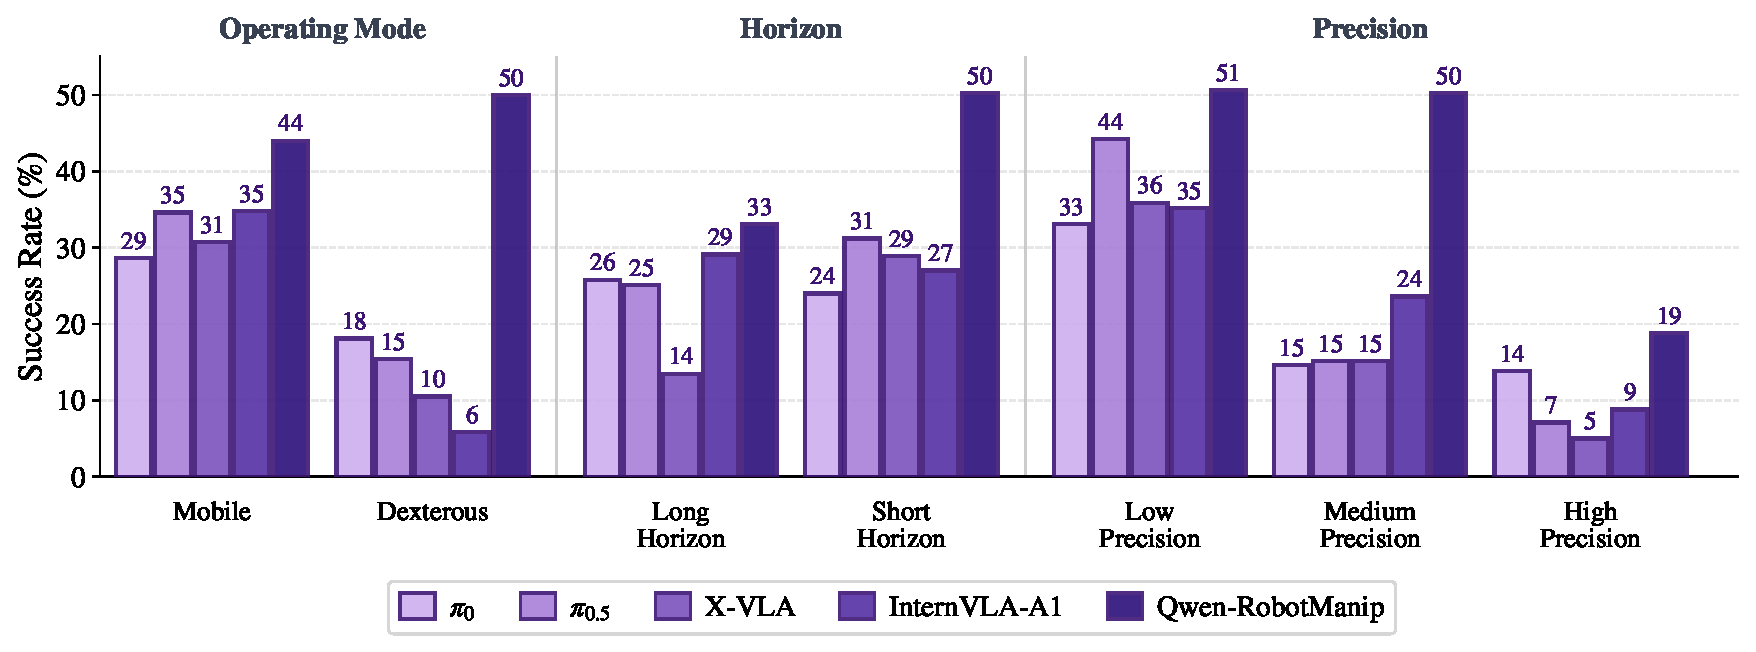
\includegraphics[width=1.0\linewidth]{figures/ebench_topline_sr.pdf}
    \caption{\textbf{EBench performance across operating mode, horizon, and precision.} }
    \label{fig:ebench_topline}
\end{figure}

\begin{figure}[!t]
    \centering
    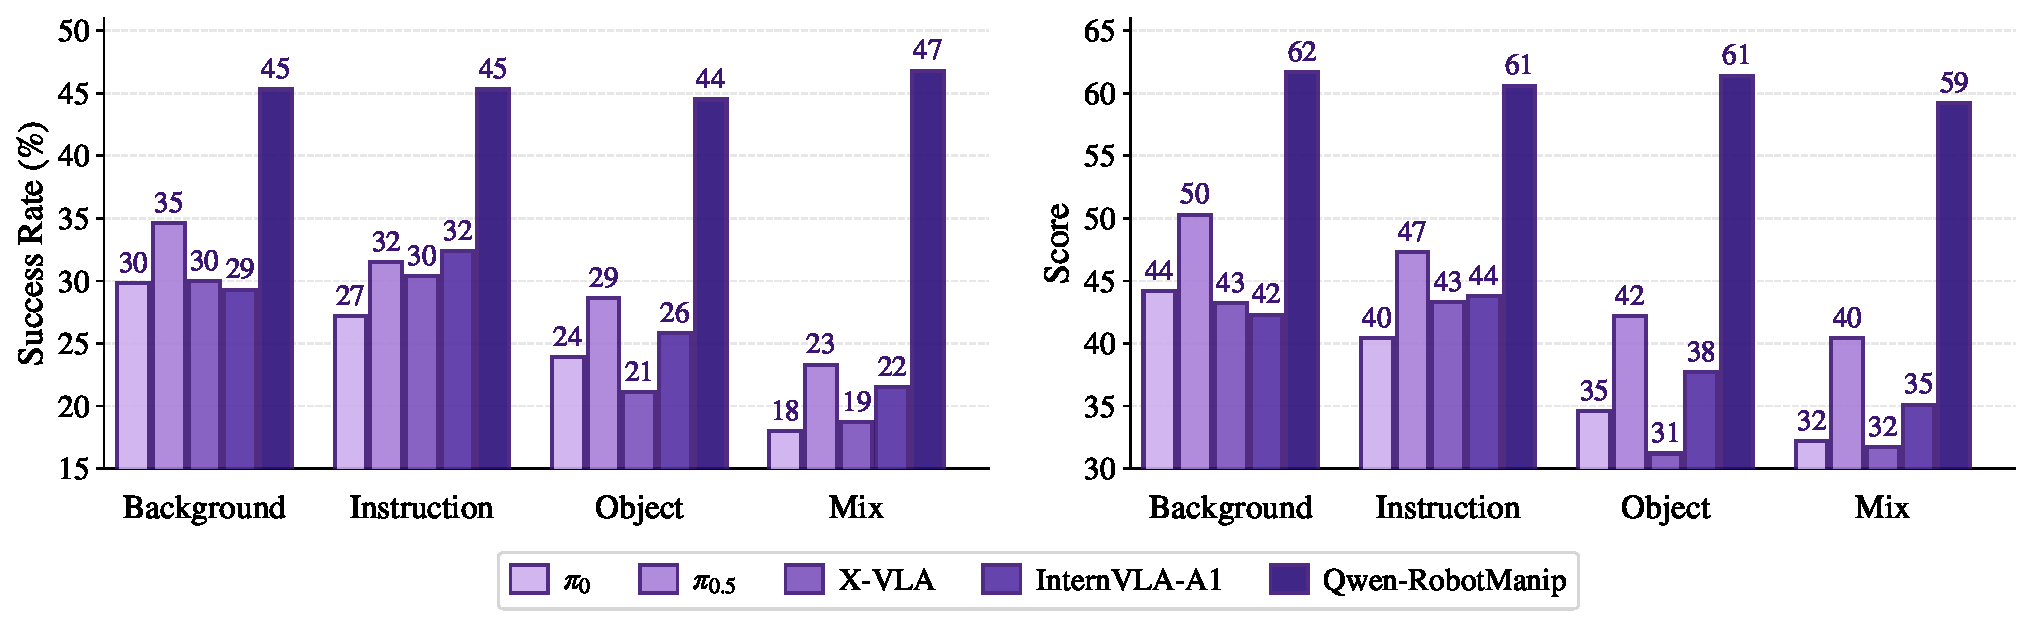
\includegraphics[width=1.0\linewidth]{figures/ebench.pdf}
    \caption{\textbf{Per-dimension generalization breakdown on EBench.} }
    \label{fig:ebench_generalize}
\end{figure}

\paragraph{EBench.}
Table~\ref{tab:ebench} and Figure~\ref{fig:ebench_topline} report the results on EBench~\citep{ebench2026}, an Isaac Sim-based indoor manipulation benchmark that evaluates 26 task types on a dual-arm mobile platform (Lift2 + R5a) across three splits: dexterous tabletop tasks (Table Top), pick-and-place with mobile manipulation (Simple PnP), and extended multi-step sequences (Long Horizon). 
\ours achieves 45.6\% overall success rate and a composite score of 60, outperforming $\pi_{0.5}$ (27.1\% / 41) and all other baselines by a large margin across every split.

The gains are most striking on the dexterous split. 
On Table Top, \ours achieves 50.0\% SR and a score of 70, nearly quadrupling $\pi_{0.5}$'s success rate (12.9\%) and more than doubling its score (32). 
On Simple PnP, \ours leads at 56.5\% SR while the next-best baseline is X-VLA at 50.0\%.
On Long Horizon, which requires mobile manipulation over extended sequences, \ours reaches 29.9\% SR and a score of 55, improving over $\pi_{0.5}$ by +11.8 SR and +16 score.
Figure~\ref{fig:ebench_topline} further breaks down performance by operating mode, horizon length, and precision level, showing consistent advantages across all seven dimensions.

The per-dimension generalization breakdown (Figure~\ref{fig:ebench_generalize}) further confirms robustness to distribution shift. 
As perturbation complexity increases, baseline performance degrades substantially---$\pi_{0.5}$'s SR drops from 34.6 under Background to 23.3 under Mix (a 33\% decline). 
In contrast, \ours remains remarkably stable across all dimensions (SR 44.5--46.8), with virtually no degradation under compounded perturbations.
The gap over the next-best method widens from Background (+10.7 SR) and Instruction (+12.9), to Object (+15.9) and Mix (+23.5). 
Under the most demanding Mix condition---where background, instruction, and object perturbations are applied simultaneously---\ours achieves 46.8\%, even surpassing its own Background score (45.3\%), whereas $\pi_{0.5}$ drops from 34.6 to 23.3 ($-$33\%). 
This near-uniform performance under diverse distribution shifts demonstrates strong generalization robustness.



% Table~\ref{tab:ebench} and Figure~\ref{fig:ebench} report the results. \ours achieves 38.0\% success rate and a composite score of 51, substantially outperforming $\pi_{0.5}$ (27.1\% / 41) and all other baselines. The improvement is particularly notable given that EBench tests mobile manipulation with a humanoid embodiment---a setting absent from most VLA pretraining corpora---confirming that \ours's alignment framework transfers to embodiments beyond those seen during training.


% Old commented-out table (superseded by tab:ebench above)

\paragraph{RoboTwin-IF.}


\begin{table}[!t]
\centering
\caption{\textbf{Instruction-following evaluation on RoboTwin-IF.} Models are fine-tuned on RoboTwin Clean dataset and evaluated with held-out unseen instruction templates. }
\label{tab:robotwin_if}
\small
\tabcolsep 2.5pt
\begin{tabular}{lcccccc}
\toprule
& \textbf{Pick-Diverse} & \textbf{Place-Rel.}  & \textbf{Ope.-Mic-Dr.} & \textbf{Ope.-Stapler} & \textbf{Ope.-Table} & \textbf{Average} \\
\midrule
StarVLA~\citep{community2026starvla} & 11 & 13  & 0 & 49 & 74 & 29.4 \\
GR00T-N1.7~\citep{bjorck2025grootn1} & 20 & 17  & 0 & 14 & 32 & 16.6 \\
%Abot-M0~\citep{yang2026abot} & -- & --  & -- & -- & -- & -- \\
%Being-H0.7~\citep{beingh07} & -- & --  & -- & -- & -- & -- \\
$\pi_{0.5}$~\citep{pi05} & 44 & 20 & 15 & \textbf{92} & 66   & 49.6 \\
\midrule
% \ours & 76 & 61 & \textbf{44} & 89 & 88 & 71.6 \\
\ours & \textbf{79} & 57 & \textbf{42} & 90 & \textbf{93} & \textbf{72.2} \\
% \ours-Context (joint) & 73 & 62 & 39 & 88 & 87 & 69.8 \\
\ours-Context & {77} & \textbf{71} & 33 & 89 & {90} & {72.0} \\ % eef
% \ours + VLM Co-Train & 79 & 45 & 40 & 90 & 89 & 68.6 \\
% \ours + Mix Pre-Train & 74 & 60 & 45 & 88 & 88 & 71 \\
\bottomrule
\end{tabular}
\end{table}

Table~\ref{tab:robotwin_if} reports per-suite results. \ours achieves 72.2\% average versus $\pi_{0.5}$'s 49.6\%, a gap of 22.6 points. The improvement happens on four of five suites, with large gains on Pick-Diverse (+35), Place-Relative (+37), Operated-Mic-Drawer (+27), and Operated-Tabletop (+27)---tasks where the instruction must be parsed to determine the correct action among multiple plausible alternatives in the same scene. This comprehensive advantage confirms that \ours has learned genuine language-conditioned control rather than relying on visual shortcuts.


\paragraph{Zero-Shot Cross-Embodiment.}

Table~\ref{tab:cross_embodiment} reports zero-shot transfer for both joint-space and camera-frame relative EEF representations on RoboTwin-XE. 
Joint-space control transfers poorly: joint configurations are robot-specific, so actions meaningful for one morphology produce near-random behavior on another---UR5 and Franka stay below 5\% for both methods. 
Switching to camera-frame EEF dramatically improves transfer: \ours reaches 42.9\% on ARX, 22.8\% on UR5 ($5.6\times$ the joint result), and 5.9\% on Franka, for a cross-embodiment average of 23.9\%. 
This confirms that the camera-frame representation successfully abstracts away morphological differences, allowing the policy to reason in shared Cartesian space. 
Our model consistently outperforms $\pi_{0.5}$ in both action spaces, with the largest gap on UR5 (22.8 vs.\ 10.0). The performance gradient (ARX $>$ UR5 $>$ Franka) correlates with visual and kinematic similarity to the training embodiment: ARX-X5 shares a visually similar 6-DOF form factor and similar reach to AgileX, UR5 differs in appearance and joint arrangement but has a similar workspace, while Franka's distinct 7-DOF morphology and larger reach present the greatest mismatch.

\begin{figure}[!t]
\centering
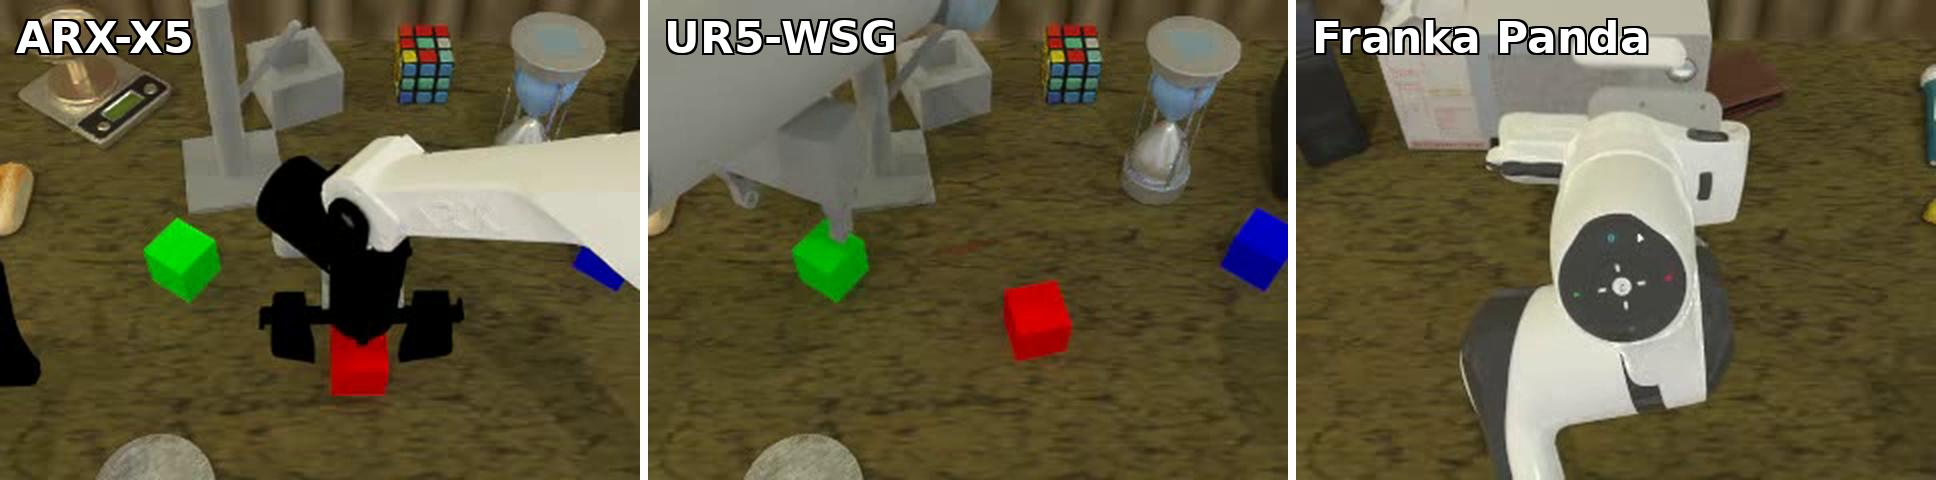
\includegraphics[width=0.8\columnwidth]{figures/fig_cross_embodiment.pdf}
\caption{\textbf{Zero-shot cross-embodiment evaluation on RoboTwin-XE.} 
% The same policy (trained on Aloha-Agilex) deployed on three unseen embodiments under randomized conditions. 
Left: ARX-X5. Middle: UR5-WSG. Right: Franka Panda.
}
\label{fig:cross_embodiment}
\end{figure}

\begin{table}[!t]
\centering
\caption{\textbf{Zero-shot performance on RoboTwin-XE}, where models are trained on RoboTwin Clean and tested on Hard settings with unseen robot embodiments. 
% Models are trained exclusively on Aloha-Agilex demonstrations and evaluated on unseen embodiments without any target-embodiment data.
}
\label{tab:cross_embodiment}
\small
\tabcolsep 5pt
\begin{tabular}{lcccc}
\toprule
& \textbf{ARX-X5} & \textbf{UR5-WSG} & \textbf{Franka Panda} & \textbf{Total} \\
\midrule
$\pi_{0.5}$ (joint)~\citep{pi05} & 24.6 & 2.2  & 0.9 & 9.2 \\
$\pi_{0.5}$ (eef)~\citep{pi05} & 11.5 & 10.0 & 1.1 & 7.5 \\
\midrule
\ours (joint) & 37.6 & 4.1 & 1.8 & 14.5 \\
\ours (eef) & \textbf{42.9} & \textbf{22.8} & \textbf{5.9} & \textbf{23.9} \\
\bottomrule
\end{tabular}
\end{table}


% \subsection{Are Standard Benchmarks Enough?}

% We evaluate \ours on robotic manipulation benchmarks that span a diverse range of embodiments and task types, and compare against several recent VLA models~\cite{black2024pi0, bjorck2025grootn1, community2026starvla, pi05}. 
% We begin with LIBERO~\citep{liu2023libero} and RoboTwin~\citep{mu2025robotwin}, two standard benchmarks that are widely used for VLA evaluation.
% LIBERO~\citep{liu2023libero} comprises four single-arm tabletop manipulation suites across 130 combinations of tasks and scenes. 
% %RoboCasa-GR1~\citep{nasiriany2024robocasa} features 24 upper-body tabletop manipulation tasks on the Fourier GR1 humanoid platform. 
% RoboTwin~\citep{mu2025robotwin} presents 50 dual-arm manipulation tasks in easy and hard modes, requiring adaptation to varied backgrounds, objects, and spatial layouts.

% \begin{figure}[!h]
%     \centering
%     \includegraphics[width=1.0\linewidth]{figures/iid_vs_ood2.pdf}
%     \caption{Results on standard in-distribution benchmarks (left) and OOD benchmarks (right). Dashed borders indicate models without large-scale robot data pretraining.}
%     \label{fig:iid_vs_ood}
% \end{figure}

% \begin{table}[!t]
% \centering
% \caption{Performance comparison across standard manipulation benchmarks. \blue{[TODO: results pending final evaluation.]}}
% \label{tab:main_results}
% \small
% \tabcolsep 4pt
% \begin{tabular}{lccc}
% \toprule
% & \textbf{LIBERO} & \multicolumn{2}{c}{\textbf{RoboTwin}} \\
% & & Easy & Hard \\
% \midrule
% $\pi_0$~\citep{black2024pi0} & 94.4 & 65.9 & 58.4 \\
% $\pi_{0.5}$~\citep{pi05} & 97.6 & 82.7 & 76.8 \\
% GR00T-N1.6~\citep{bjorck2025grootn1} & 97.2 & 47.6 & -- \\
% StarVLA~\citep{community2026starvla} & 98.0 & 85.7 & 87.3 \\
% Being-H0.7~\citep{beingh07} & 99.2 & 90.2 & 89.6 \\
% Abot-M0~\citep{yang2026abot} & 98.6 & 86.1 & 85.1 \\
% \midrule
% \ours-scratch & 98.2 &  &  \\
% \ours & \blue{99.1} & \blue{90.7} & \blue{90.6} \\
% \bottomrule
% \end{tabular}
% \end{table}

% Figure~\ref{fig:iid_vs_ood} reports the results. \ours achieves state-of-the-art performance across all benchmarks, surpassing strong VLA baselines including $\pi_{0.5}$.

% These results, however, tell an incomplete story. A notable pattern in our experiments is that \ours-scratch and StarVLA also attain competitive results on LIBERO and RoboTwin, often approaching the best-performing models despite being trained from scratch without pretraining on large-scale robotic manipulation data. This is not a coincidence but a structural property of these benchmarks. Because training and evaluation data are drawn from the same environment and task distributions, high success rates can be achieved through in-distribution pattern matching alone. Models that lack genuine generalization can perform well simply by memorizing recurring visual and behavioral patterns, and the benchmark cannot distinguish this from real capability. Prior work has further shown that fine-tuning a pretrained VLA on a benchmark's own training split yields performance comparable to training from scratch~\citep{Yan_2025_ICCV}, confirming that the pretrained prior contributes negligible transferable value under in-domain evaluation.

% The way practitioners actually use a foundation model exposes this gap sharply. A researcher or engineer who downloads \ours does not have access to the same distribution of tasks, objects, and environments present in any benchmark. They have a handful of demonstrations collected on their own hardware, in their own workspace, for their own task. What determines whether the foundation model helps them is not its in-domain benchmark rank but how much generalizable structure it has internalized, and how efficiently that structure transfers under minimal fine-tuning on unfamiliar data. This is the setting that matters, and it is precisely the setting that standard benchmarks are not designed to probe. The following section therefore evaluates \ours on a suite of OOD settings that more faithfully reflect real deployment conditions and more directly measure the generalization capability that a foundation model is expected to provide.


% \subsection{Generalization Capabilities}

% \begin{figure}[tb]
%     \centering
%     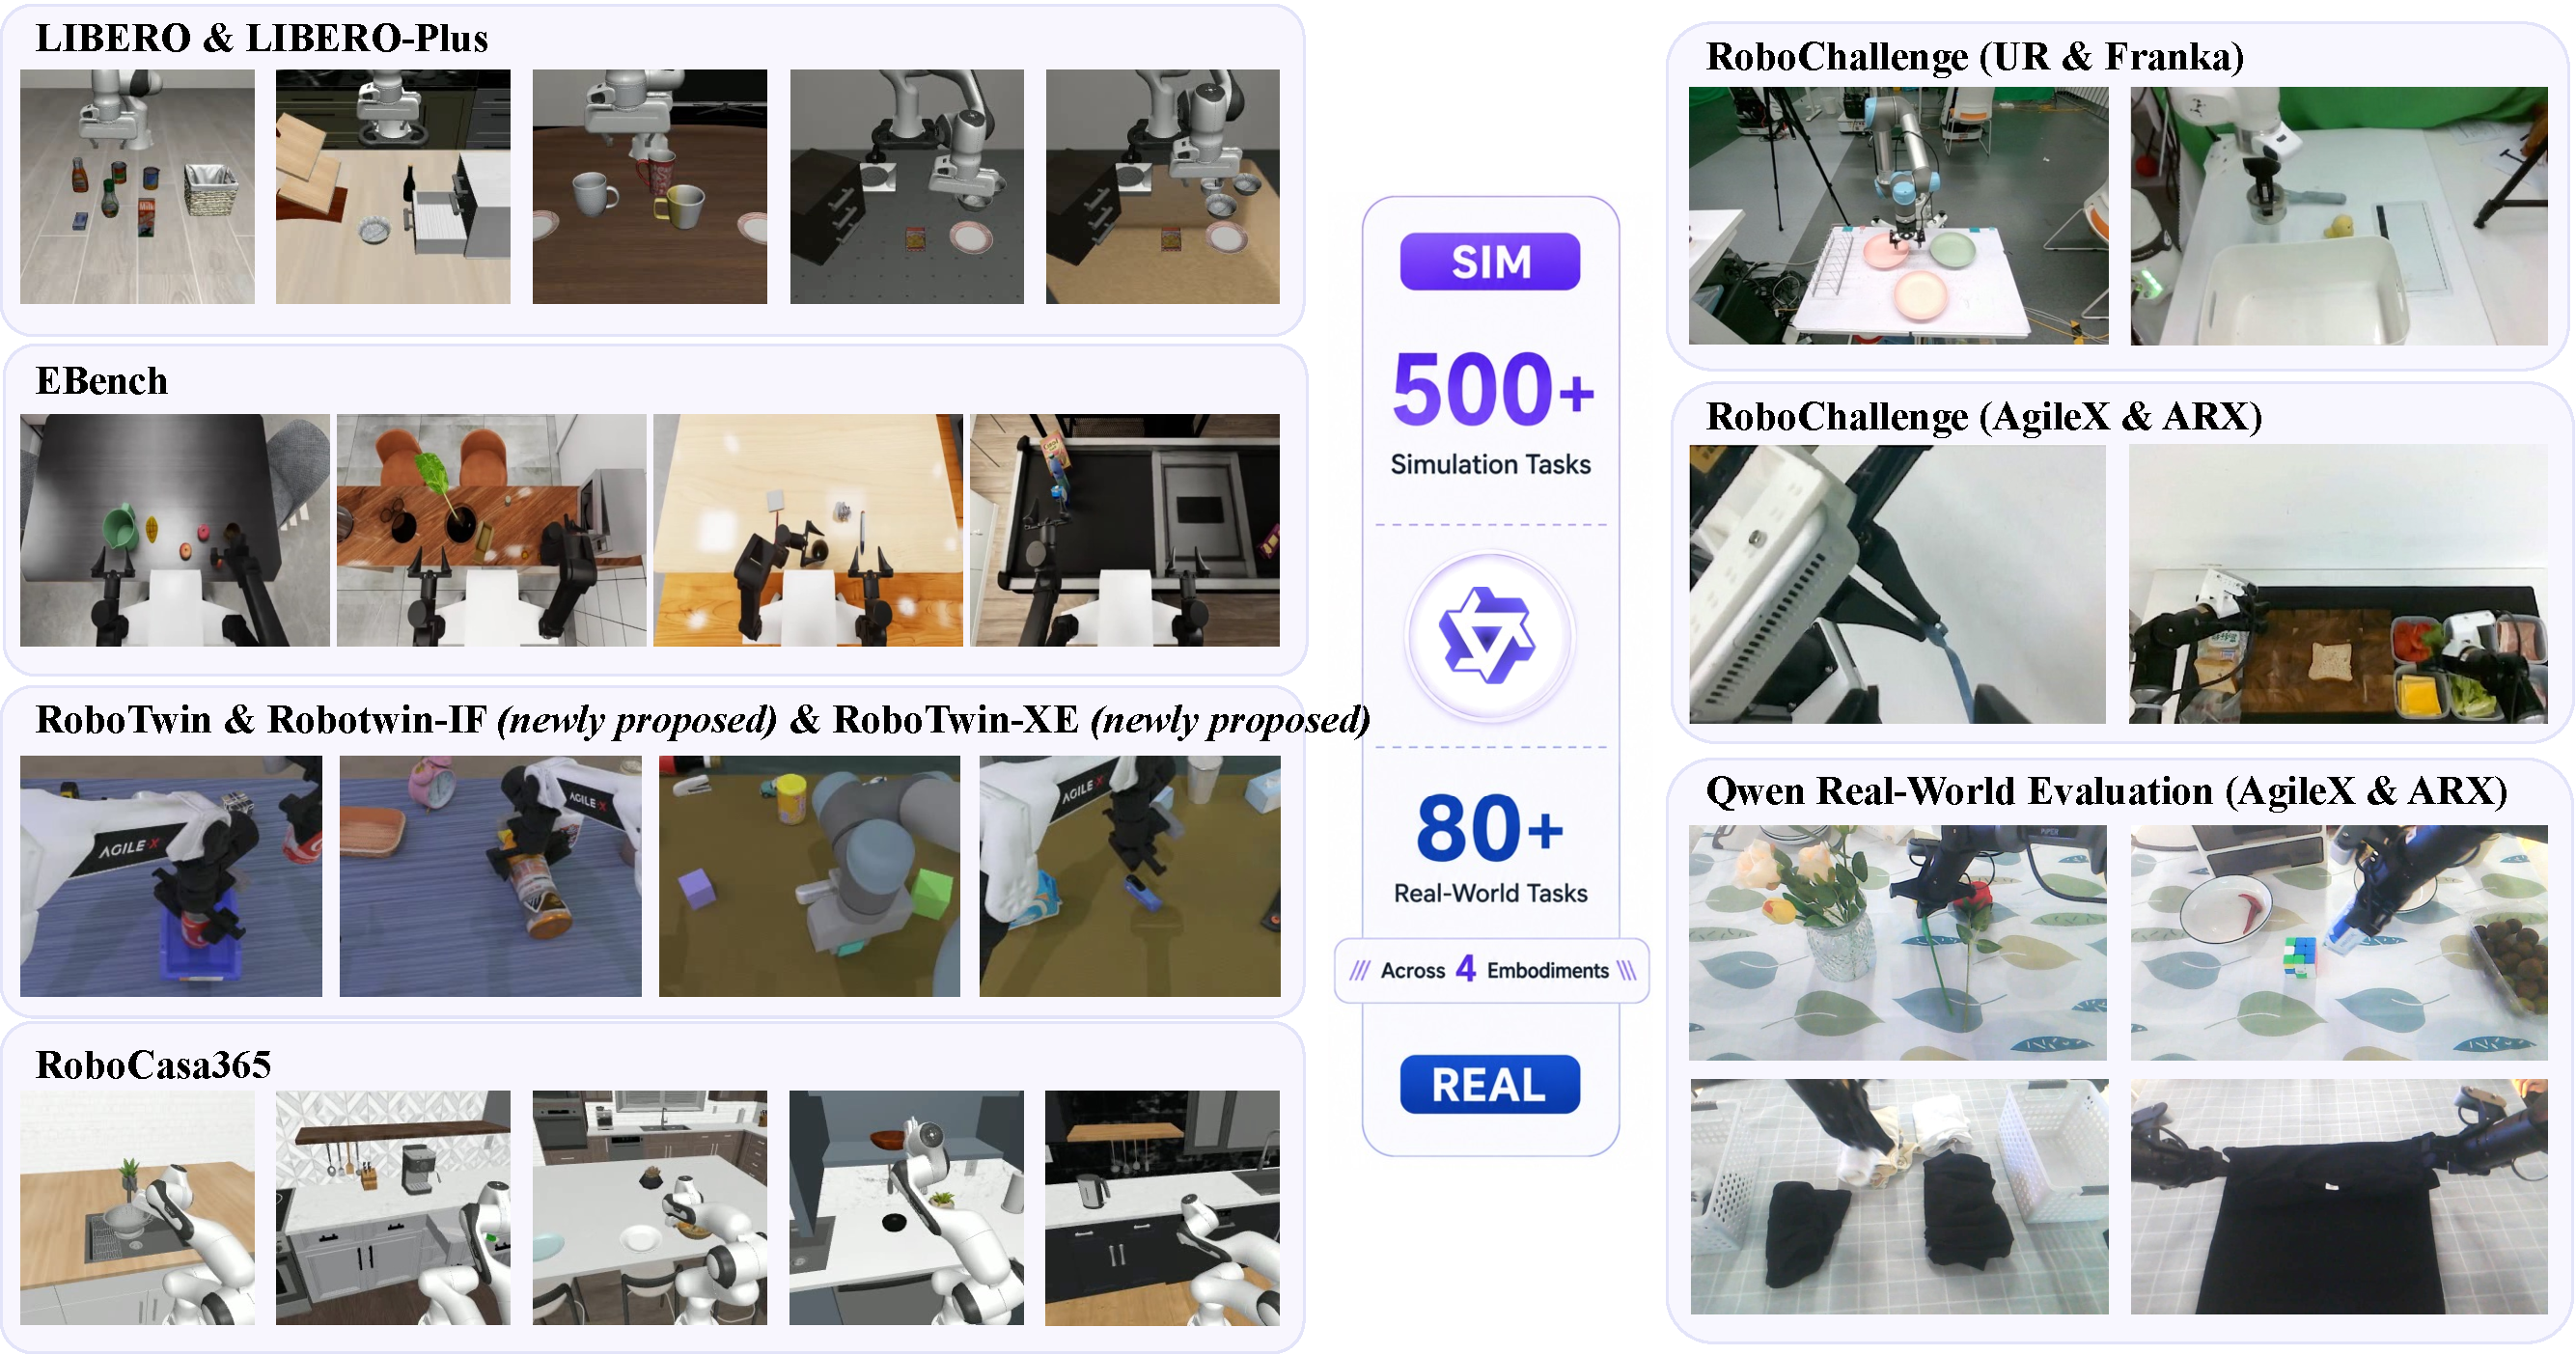
\includegraphics[width=1.0\linewidth]{figures/eval_setting_overall.pdf}
%     \caption{\textbf{Evaluation settings for \ours}, spanning 500+ simulation tasks across LIBERO, LIBERO-Plus, E-Bench, RoboTwin, RoboTwin-IF, and RoboCasa, and 80+ real-world tasks across 4 embodiments including UR, Franka, AgileX (ALOHA), and ARX. Simulation benchmarks cover both standard in-distribution settings and OOD generalization challenges. Real-robot evaluations span competitive settings from RoboChallenge and proprietary tabletop and clothes-manipulation scenarios, collectively providing a comprehensive assessment of generalization from controlled benchmarks to open-world deployment.}
%     \label{fig:eval_setting_overall}
% \end{figure}

% \subsubsection{Task and Scene Generalization}

%The results in \cref{tab:main_results} show that even models without large-scale pre-training can achieve competitive performance on standard benchmarks, because training and test distributions are tightly aligned. 
% To rigorously evaluate whether \ours has learned genuinely generalizable manipulation capabilities, we conduct a comprehensive out-of-distribution evaluation across multiple benchmarks, probing various axes of generalization.

% \paragraph{LIBERO-Plus.}
% LIBERO-Plus~\citep{fei2025liberoplus} provides a systematic robustness analysis framework for VLA models by introducing controlled perturbations along seven orthogonal dimensions on top of the original LIBERO benchmark: background textures, camera viewpoints, language instructions, lighting conditions, object layouts, robot initial states, and sensor noise.
% Models are fine-tuned on the standard LIBERO training set and evaluated under each perturbation.

% \begin{table}[!t]
% \centering
% \caption{Out-of-distribution robustness evaluation on LIBERO-Plus across seven perturbation dimensions.}
% \label{tab:libero_plus}
% \small
% \tabcolsep 3pt
% \begin{tabular}{lcccccccc}
% \toprule
% & \textbf{Camera} & \textbf{Robot} & \textbf{Language} & \textbf{Light} & \textbf{Background} & \textbf{Noise} & \textbf{Layout} & \textbf{Total} \\
% \midrule
% $\pi_0$~\citep{black2024pi0} & 13.8 & 6.0 & 58.8 & 85.0 & 81.4 & 79.0 & 68.9 & 53.6 \\
% $\pi_{0.5}$~\citep{pi05} & 78.4 & 73.6 & 80.8 & 96.2 & 94.1 & 89.0 & 84.5 & 84.4 \\
% StarVLA~\citep{community2026starvla} & 52.5 & 49.8 & \textbf{88.5} & 95.7 & 95.7 & 73.0 & 76.9 & 74.1 \\
% Abot-M0~\citep{yang2026abot} & 60.4 & 67.9 & 86.4 & 96.2 & 91.6 & 86.4 & 82.6 & 80.5 \\
% Being-H0.7~\citep{beingh07} & -- & -- & -- & -- & -- & -- & -- & 82.1 \\
% \midrule
% \ours-scratch & 70.4 & 44.9 & 88.1 & 95.8 & 95.5 & 84.4 & 79.1 & 78.3  \\
% \ours & \textbf{88.4} & \textbf{74.8} & 86.9 & \textbf{99.0} & \textbf{99.3} & \textbf{98.8} & \textbf{88.3} & \textbf{90.1} \\
% \ours-Context & {83.6} & {72.2} & {86.5} & {95.7} & {97.5} & {93.8} & {86.7} & {87.2}  \\
% \bottomrule
% \end{tabular}
% \end{table}

% Table~\ref{tab:libero_plus} reports the results. \ours achieves 90.1\% overall, surpassing all baselines. Beyond the overall score, the per-dimension breakdown reveals which capabilities benefit from large-scale robot data pretraining and which are already provided by the pretrained VLM backbone. Models without robot data pretraining (StarVLA, \ours-scratch) match most pretrained models on Language, Light, and Background perturbations, indicating that the VLM's visual and linguistic representations are inherently robust to these variations. In contrast, these same models suffer a sharp degradation under Robot perturbation (49.8\% and 44.9\% vs.\ 74.8\% for \ours), where the policy must generalize across unseen initial robot states that lie outside the VLM's purview. Camera viewpoint perturbation exhibits a similar pattern, suggesting that robust spatial reasoning under novel camera poses requires the grounding that VLA pretraining on diverse robot setups provides, rather than the appearance-level robustness already captured by the VLM.

% \paragraph{RoboTwin-Clean2Rand.}
% To evaluate generalization along orthogonal dimensions on bimanual manipulation tasks, we construct an out-of-distribution evaluation protocol on top of RoboTwin~\citep{mu2025robotwin}.
% All models are fine-tuned exclusively on the Clean dataset, which contains a fixed white background, default lighting, no distractor objects, and a fixed table height.
% At evaluation time, we introduce controlled randomizations along individual axes, as well as the Hard setting that applies all randomizations simultaneously.

% \begin{table}[!t]
% \centering
% \caption{Out-of-distribution evaluation on RoboTwin-Clean2Rand. Models are fine-tuned on the Clean dataset only and tested under various environmental randomizations. }
% \label{tab:robotwin_e2h_main}
% \small
% \tabcolsep 3pt
% \begin{tabular}{lcccccc}
% \toprule
% & \textbf{Easy} & \textbf{Background} & \textbf{Light} & \textbf{Clutter} & \textbf{Height} & \textbf{Hard} \\
% \midrule
% StarVLA~\citep{community2026starvla} & 58.1 & 27.1 & 50.9 & 24.2 & 48.4 & 10.6 \\
% GR00T-N1.7~\citep{bjorck2025grootn1} & 43.6 & 40.4 & 41.9 & 27.1 & 39.0 & 20.7 \\
% $\pi_{0.5}$~\citep{pi05} & \textbf{73.1} & 67.0 & 69.2 & 57.9 & \textbf{67.6} & 47.9 \\
% \midrule
% \ours-scratch & 71.6 & 60.6 & \textbf{70.7} & 24.6 & 63.6 & 22.6 \\
% \ours (joint) & {70.0} & {72.3} & {68.4} & \textbf{58.7} &  {65.5} & \textbf{60.9} \\
% \ours (eef) & {69.9} & \textbf{74.8} & {67.7} & {58.3} & {67.2} & {59.5} \\
% \ours-Context & -- & -- & -- & -- & -- & -- \\
% \bottomrule
% \end{tabular}
% \end{table}

% Table~\ref{tab:robotwin_e2h_main} reports the results. \ours achieves the highest success rate on the Hard setting under both joint-space control (60.9\%) and end-effector control (59.5\%), with both modes performing similarly across all perturbation dimensions. Among all methods, \ours also exhibits the smallest degradation from Easy to Hard, retaining roughly 87\% of its Easy performance compared to 66\% for $\pi_{0.5}$ and about 30\% for models without robot data pretraining. The Clutter perturbation further highlights this gap: \ours trained from scratch collapses from 71.6\% to 24.6\% when distractor objects are introduced, suggesting that the ability to attend to task-relevant objects amid clutter requires large-scale robotic data pretraining rather than in-domain fine-tuning alone. Notably, \ours scores higher under Background randomization (72.3\%) than under the Easy setting (70.0\%), likely because diverse real-world scenes in the pretraining data make randomized backgrounds more in-distribution than the plain white background of the Easy mode.


% \paragraph{RoboCasa365.}
% RoboCasa365~\citep{nasiriany2026robocasa365} provides a large-scale kitchen manipulation benchmark with three evaluation suites of increasing difficulty.
% The Atomic suite evaluates 18 basic manipulation skills with diverse object and layout variations.
% The Composite-Seen suite chains multiple atomic skills into long-horizon tasks.
% The Composite-Unseen suite evaluates long-horizon tasks not seen in the training dataset.

% \begin{table}[!t]
% \centering
% \caption{Evaluation on RoboCasa365 across atomic and long-horizon manipulation tasks. }
% \label{tab:robocasa365}
% \small
% \tabcolsep 5pt
% \begin{tabular}{lcccc}
% \toprule
% & \textbf{Atomic} & \textbf{Composite-Seen} & \textbf{Composite-Unseen} & \textbf{Total} \\
% \midrule
% $\pi_0$~\citep{black2024pi0} & 36.3 & 5.2  & 0.7 & 15.0 \\
% $\pi_{0.5}$~\citep{pi05} & 39.6 & 7.1 & 1.2 & 16.9 \\
% GR00T-N1.5~\citep{bjorck2025grootn1} & 43.0 & 9.6 & 4.4 & 20.0 \\
% RLDX-1~\citep{kim2026rldx} & 63.0 & \textbf{27.5} & 5.4 & 33.2 \\
% \midrule
% \ours & \textbf{68.6} & 20.1 & \textbf{14.9} & \textbf{35.9} \\
% \ours-Context & -- & -- & -- & -- \\
% \bottomrule
% \end{tabular}
% \end{table}

% Table~\ref{tab:robocasa365} reports the results. \ours achieves 35.9\% overall, surpassing the previous state-of-the-art RLDX-1 (33.2\%). On the Atomic suite, \ours achieves the highest score among all methods, reflecting strong generalization across diverse manipulation primitives. On Composite-Unseen, where the robot should complete long-horizon tasks in OOD scenes, \ours achieves 14.9\%, nearly tripling the next-best result (5.4\%), demonstrating substantially stronger out-of-distribution compositional generalization.


% \paragraph{MolmoSpaces.}
% MolmoSpaces~\citep{kim2026molmospaces} evaluates manipulation policies trained on the DROID~\citep{khazatsky2024droid} dataset in simulation across diverse unseen scenes, probing cross-scene generalization and the ability to handle the long tail of everyday spatial and object variations.

% \begin{table}[!t]
% \centering
% \caption{Evaluation on MolmoSpaces task suites. \blue{[TODO: results pending final evaluation.]}}
% \label{tab:molmospaces}
% \small
% \tabcolsep 5pt
% \begin{tabular}{lccccc}
% \toprule
% & \textbf{Pick} & \textbf{Pick\&Place} & \textbf{Open} & \textbf{Close} & \textbf{Total} \\
% \midrule
% $\pi_{0}$-DROID~\citep{black2024pi0} & 16.2 & 12.5 & 11.0 & 53.1 & 23.2 \\
% $\pi_{0.5}$-DROID~\citep{pi05} & 36.4 & 13.6 & 22.7 & 65.1 & 34.5 \\
% MolmoAct2-DROID~\citep{fang2026molmoact2} & 43.7 & 26.7 & 9.5 & 70.8 & 37.7 \\
% \midrule
% \ours & -- & -- & -- & -- & -- \\
% \ours-Context & -- & -- & -- & -- & -- \\
% \bottomrule
% \end{tabular}
% \end{table}

% \blue{[TODO: the analysis should be revised after results are completed.]}
% Table~\ref{tab:molmospaces} reports the results.

% \paragraph{EBench.}
% EBench~\citep{ebench2026} is an indoor mobile manipulation benchmark built on NVIDIA Isaac Sim, spanning 26 task types and 794 evaluation instances. The benchmark evaluates generalization along perturbation dimensions: background, instruction, object, and a mixed setting that combines all perturbations, reporting both success rate and a process score for each.

% \begin{table}[!t]
% \centering
% \caption{Evaluation on EBench across three splits. Each split reports both success rate (SR) and the EBench composite score (Score).}
% \label{tab:ebench}
% \small
% \tabcolsep 2.5pt
% \begin{tabular}{lcccccccc}
% \toprule
% & \multicolumn{2}{c}{\textbf{Table Top}} & \multicolumn{2}{c}{\textbf{Simple PnP}} & \multicolumn{2}{c}{\textbf{Long Horizon}} & \multicolumn{2}{c}{\textbf{Overall}} \\
% \cmidrule(lr){2-3} \cmidrule(lr){4-5} \cmidrule(lr){6-7} \cmidrule(lr){8-9}
% & SR & Score & SR & Score & SR & Score & SR & Score \\
% \midrule
% $\pi_{0}$~\citep{black2024pi0} & 15.7 & 30 & 35.0 & 39 & 17.0 & 41 & 23.6 & 37 \\
% $\pi_{0.5}$~\citep{pi05} & 12.9 & 32 & 45.0 & 50 & 18.1 & 39 & 27.1 & 41 \\
% X-VLA~\citep{zheng2025xvla} & 8.6 & 24 & 50.0 & 54 & 6.2 & 25 & 23.7 & 35 \\
% InternVLA-A1~\citep{cai2026internvla} & 4.3 & 11 & 43.0 & 47 & 17.9 & 46 & 23.9 & 36 \\
% \midrule
% \ours & -- & -- & -- & -- & -- & -- & 38.0 & 51 \\
% % \ours-Context & -- & -- & -- & -- & -- & -- & -- & -- \\
% \bottomrule
% \end{tabular}
% \end{table}

% \begin{figure}[!t]
%     \centering
%     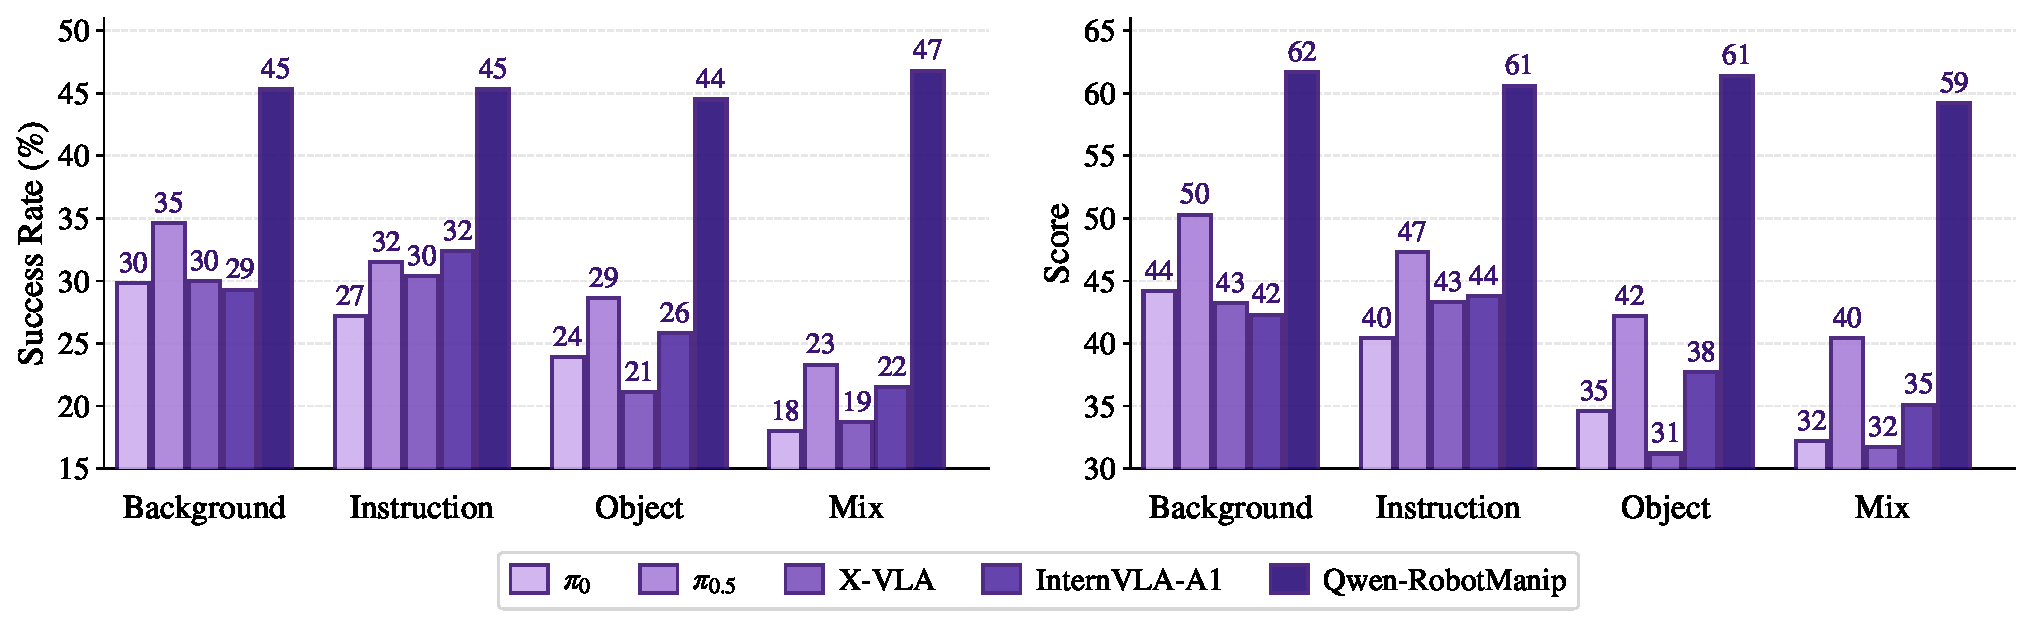
\includegraphics[width=1.0\linewidth]{figures/ebench.jpg}
%     \caption{\textbf{Ebench Generalist Leaderboard.} }
%     \label{fig:ebench}
% \end{figure}

% As shown in the official EBench Generalist Leaderboard (Figure~\ref{fig:ebench}), \ours substantially outperforms all previous models in both success rate and composite score across all generalization dimensions, establishing a new state of the art on this benchmark.


% \subsubsection{Instruction-Following}

% Existing OOD evaluation benchmarks for VLA models primarily probe robustness to visual and physical perturbations, while leaving generalization to unseen language instructions largely untested.
% In practice, a deployed VLA model will encounter instruction phrasings, verb choices, and compositional structures that differ substantially from its training distribution. A model that achieves high task success by pattern-matching visual cues while ignoring the instruction has not learned genuine language-conditioned control (\cref{sec:training}).

% To address this gap, we develop \textbf{RoboTwin-IF} (\textbf{I}nstruction \textbf{F}ollowing), a benchmark built on the RoboTwin~\citep{mu2025robotwin} simulation platform that systematically evaluates instruction-following capabilities across five task suites, each targeting a distinct dimension of language grounding.
% All models are fine-tuned exclusively on the RoboTwin Clean training set. At evaluation time, each episode is paired with a held-out unseen instruction template, ensuring that the test instructions have no overlap with the training distribution.

% The five suites are designed as follows:

% \begin{itemize}[leftmargin=*,topsep=2pt,itemsep=1pt]
%     \item \textbf{Pick-Diverse-Object}: Four objects are randomly sampled from a pool of 12 everyday items and placed on the table. The instruction names one object by color and noun. The robot must identify and lift the correct target among three distractors, testing \emph{target-object grounding}.

%     \item \textbf{Place-Relative}: Two named objects and 1--3 distractors are on the table. The instruction specifies picking up object A and placing it in a spatial relation (``beside'' or ``on top of'') with respect to object B, testing \emph{spatial-relation understanding}.

%     % \item \textbf{Operated-Mic}: A microphone and a cabinet (visual distractor) are on the table. The instruction specifies one of two manipulation verbs: pick-and-place (lift and set back down) or drag (slide along the surface). The same object is present in every episode; only the verb differs, testing \emph{action-type discrimination on a single object}.

%     \item \textbf{Operated-Mic-Drawer}: A microphone and a cabinet with a functional drawer are present. The instruction specifies a multi-step bimanual sequence: open the drawer with one arm, then pick up the microphone with the other arm and place it inside. Some instructions further specify which arm performs which sub-task, testing \emph{multi-step sequencing and bimanual coordination}.

%     \item \textbf{Operated-Stapler}: A stapler, a colored pad, and 1--2 distractors are on the table. The instruction specifies either pressing the stapler or moving it onto the colored pad. The pad is always present regardless of the verb, acting as a distractor in press episodes and as the placement target in move episodes, testing \emph{verb discrimination with shared scene elements}.

%     \item \textbf{Operated-Tabletop}: A bell, a stapler, and 1--2 pickable objects are all present simultaneously. The instruction specifies one of three actions: ring the bell, press the stapler, or pick up a named object. Only one action is correct; the other interactive objects are distractors, testing \emph{three-way verb-and-target discrimination} in a multi-affordance scene.
% \end{itemize}

% Each suite uses a two-tier language diversity system: ``seen'' instruction templates (used during training data collection) and ``unseen'' templates (held out for evaluation), combined with per-object description variants that further diversify noun phrases. This design ensures that even if the model memorizes training-time phrasings, it must generalize to novel linguistic expressions of the same intent.

% \begin{table}[!t]
% \centering
% \caption{Instruction-following evaluation on RoboTwin-IF. Models are fine-tuned on RoboTwin Clean dataset and evaluated with held-out unseen instruction templates. \blue{[TODO: results pending final evaluation.]}}
% \label{tab:robotwin_if}
% \small
% \tabcolsep 2.5pt
% \begin{tabular}{lcccccc}
% \toprule
% & \textbf{Pick-Diverse} & \textbf{Place-Rel.}  & \textbf{Ope.-Mic-Dr.} & \textbf{Ope.-Stapler} & \textbf{Ope.-Table} & \textbf{Average} \\
% \midrule
% StarVLA~\citep{community2026starvla} & 11 & --  & -- & -- & -- & \orange{haoqi} \\
% GR00T-N1.7~\citep{bjorck2025grootn1} & 20 & 17  & -- & -- & -- & \orange{haoqi} \\
% Abot-M0~\citep{yang2026abot} & -- & --  & -- & -- & -- & -- \\
% Being-H0.7~\citep{beingh07} & -- & --  & -- & -- & -- & -- \\
% $\pi_{0.5}$~\citep{pi05} & 33 & 22 & 5 & 83 & 62   & 41.0 \\
% \midrule
% \ours & 76 & 61 & 44 & 89 & 88 & 71.6 \\
% \ours-Context & -- & -- & -- & -- & -- & -- \\
% % \ours + VLM Co-Train & 79 & 45 & 40 & 90 & 89 & 68.6 \\
% % \ours + Mix Pre-Train & 74 & 60 & 45 & 88 & 88 & 71 \\
% \bottomrule
% \end{tabular}
% \end{table}

% \blue{[TODO: the analysis should be revised after results are completed.]}
% Table~\ref{tab:robotwin_if} reports the results.

% \begin{figure}[!t]
% \centering
% 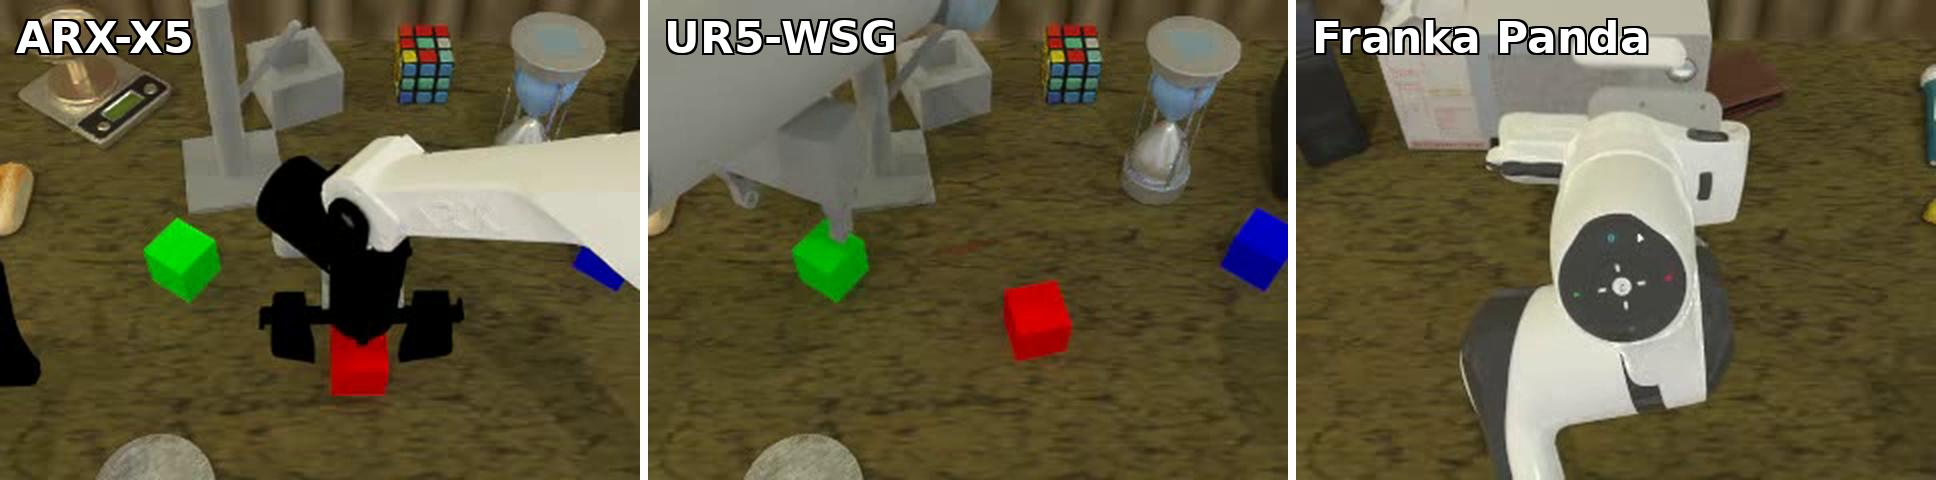
\includegraphics[width=0.8\columnwidth]{figures/fig_cross_embodiment.pdf}
% \caption{\textbf{Zero-shot cross-embodiment evaluation.} 
% % The same policy (trained on Aloha-Agilex) deployed on three unseen embodiments under randomized conditions. 
% Left: ARX. Middle: UR5. Right: Franka.
% }
% \label{fig:cross_embodiment}
% \end{figure}

% \begin{table}[!t]
% \centering
% \caption{Zero-shot cross-embodiment transfer on RoboTwin (Randomized setting). 
% % Models are trained exclusively on Aloha-Agilex demonstrations and evaluated on unseen embodiments without any target-embodiment data.
% }
% \label{tab:cross_embodiment}
% \small
% \tabcolsep 5pt
% \begin{tabular}{lcccc}
% \toprule
% & \textbf{Arx} & \textbf{UR5} & \textbf{Franka} & \textbf{Total} \\
% \midrule
% $\pi_{0.5}$ (joint)~\citep{pi05} & 24.6 & 2.2  & 0.9 & 9.2 \\
% $\pi_{0.5}$ (eef)~\citep{pi05} & 11.5 & 10.0 & 1.1 & 7.5 \\
% \midrule
% \ours (joint) & 36.4 & 3.3 & 1.4 & 13.7 \\
% \ours (eef) & 43.8 & 20.7 & 4.0 & 22.8 \\
% \bottomrule
% \end{tabular}
% \end{table}

% \subsubsection{Zero-Shot Cross-Embodiment Generalization}
% %\orange{(wangye)}
% Camera-frame relative EEF actions express deltas in the camera coordinate frame rather than a robot-specific joint space, enabling a single policy to potentially control morphologically distinct robots without re-training. 
% We test this on RoboTwin under the Randomized setting, replacing the default Aloha-Agilex with ARX-X5, UR5-WSG, and Franka Panda. 
% To isolate the effect of kinematic differences, we align the following across embodiments: (i) initial EEF poses are matched via IK; (ii) head camera and two wrist camera extrinsics are kept identical; (iii) task scenes, object layouts, and perturbation seeds are shared. 
% What remains \emph{un}aligned---and constitutes the generalization challenge---is the underlying kinematics: DOF count (6 vs.\ 7), joint arrangement, link lengths, workspace geometry, and base placement (inter-arm distance varies from 0.59--0.65\,m to accommodate different reaches). 
% The model is finetuned exclusively on RoboTwin's native clean demonstrations with the default Aloha-Agilex embodiment; no target-embodiment data is used.

% Table~\ref{tab:cross_embodiment} reports zero-shot transfer for both joint-space and camera-frame relative EEF representations. 
% Joint-space control transfers poorly: joint configurations are robot-specific, so actions meaningful for one morphology produce near-random behavior on another---UR5 and Franka stay below 3.3\% for both methods. Switching to camera-frame EEF dramatically improves transfer: \ours reaches 43.8\% on ARX, 20.7\% on UR5 ($6.3\times$ the joint result), and 4.0\% on Franka, for a cross-embodiment average of 22.8\%. 
% This confirms that the camera-frame representation successfully abstracts away morphological differences, allowing the policy to reason in shared Cartesian space. 
% Our model consistently outperforms $\pi_{0.5}$ in both action spaces, with the largest gap on UR5 (20.7 vs.\ 10.0). The performance gradient (ARX $>$ UR5 $>$ Franka) correlates with kinematic similarity to the training embodiment: ARX-X5 shares the 6-DOF form factor and similar reach as Aloha-Agilex, UR5 differs in joint arrangement but has comparable workspace, while Franka's 7-DOF kinematics and larger reach present the greatest mismatch.


\subsection{Real-World Evaluation}


\subsubsection{Evaluation on ALOHA Platforms}

\begin{figure}[!t]
\centering
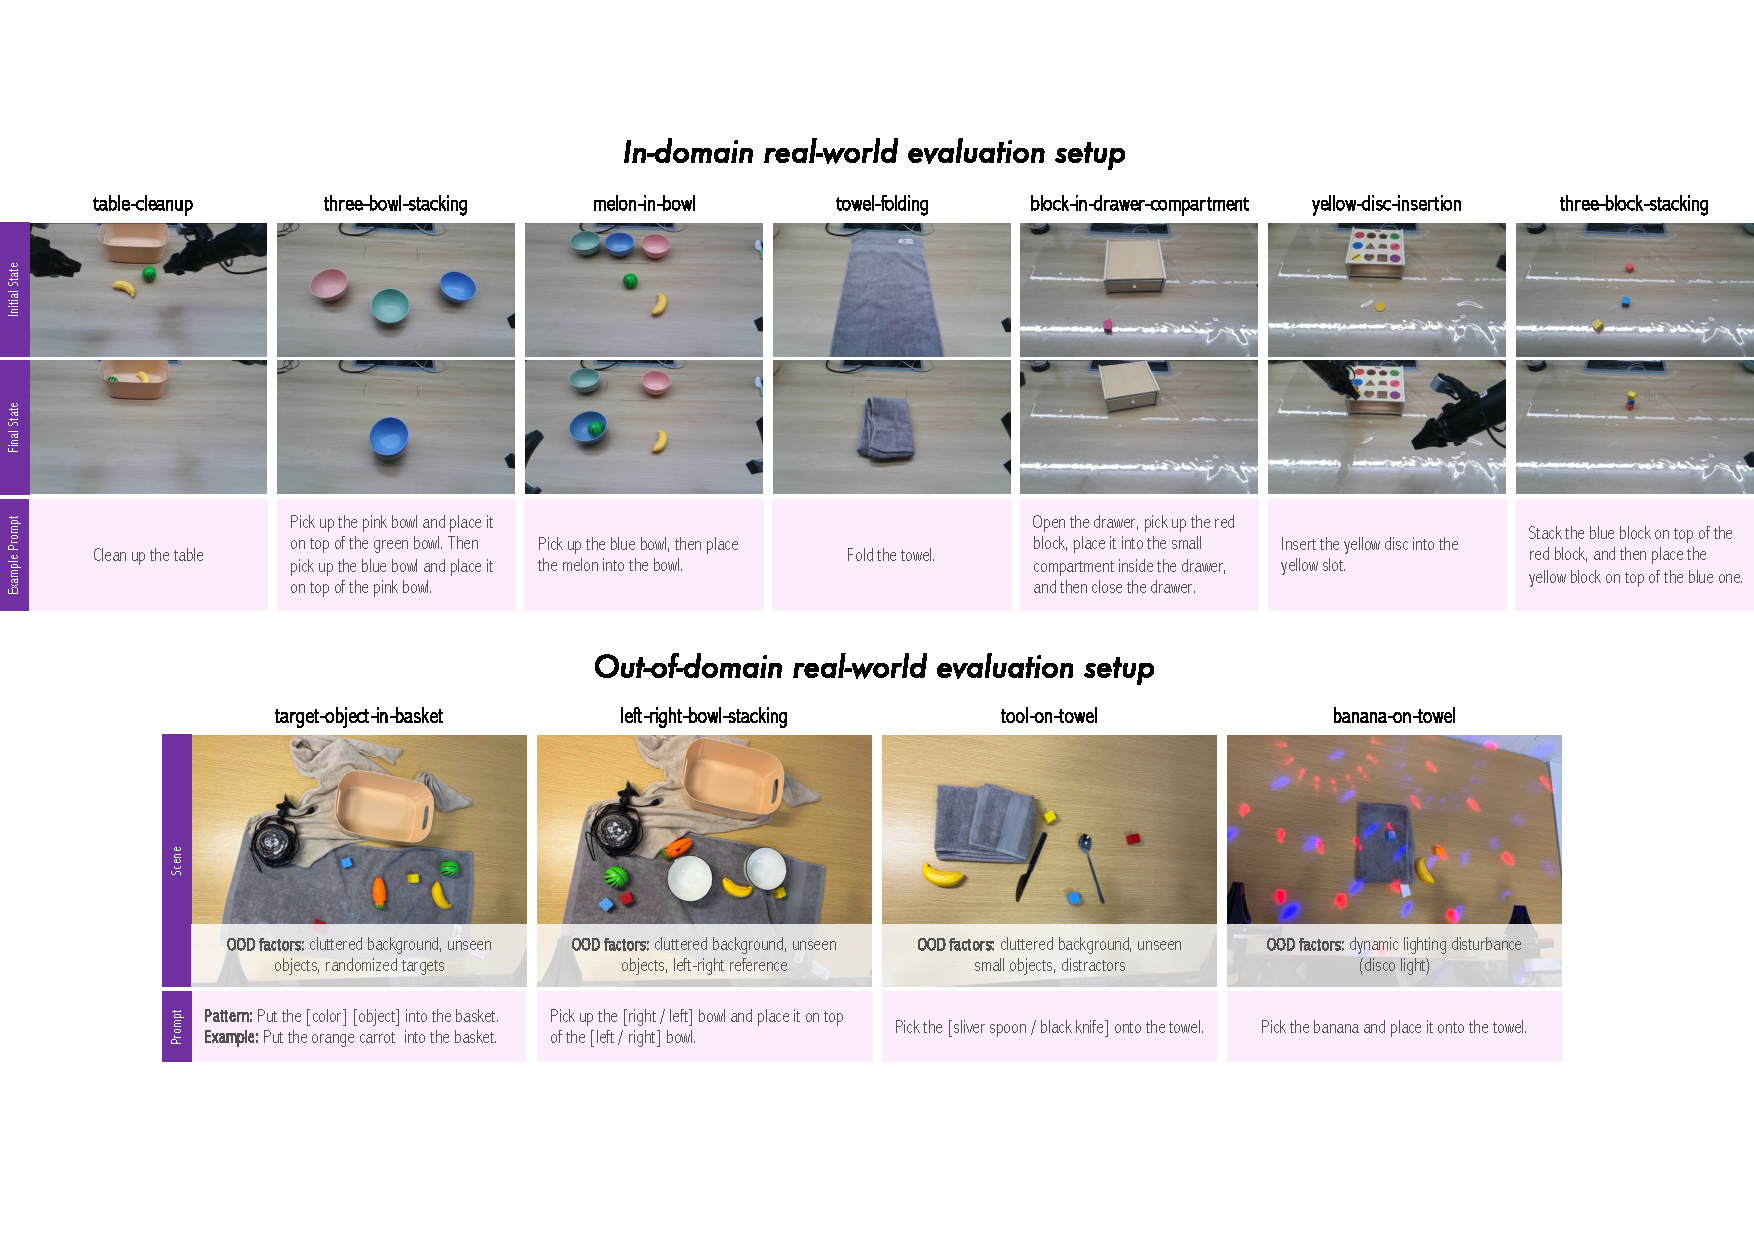
\includegraphics[width=\columnwidth]{figures/real-world-cobotmagic-setup.pdf}
\caption{\textbf{In-domain and out-of-domain tasks of real-world CobotMagic ALOHA platform.}}
\label{fig:real-world-cobotmagic-setup}
\end{figure}

\textbf{In-Domain (ID) and Out-of-Domain (OOD) Evaluation on CobotMagic ALOHA.}
We fine-tune \ours on 22.9 hours of teleoperated demonstrations collected on the CobotMagic ALOHA platform, covering multiple bimanual manipulation tasks. We then evaluate the fine-tuned policy on real-world ID and OOD benchmarks (Figure~\ref{fig:real-world-cobotmagic-setup}) constructed on the same platform.

The ID benchmark includes seven tasks: \textit{table-cleanup} (clearing objects from the table), \textit{three-bowl-stacking} (stacking three bowls in the specified order), \textit{melon-in-bowl} (placing a small spherical melon toy into a bowl), \textit{towel-folding} (folding a towel), \textit{place-block-into-drawer} (opening a drawer, placing a block inside, and closing the drawer), \textit{yellow-disc-insertion} (picking up a disc, performing a bimanual handover, and inserting it into a matching slot), and \textit{three-block-stacking} (stacking three blocks in sequence). These tasks span a wide range of manipulation difficulty.

At the easier end, \textit{table-cleanup}, \textit{three-bowl-stacking}, and \textit{melon-in-bowl} primarily test basic language grounding and sequential pick-and-place execution. \textit{Towel-folding} is more challenging due to the deformable nature of the object. The remaining tasks are substantially harder: \textit{place-block-into-drawer} is particularly challenging because it requires the robot to accurately grasp the small drawer handle and perform precise pulling and pushing motions to open and close the drawer, \textit{yellow-disc-insertion} requires fine-grained pose alignment for contact-rich insertion, and \textit{three-block-stacking} demands reliable relational reasoning and robust multi-step execution, while also testing the model's ability to recover from intermediate failures, since blocks may slip or collapse during the stacking process.

As shown in Table~\ref{tab:cobotmagic_id}, \ours achieves an average success rate of 88.6\%, significantly outperforming $\pi_{0.5}$ (42.9\%) and StarVLA (20.0\%). It succeeds in all 5 trials on five tasks and remains strong on \textit{towel-folding} (4/5). The only task with noticeable room for improvement is \textit{yellow-disc-insertion} (2/5), highlighting the difficulty of precise insertion on real hardware. In comparison, $\pi_{0.5}$ performs reasonably well on relatively simple tasks such as \textit{table-cleanup}, \textit{three-bowl-stacking}, and \textit{towel-folding}, but its performance degrades sharply on more challenging tasks that require long-horizon planning, precise contact-rich manipulation, or recovery from intermediate failures. StarVLA performs poorly across almost all tasks, with limited success even on the easier ones. These results indicate that \ours not only handles basic real-world manipulation reliably, but also scales much better to more challenging task settings.

We further evaluate real-world generalization in an out-of-domain (OOD) setting on CobotMagic ALOHA. Compared with the ID benchmark, these tasks introduce distribution shifts in visual scenes, object instances, and task instructions, and are designed to test whether the model can robustly generalize beyond the seen distribution.

\begin{table}[!t]
\centering
\caption{\textbf{In-domain real-world evaluation on the CobotMagic ALOHA platform.} We report task success over 5 trials for each task.}
\label{tab:cobotmagic_id}
\small
\setlength{\tabcolsep}{4pt}
\begin{tabular}{lccc}
\toprule
\textbf{Task} & \textbf{$\pi_{0.5}$} & \textbf{StarVLA} & \textbf{\ours} \\
\midrule
table-cleanup & 4/5 & 0/5 & 5/5 \\
three-bowl-stacking & 5/5 & 4/5 & 5/5 \\
melon-in-bowl & 2/5 & 0/5 & 5/5 \\
towel-folding & 4/5 & 3/5 & 4/5 \\
block-in-drawer-compartment & 0/5 & 0/5 & 5/5 \\
yellow-disc-insertion & 0/5 & 0/5 & 2/5 \\
three-block-stacking & 0/5 & 0/5 & 5/5 \\
\midrule
\textbf{Average success rate} & \textbf{42.9\%} & \textbf{20.0\%} & \textbf{88.6\%} \\
\bottomrule
\end{tabular}
\end{table}

\begin{table}[!t]
\centering
\caption{\textbf{Out-of-domain real-world evaluation on the CobotMagic ALOHA platform.} We report task success over 10 trials for each task.}
\label{tab:cobotmagic_ood}
\small
\setlength{\tabcolsep}{4pt}
\begin{tabular}{l p{4.3cm} ccc}
\toprule
\textbf{Task} & \textbf{OOD factors} & \textbf{$\pi_{0.5}$} & \textbf{StarVLA} & \textbf{\ours} \\
\midrule
target-object-in-basket & cluttered background, unseen objects, randomized targets & 8/10 & 0/10 & 10/10 \\
left-right-bowl-stacking & cluttered background, unseen objects, left-right reference & 1/10 & 0/10 & 10/10 \\
tool-on-towel & cluttered background, unseen small objects, distractors & 0/10 & 0/10 & 6/10 \\
banana-on-towel & dynamic lighting disturbance (disco light) & 6/10 & 0/10 & 9/10 \\
\midrule
\textbf{Average success rate} & -- & \textbf{37.5\%} & \textbf{0.0\%} & \textbf{87.5\%} \\
\bottomrule
\end{tabular}
\end{table}


The OOD benchmark contains four tasks: \textit{target-object-in-basket} (placing the instructed objects into a basket), \textit{left-right-bowl-stacking} (stacking one bowl onto another based on left-right references), \textit{tool-on-towel} (placing a specified tool onto a towel), and \textit{banana-on-towel} (placing a banana onto a towel). Each task targets a different aspect of generalization. \textit{Target-object-in-basket} introduces cluttered backgrounds, varied objects, and randomized target objects, testing whether the model can correctly identify and manipulate the instructed object under visual variation. \textit{Left-right-bowl-stacking} combines cluttered scenes and left-right relational references, requiring robust spatial language understanding. \textit{Tool-on-towel} further increases difficulty by introducing unseen and physically small objects (i.e., knife and spoon) together with distractors, making both target identification and stable grasping more difficult. Finally, \textit{banana-on-towel} evaluates robustness to severe illumination changes induced by a disco light in the real-world environment.

As shown in Table~\ref{tab:cobotmagic_ood}, \ours generalizes substantially better than the baselines in the OOD setting, achieving an average success rate of 87.5\%, compared with 37.5\% for $\pi_{0.5}$ and 0.0\% for StarVLA. In particular, \ours attains perfect success on \textit{target-object-in-basket} and \textit{left-right-bowl-stacking}, demonstrating strong robustness to cluttered scenes, attribute-based grounding, and left-right spatial references. It also remains effective on the more difficult \textit{tool-on-towel} task (6/10), where the robot must identify novel target objects under object distractors, and on \textit{banana-on-towel} (9/10) under lighting variation.

In contrast, $\pi_{0.5}$ retains some robustness on relatively simpler OOD variations, achieving 8/10 on \textit{target-object-in-basket} and 6/10 on \textit{banana-on-towel}. However, its performance collapses on tasks requiring stronger compositional and relational generalization, obtaining only 1/10 on \textit{left-right-bowl-stacking} and 0/10 on \textit{tool-on-towel}. StarVLA fails on all four OOD tasks. These results suggest that \ours preserves much stronger visual-linguistic representation and is considerably more robust to scene clutter, novel objects, spatial references, and lighting changes in real-world settings.


% CobotMagic: \orange{(linpei, wangye, haoyang)}
% - 20+ tasks, 6k+ trajs
% - Construct OOD scene and task eval <TODO>
% - Long-horizon instruction following (agentic?) <TODO>



% Arx: <TODO> \orange{(wangye, linpei, haoyang)}
% Today

% \textbf{Stand Bottle}
% \begin{table}[!t]
% \centering
% \caption{Real World Arx}
% \label{tab:real_arx}
% \small
% \tabcolsep 3pt
% \begin{tabular}{lccccccc}
% \toprule
% & \textbf{Put Fruits} & \textbf{Put Blocks} & \textbf{Fold Towel} & \textbf{Sweep Trash} & \textbf{Insert Screw} & \textbf{Unscrew Cap} \\
% \midrule
% StarVLA~\citep{community2026starvla} & 10.0 & 5.0 & 0.0 & 0.0 & 0.0 & 13.3 \\
% $\pi_{0.5}$~\citep{pi05} & 55.0 & 17.5 & 20.0 & 8.8 & 6.3 & 33.3 \\
% \midrule
% \ours & 56.4 & 37.5 & 25.0 & 5.0 & 6.3 & 39.9 \\
% % \ours (eef) & \blue{69.9} & -- & -- & -- & -- & \blue{59.5} \\
% \bottomrule
% \end{tabular}
% \end{table}

\begin{figure}[!t]
\centering
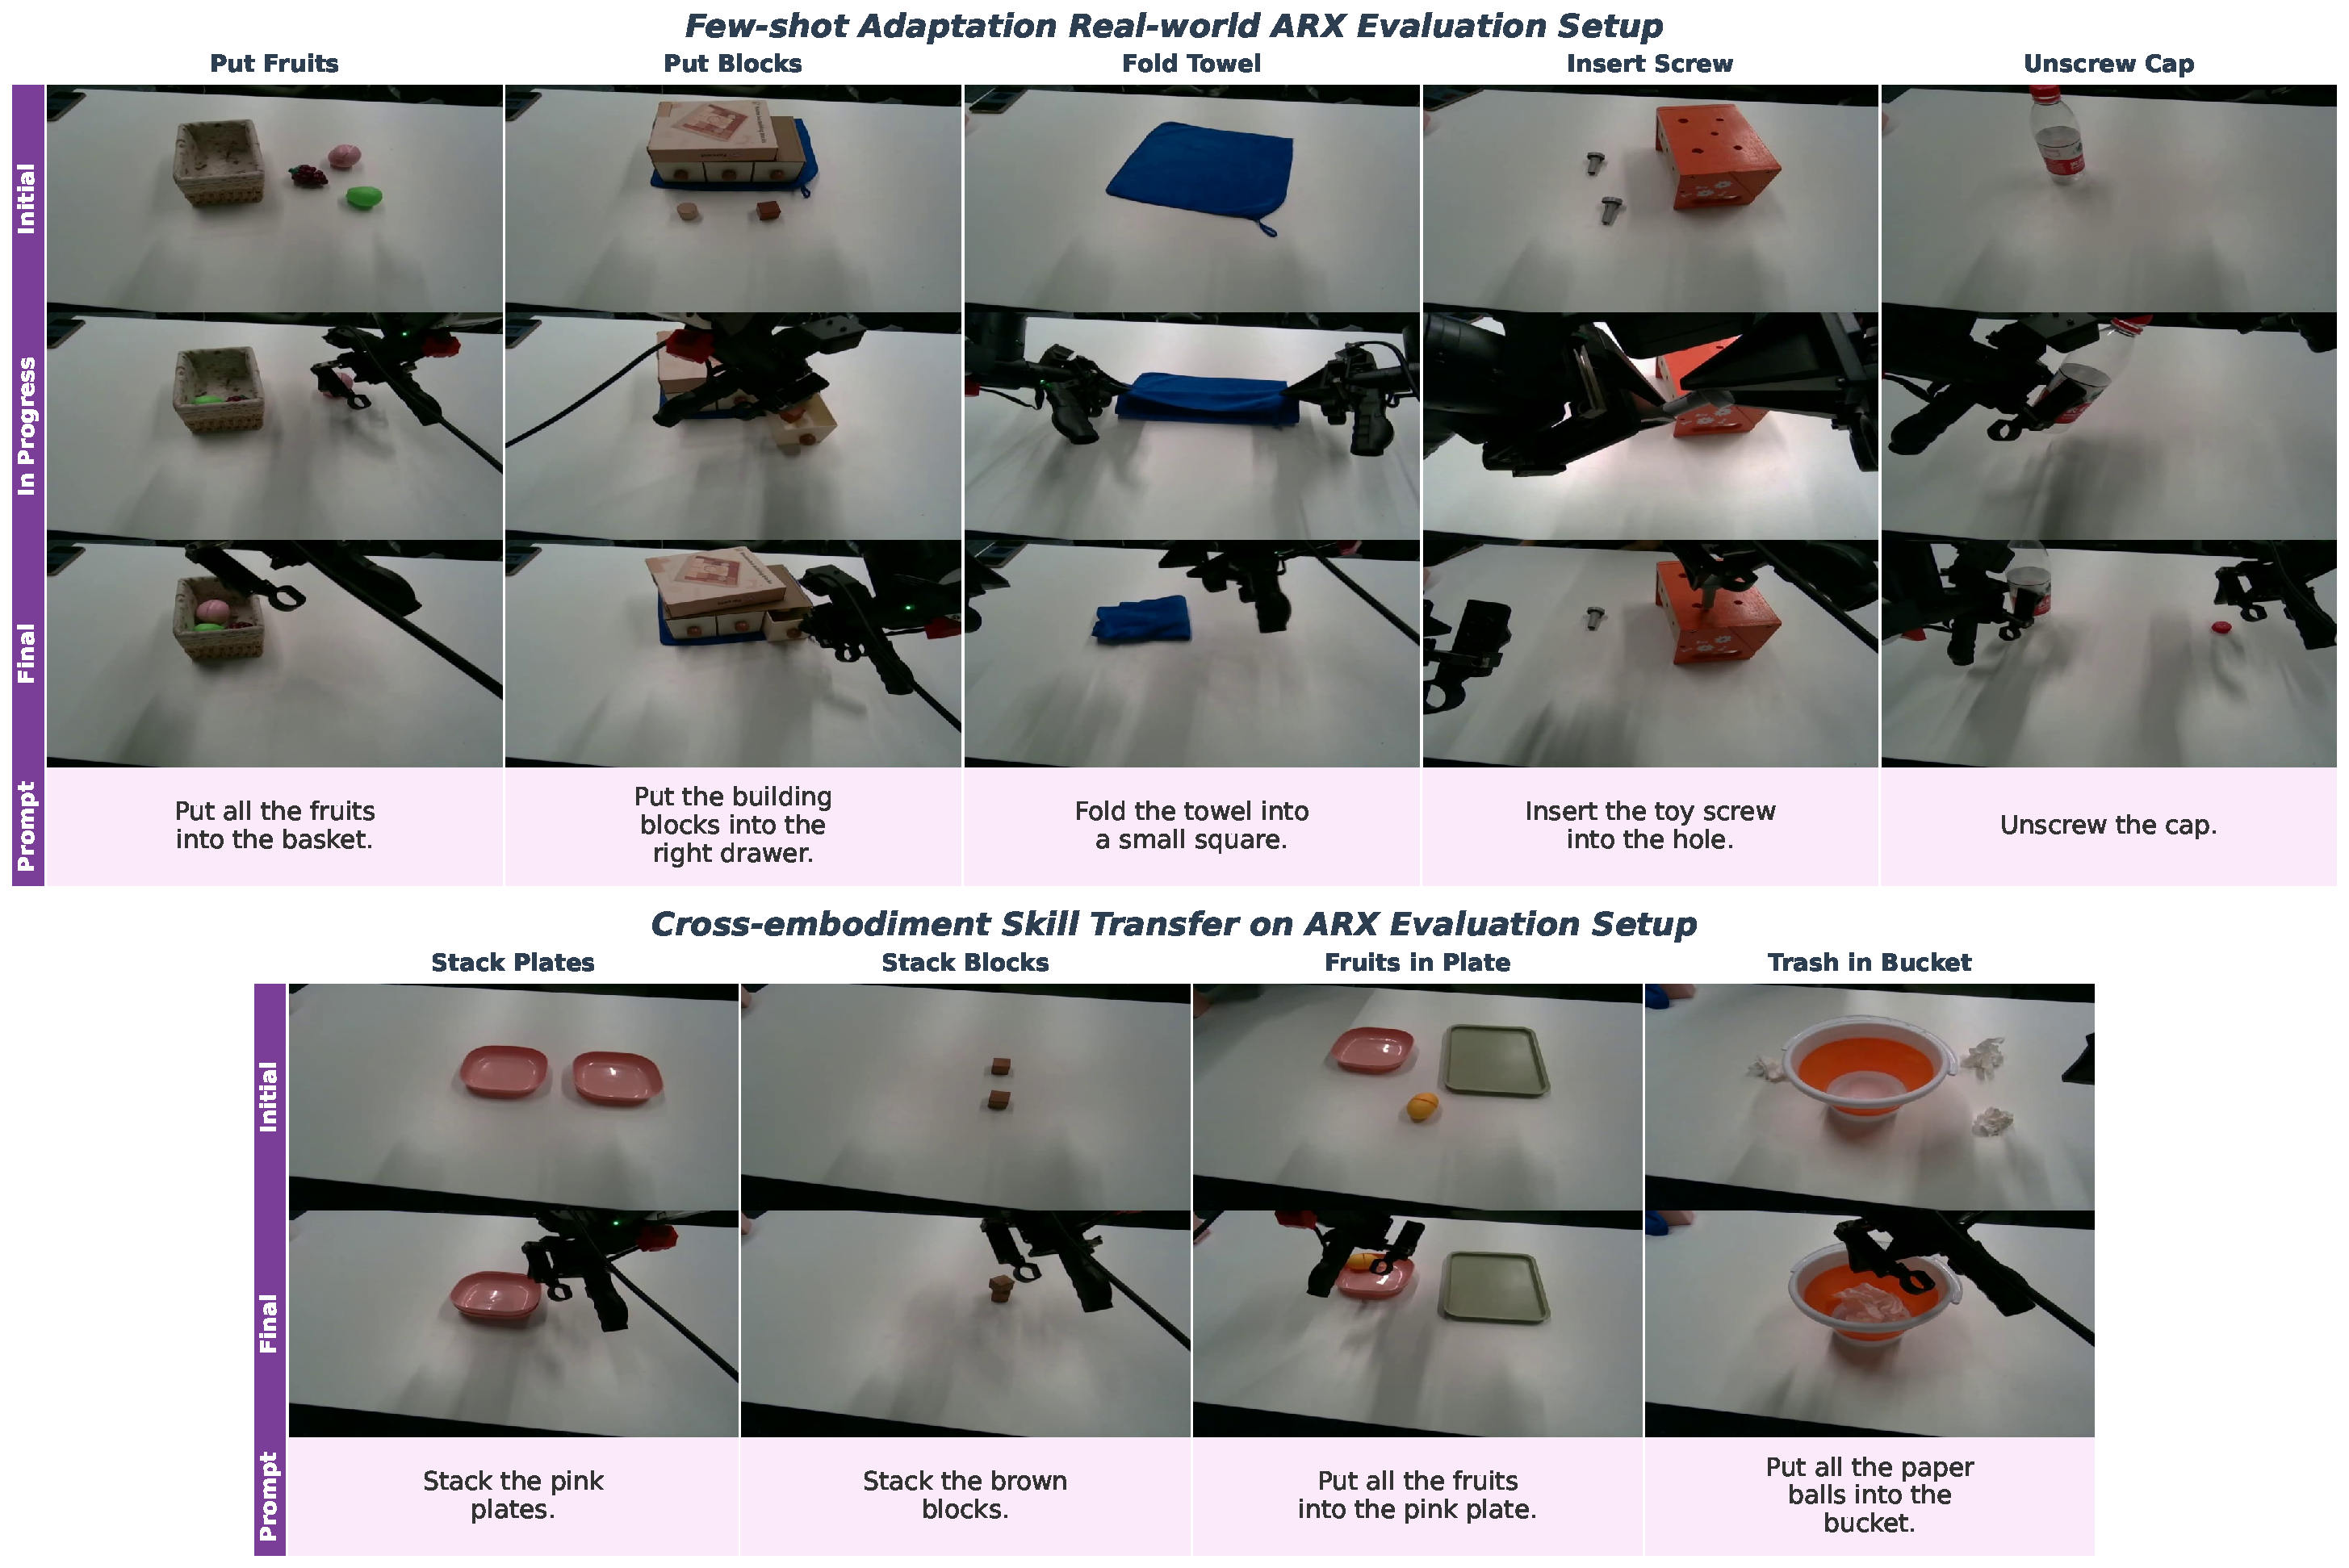
\includegraphics[width=\columnwidth]{figures/arx_evaluation_setup.pdf}
\caption{\textbf{Real-world evaluation setup on the ARX ALOHA platform.}}
\label{fig:real-world-arx-setup}
\end{figure}

\begin{table}[!t]
\centering
\caption{\textbf{Few-shot adaptation on ARX ALOHA.} Sub-step success over 10 trials. All methods are jointly fine-tuned on 130 teleoperated demonstrations (50 for Unscrew Cap, 20 for each other task).}
\label{tab:real_arx}
\small
\setlength{\tabcolsep}{4pt}
\begin{tabular}{ll ccc}
\toprule
\textbf{Task} & \textbf{Sub-step} & \textbf{StarVLA} & \textbf{$\pi_{0.5}$} & \textbf{\ours} \\
\midrule
\multirow{4}{*}{Put Fruits} 
& Place fruit 1 & 3/10 & 9/10 & 9/10 \\
& Place fruit 2 & 1/10 & 5/10 & 5/10 \\
& Place fruit 3 & 0/10 & 2/10 & \textbf{3/10} \\
& \cellcolor{gray!10}\textit{Avg. success} & \cellcolor{gray!10}13.3\% & \cellcolor{gray!10}53.3\% & \cellcolor{gray!10}\textbf{56.7\%} \\
\midrule
\multirow{5}{*}{Put Blocks}
& Open drawer & 1/10 & 4/10 & \textbf{5/10} \\
& Place block 1 & 1/10 & 2/10 & \textbf{4/10} \\
& Place block 2 & 0/10 & 2/10 & \textbf{3/10} \\
& Close drawer & 0/10 & 2/10 & \textbf{3/10} \\
& \cellcolor{gray!10}\textit{Avg. success} & \cellcolor{gray!10}5.0\% & \cellcolor{gray!10}25.0\% & \cellcolor{gray!10}\textbf{37.5\%} \\
\midrule
\multirow{3}{*}{Fold Towel}
& First fold & 0/10 & 3/10 & 3/10 \\
& Second fold & 0/10 & 1/10 & \textbf{3/10} \\
& \cellcolor{gray!10}\textit{Avg. success} & \cellcolor{gray!10}0.0\% & \cellcolor{gray!10}20.0\% & \cellcolor{gray!10}\textbf{30.0\%} \\
\midrule
\multirow{3}{*}{Insert Screw}
& Handover screw & 0/10 & 2/10 & 2/10 \\
& Insert screw & 0/10 & 0/10 & 0/10 \\
& \cellcolor{gray!10}\textit{Avg. success} & \cellcolor{gray!10}0.0\% & \cellcolor{gray!10}10.0\% & \cellcolor{gray!10}10.0\% \\
\midrule
\multirow{4}{*}{Unscrew Cap}
& Grasp bottle & 4/10 & 9/10 & 9/10 \\
& Unscrew cap & 0/10 & 2/10 & \textbf{4/10} \\
& Place down & 0/10 & 1/10 & \textbf{3/10} \\
& \cellcolor{gray!10}\textit{Avg. success} & \cellcolor{gray!10}13.3\% & \cellcolor{gray!10}40.0\% & \cellcolor{gray!10}\textbf{53.3\%} \\
\bottomrule
\end{tabular}
\end{table}

\textbf{Few-shot Adaptation on ARX ALOHA.}
We compare \ours against two baselines on five real-world manipulation tasks (Figure~\ref{fig:real-world-arx-setup}, top; Table~\ref{tab:real_arx}): $\pi_{0.5}$~\citep{pi05}, a pretrained open-source VLA, and StarVLA~\citep{community2026starvla} trained from scratch without pretraining. 
All methods use joint positions and EEF pose as state and predict actions in EEF space, jointly fine-tuned on the same 130 teleoperated demonstrations (50 for Unscrew Cap, 20 for each other task). 
The five tasks span multi-object pick-and-place (Put Fruits), long-horizon sequential manipulation (Put Blocks), deformable object handling (Fold Towel), bimanual precision assembly (Insert Screw), and fine-grained rotational control (Unscrew Cap).

\ours outperforms both baselines on four of five tasks. The largest gain appears on Put Blocks (15/40 vs.\ 10/40 for $\pi_{0.5}$), where \ours maintains higher sub-step success through all four stages---open drawer, place two blocks, and close drawer---indicating more robust long-horizon execution. 
On Unscrew Cap, \ours doubles the cap-removal rate over $\pi_{0.5}$ (4/10 vs.\ 2/10) and triples the full-task completion (3/10 vs.\ 1/10), showing stronger fine-grained rotational control. 
Fold Towel improves notably on the second fold (3/10 vs.\ 1/10). 
Insert Screw remains challenging for all methods, with no model completing a full insertion (0/10), though both $\pi_{0.5}$ and \ours succeed at the handover sub-step (2/10). 
StarVLA, without pretraining, achieves near-zero across tasks, confirming the importance of large-scale pretraining for real-world manipulation.

\begin{table}[!t]
\centering
\caption{\textbf{Cross-embodiment skill transfer on ARX.}}
\label{tab:cross_embodiment_transfer}
\small
\tabcolsep 3pt
\begin{tabular}{lccccc}
\toprule
& \textbf{Stack Plates} & \textbf{Stack Blocks} & \textbf{Fruits in Plate} & \textbf{Trash in Bucket} & \textbf{Avg.} \\
\midrule
\ours w/o UnifiedSpace & 0/10 & 0/10 & 3/10 & 0/10 & 7.5\% \\
\ours w/o UnifiedEEF & 0/10 & 0/10 & 5/10 & 0/10 & 12.5\% \\
\midrule
\ours & \textbf{3/10} & \textbf{5/10} & \textbf{7/10} & \textbf{7/10} & \textbf{55.0\%} \\
\bottomrule
\end{tabular}
\end{table}

\textbf{Cross-embodiment transfer.}
% SFT on 6k cobot + 130 ARX  already: execute ARX tasks on the cobot + cobot tasks on ARX. (eef control)
% - Cross-embodiment generalization (task transfer to cobotmagic?)
We also investigate cross-embodiment skill transfer (Figure~\ref{fig:real-world-arx-setup}, bottom; Table~\ref{tab:cross_embodiment_transfer}). 
A single policy is jointly fine-tuned on 6K CobotMagic and 130 ARX demonstrations, using the same state-action parameterization as above, then evaluated on four novel tasks on the ARX platform: stacking two plates, stacking blocks, placing fruits into a designated pink plate with distractor plates, and collecting paper balls into a bucket. 
ARX has \emph{zero demonstrations} for any of these tasks---the relevant manipulation skills (stacking, precise placement, object collection) must generalize from related but not identical CobotMagic behaviors across a kinematically different embodiment. 
We ablate two key components: \ours w/o UnifiedSpace removes the unified action-space mapping and instead naively concatenates and zero-pads each robot's action dimensions without semantic alignment; \ours w/o UnifiedEEF removes the unified EEF representation while retaining a basic slot layout with rotation unification and gripper normalization. 
Both variants fail almost entirely (7.5\% and 12.5\%), showing that neither surface-level dimension alignment nor partial unification can bridge the combined embodiment and task gap. 
\ours achieves 55.0\%---over 4$\times$ the best variant---succeeding on all four tasks including Stack Blocks (5/10) and Trash in Bucket (7/10). 
The full unified action space and EEF representation enable \ours to learn a stronger manipulation representation through large-scale diverse pretraining, enabling skill-level transfer: a policy can leverage skills learned from one embodiment to execute novel tasks on another embodiment with minimal training data and no task-specific demonstrations.
% a policy can leverage related experience from one embodiment to solve novel tasks on a different robot it has barely trained on.
% * The specific tasks are only determined after the trial begins.* 

% \textbf{Few shot OOD?}
% SFT on 100 ARX: different light/object/instruction)


% \subsection{Qualitative Analysis}
% - human2robot vis

\subsubsection{Table30-v1 Challenge}


\begin{table*}[!t]
\centering
\caption{\textbf{Per-task results on the RoboChallenge Table30 v1 Generalist Track.} Each cell reports success rate (\%) / process score. Best results per task are in \textbf{bold}.}
\label{tab:table30_results}
\resizebox{\textwidth}{!}{
\begin{tabular}{llccccc}
\toprule
Robot & Task & \ours & DM0\_generalist & pi05\_generalist & GR00T-MULTI & pi0\_generalist \\
\midrule
\multicolumn{2}{l}{\textbf{Average (all)}} & \textbf{45 / 59.83} & 37 / 48.43 & 17.67 / 31.27 & 15.33 / 32.29 & 9 / 20.22 \\
\midrule
\multirow{12}{*}{ARX5}
& arrange flowers & \textbf{30 / 64} & 20 / 49 & 0 / 30.5 & 20 / 57 & 0 / 13.5 \\
& arrange paper cups & \textbf{70 / 83} & 10 / 54 & 0 / 31 & 0 / 19 & 0 / 15 \\
& fold dishcloth & \textbf{30 / 48} & 10 / 10.5 & 0 / 0 & 0 / 17 & 0 / 0 \\
& open the drawer & 0 / 47 & \textbf{90 / 95} & 50 / 80 & 0 / 50 & 0 / 20 \\
& place shoes on rack & 70 / 85 & \textbf{100 / 98.5} & 0 / 20 & 40 / 54.5 & 0 / 16.5 \\
& put cup on coaster & 100 / 99 & \textbf{100 / 100} & 70 / 63 & 80 / 92 & 0 / 0 \\
& search green boxes & 90 / 92 & \textbf{100 / 95.5} & 0 / 3 & 30 / 37.5 & 0 / 0 \\
& sort electronic products & \textbf{50 / 60.4} & 0 / 18.4 & 0 / 22.5 & 10 / 34.8 & 0 / 22.5 \\
& turn on light switch & 70 / 69.5 & \textbf{70 / 70.5} & 10 / 25 & 0 / 5 & 20 / 29 \\
& water potted plant & 0 / 9 & 0 / \textbf{33.5} & 0 / 0 & 0 / 6 & 0 / 0 \\
& wipe the table & 0 / \textbf{72.5} & 0 / 47.5 & 10 / 28 & 0 / 66 & 0 / 29 \\
\addlinespace[2pt]\cmidrule{2-7}\addlinespace[2pt]
& \textit{Avg (ARX5)} & \textbf{\textit{46.4 / 66.3}} & \textit{45.5 / 61.1} & \textit{12.7 / 27.5} & \textit{16.4 / 39.9} & \textit{1.8 / 13.2} \\
\midrule
\multirow{12}{*}{ALOHA}
& clean dining table & 20 / 57.5 & 0 / 12 & \textbf{30 / 62} & 10 / 11.5 & 0 / 25.5 \\
& make vegetarian sandwich & \textbf{10 / 46.5} & 0 / 15 & 0 / 0 & 0 / 7 & 0 / 0 \\
& plug in network cable & \textbf{30 / 51} & 10 / 26 & 0 / 0 & 0 / 3 & 0 / 0 \\
& pour fries into plate & \textbf{30 / 56} & 0 / 6 & 0 / 0 & 0 / 36 & 0 / 0 \\
& put opener in drawer & 0 / 0 & 10 / 10 & \textbf{20 / 38} & 0 / 0 & 0 / 0 \\
& put pen into pencil case & \textbf{90 / 95} & 20 / 40 & 50 / 63.5 & 20 / 58 & 0 / 14.5 \\
& scan QR code & 10 / 13 & 0 / 0 & 0 / 7 & \textbf{30 / 26.5} & 0 / 3 \\
& stack bowls & \textbf{100 / 98.5} & 70 / 71 & 80 / 83 & 40 / 55.5 & 40 / 53.5 \\
& stick tape to box & 0 / \textbf{22.5} & 0 / 14 & 0 / 16 & 0 / 2 & 0 / 0 \\
& sweep the rubbish & \textbf{70 / 84.5} & 30 / 40 & 10 / 46 & 10 / 10 & 0 / 17 \\
& turn on faucet & \textbf{100 / 100} & 70 / 84.5 & 60 / 56 & 20 / 44 & 60 / 67.5 \\
\addlinespace[2pt]\cmidrule{2-7}\addlinespace[2pt]
& \textit{Avg (ALOHA)} & \textbf{\textit{41.8 / 56.8}} & \textit{19.1 / 29.0} & \textit{22.7 / 33.8} & \textit{11.8 / 23.0} & \textit{9.1 / 16.5} \\
\midrule
\multirow{7}{*}{UR5}
& arrange fruits in basket & \textbf{80 / 89.5} & 70 / 87 & 0 / 9 & 30 / 54.5 & 0 / 11.5 \\
& hang toothbrush cup & 60 / 80 & \textbf{90 / 95} & 50 / 71 & 70 / 85 & 20 / 62 \\
& set the plates & \textbf{100 / 87.5} & 60 / 62 & 40 / 49.5 & 0 / 24 & 50 / 69.5 \\
& shred scrap paper & 0 / 15 & \textbf{30 / 45} & 20 / 36 & 0 / 0 & 20 / 27 \\
& sort books & 0 / 9 & 0 / 8.5 & 0 / 24 & 0 / 6.5 & \textbf{10 / 26.5} \\
& stack color blocks & 70 / 84.5 & \textbf{100 / 100} & 10 / 30 & 0 / 44.5 & 30 / 39 \\
\addlinespace[2pt]\cmidrule{2-7}\addlinespace[2pt]
& \textit{Avg (UR5)} & \textit{51.7 / 60.9} & \textbf{\textit{58.3 / 66.2}} & \textit{20.0 / 36.6} & \textit{16.7 / 35.8} & \textit{21.7 / 39.2} \\
\midrule
\multirow{3}{*}{Franka}
& move objects into box & \textbf{70 / 75.5} & 50 / 64.5 & 20 / 40 & 50 / 62 & 20 / 44.5 \\
& press three buttons & 0 / 0 & 0 / 0 & 0 / \textbf{4} & 0 / 0 & 0 / 0 \\
\addlinespace[2pt]\cmidrule{2-7}\addlinespace[2pt]
& \textit{Avg (Franka)} & \textbf{\textit{35.0 / 37.8}} & \textit{25.0 / 32.2} & \textit{10.0 / 22.0} & \textit{25.0 / 31.0} & \textit{10.0 / 22.2} \\
\bottomrule
\end{tabular}
}
\end{table*}



% \orange{(haoyang)}
To evaluate the generalization capability of \ours, we submit to the RoboChallenge Table30 v1 benchmark under the generalist track. This benchmark comprises 30 manipulation tasks distributed across 4 robot embodiments, and offers two evaluation tracks: the \textit{specialist} track, where a dedicated policy is trained for each individual task (requiring 30 separate models), and the \textit{generalist} track, where a single unified policy is trained per embodiment to handle all tasks associated with that robot. The generalist setting is substantially more challenging, as it demands that the policy generalize across diverse manipulation skills within each embodiment rather than overfitting to a single task. We focus on this track as it better reflects real-world desideratum of building versatile manipulation policies.

Specifically, we post-train \ours on the demonstration data provided by Table30 v1 using joint control, and submit under the anonymous identity \texttt{Lira\_generalist}\footnote{See \texttt{Lira\_generalist} in \url{https://robochallenge.cn/home}.}. \ours achieves a success rate of 45\% and a process score of 59.83. Notably, \ours surpasses \texttt{DM0\_generalist} (37\% success rate, 48.43 process score) by 8 percentage points in success rate and 11.4 in process score, demonstrating its strong multi-task generalization ability. We highlight three key findings from detailed analysis of the benchmark results.

\paragraph{Strong bimanual coordination.}
Among the 30 benchmark tasks, 8 require tight bimanual coordination on the ALOHA platform\footnote{The 8 bimanual tasks: \textit{clean dining table}, \textit{make vegetarian sandwich}, \textit{pour fries into plate}, \textit{put opener in drawer}, \textit{put pen into pencil case}, \textit{stick tape to box}, \textit{sweep the rubbish}, \textit{turn on faucet}.}, where the two arms must jointly stabilize, transport, and manipulate objects. \ours achieves an average success rate of 40\% on these tasks, far exceeding $\pi_{0.5}$ (21.2\%), DM0 (16.2\%), GR00T-MULTI (7.5\%), and $\pi_{0}$ (7.5\%) (Figure~\ref{fig:bimanual_pickplace_bar}, left). Notably, \ours is the \emph{only} model to succeed on \textit{pour fries into plate} (30\% vs.\ 0\% for all baselines), a task demanding sequential bimanual steps---stabilizing the fries box with the left arm, opening it with the right arm, picking it up, and pouring the contents onto the plate. As illustrated in Figure~\ref{fig:case_bimanual}, \ours completes this full sequence, while DM0\_generalist fails at the initial coordination stage: the right arm never reaches a graspable position on the box, resulting in immediate task failure. We attribute this strong bimanual performance to two factors: (1)~our pre-training corpus contains a substantial proportion of bimanual demonstration robot data, enabling the model to effectively learn coordinated dual-arm control primitives; and (2)~our Human2Robot pipeline, which synthesizes bimanual robot data from egocentric human videos, further expands the effective bimanual pre-training data and exposes the model to diverse manipulation strategies beyond those captured in teleoperated demonstrations alone.

\begin{figure}[!t]
    \centering
    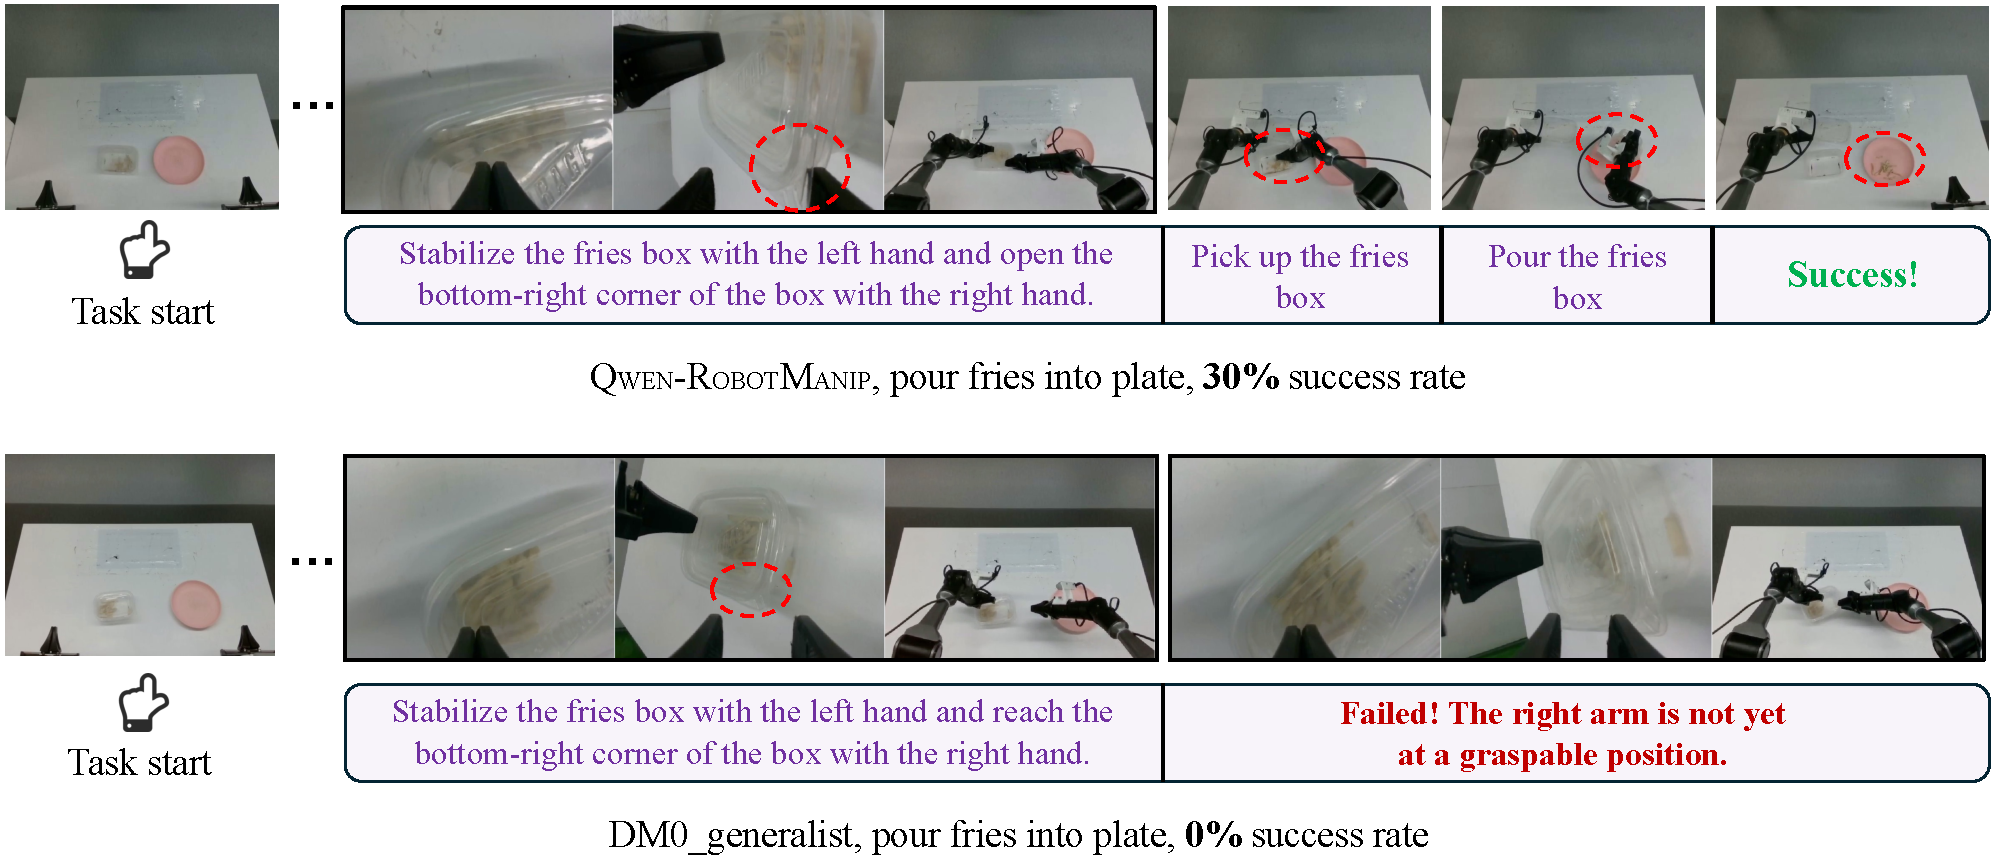
\includegraphics[width=\linewidth]{figures/case_study-bimanual.pdf}
    \caption{\textbf{Case study on \textit{pour fries into plate} (ALOHA).} \ours (top) coordinates both arms to stabilize, open, pick up, and pour the fries box, completing the task successfully. DM0\_generalist (bottom) fails at the initial stage as the right arm never reaches a graspable position.}
    \label{fig:case_bimanual}
\end{figure}

\begin{figure}[!t]
    \centering
    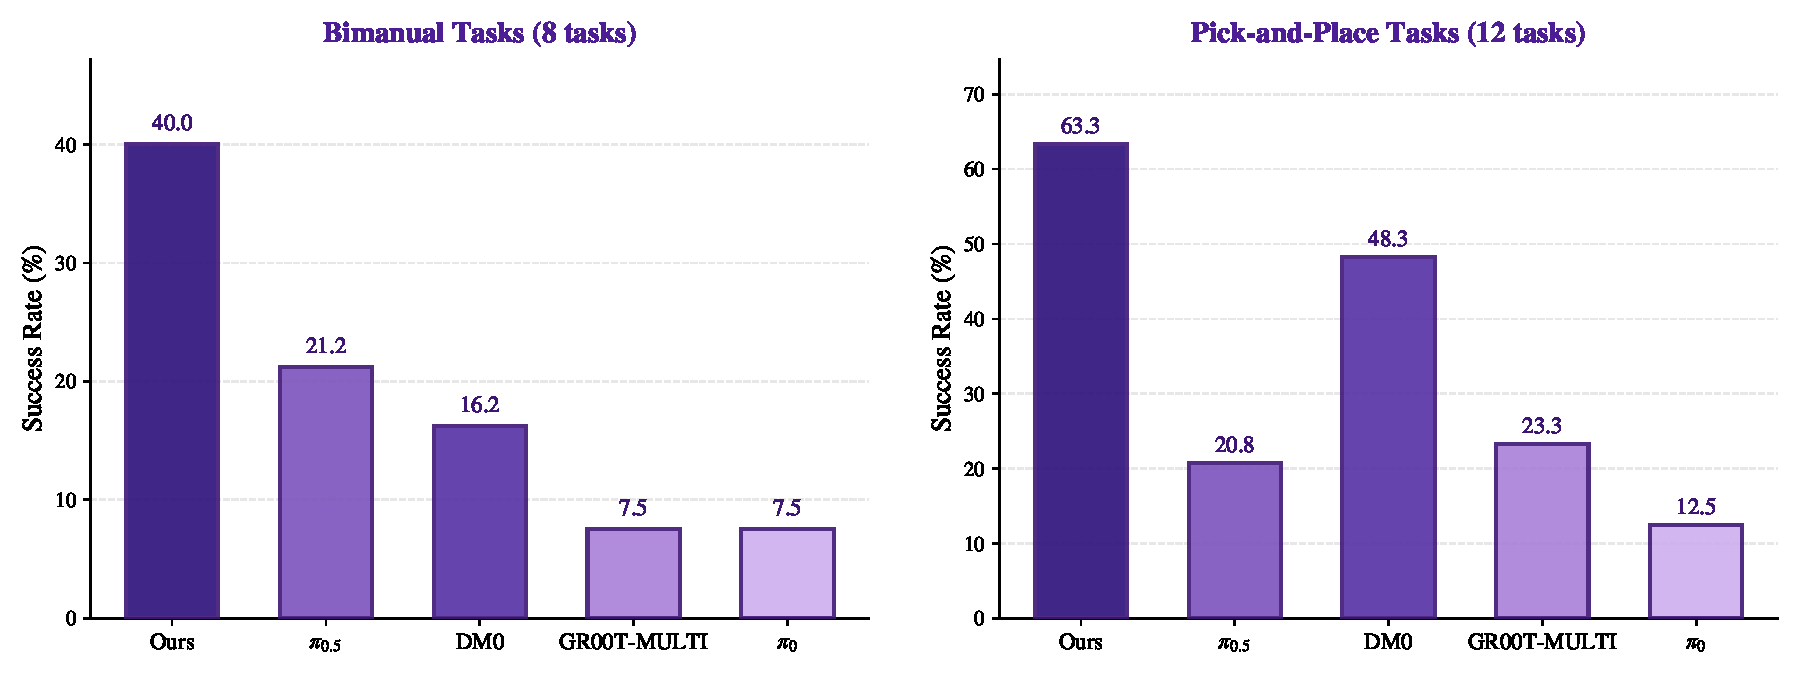
\includegraphics[width=\linewidth]{figures/bimanual_pickplace_bar.pdf}
    \caption{\textbf{Average success rate on bimanual coordination tasks (left, 8 tasks) and pick-and-place tasks (right, 12 tasks).} \ours substantially outperforms all baselines in both categories.}
    \label{fig:bimanual_pickplace_bar}
\end{figure}

\paragraph{Robust pick-and-place across embodiments.}
We identify 12 tasks across all four platforms that center on pick-and-place primitives\footnote{The 12 pick-and-place tasks are: \textit{arrange flowers}, \textit{arrange fruits in basket}, \textit{arrange paper cups}, \textit{clean dining table}, \textit{move objects into box}, \textit{set the plates}, \textit{sort books}, \textit{sort electronic products}, \textit{stack bowls}, \textit{place shoes on rack}, \textit{put cup on coaster}, and \textit{stack color blocks}.}, ranging from single-object grasping (\textit{put cup on coaster} and \textit{stack color blocks}) to multi-step sequential manipulation involving 4--5 objects (\textit{arrange paper cups} and \textit{sort electronic products}). As shown in Figure~\ref{fig:bimanual_pickplace_bar}~(right), \ours achieves 63.3\% average success rate on these tasks, surpassing the next-best baseline DM0 (48.3\%) by 15.0 percentage points.  We attribute this capability to two factors: (1)~the large-scale cross-embodiment pre-training data encodes abundant pick-and-place patterns, and (2)~the unified action space enables knowledge sharing of fundamental spatial skills across different robot morphologies. Figure~\ref{fig:case_pickplace} shows a representative comparison on \textit{arrange paper cups}, a task requiring sequential pick-and-place of multiple cups followed by stacking. \ours (70\% SR) successfully picks each cup in sequence, stacks them precisely, while $\pi_{0.5}$\_generalist (0\% SR) encounters a stuck cup during stacking and fails to recover, leading to cascading errors in subsequent steps.

\begin{figure}[!t]
    \centering
    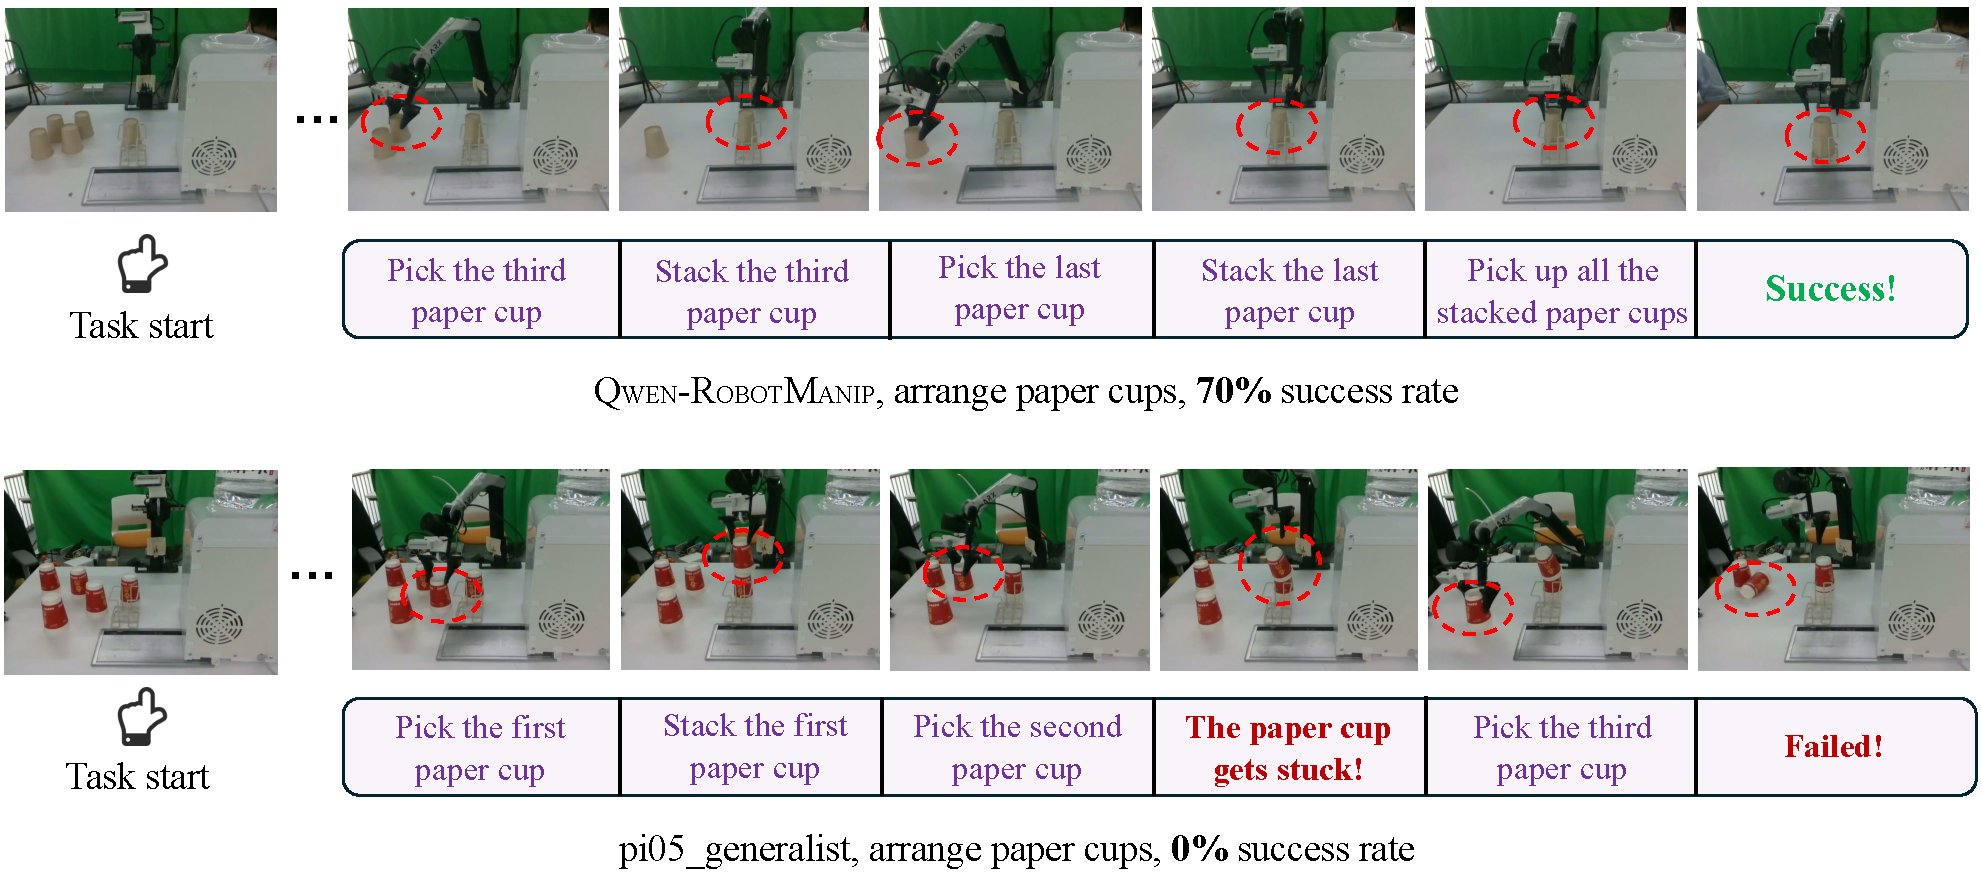
\includegraphics[width=\linewidth]{figures/case_study-repeat.pdf}
    \caption{\textbf{Case study on \textit{arrange paper cups} (ARX5).} \ours (top) sequentially picks, stacks, and collects all paper cups with precise placement. $\pi_{0.5}$\_generalist (bottom) encounters a stuck cup during stacking and fails to recover.}
    \label{fig:case_pickplace}
\end{figure}

\paragraph{Emergent retry behavior.}
A recurring pattern we observe during real-robot evaluation is that \ours exhibits spontaneous retry behavior: when an initial manipulation attempt fails (e.g., a grasp slips or a placement misses) the policy autonomously re-attempts the action rather than proceeding to the next step or stalling. While this behavior is difficult to quantify with a single metric, we observe it consistently across diverse action primitives including picking, placing, pouring, folding, wiping, and sweeping. This self-corrective capability significantly improves fault tolerance, allowing \ours to recover from intermediate failures that would otherwise cause task-level failures. Figure~\ref{fig:case_retry} provides a vivid example on \textit{sort electronic products}: \ours successfully picks up the object on its first attempt, but the object falls; it then re-attempts, and the object falls again; on the third attempt, \ours finally completes the grasp and places the object into the target bin, achieving task success (50\% SR). In contrast, DM0\_generalist (0\% SR) also attempts the pick three times but fails every attempt---the gripper never achieves a secure grasp, leading to task failure. We hypothesize that this retry behavior emerges from the diversity of the pre-training data, where demonstrations naturally contain imperfect attempts followed by corrections, enabling the model to learn recovery strategies as part of its policy.

\begin{figure}[!t]
    \centering
    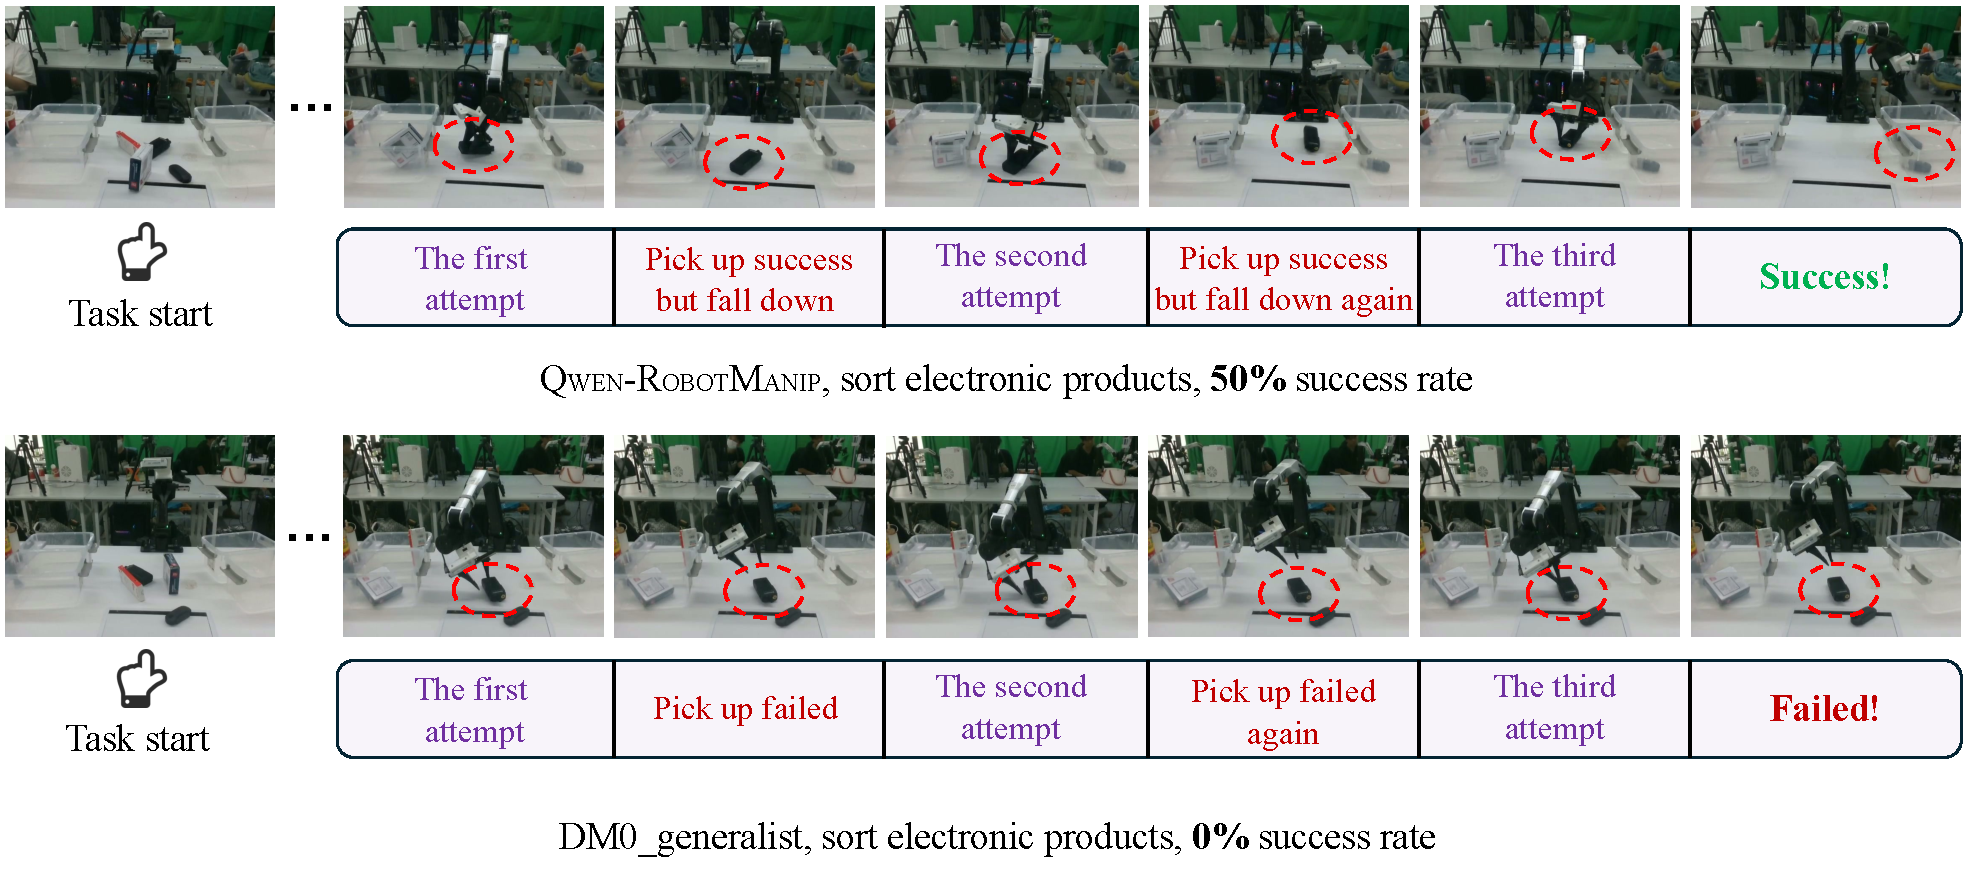
\includegraphics[width=\linewidth]{figures/case_study-retry.pdf}
    \caption{\textbf{Case study on \textit{sort electronic products} (ARX5).} \ours (top) picks up the object but it falls twice; the policy autonomously retries and succeeds on the third attempt. DM0\_generalist (bottom) also attempts three times but never achieves a secure grasp.}
    \label{fig:case_retry}
\end{figure}

% \begin{figure}[htb]
%     \centering
%     \includegraphics[width=0.5\linewidth]{figures/table30v1-generalist.jpg}
%     \caption{\textbf{RoboChallenge Table30 v1 Generalist Leaderboard.} }
%     \label{fig:table30v1}
% \end{figure}

% \textbf{Per-embodiment analysis.} As shown in Table~\ref{tab:table30_results}, \ours achieves the highest average success rate on three out of four robot platforms: ARX5 (46.4\%), ALOHA (41.8\%), and Franka (35.0\%). On UR5, \ours ranks second (51.7\%) behind DM0\_generalist (58.3\%). The strong and consistent performance across diverse robot embodiments can thus be attributed to the large-scale cross-embodiment pre-training of \ours, which provides a robust foundation that readily adapts to each platform with embodiment-specific fine-tuning.

% \begin{figure}[t]
% \centering
% \includegraphics[width=\textwidth]{figures/core_skills_filmstrip.png}
% \vspace{-15pt}
% \caption{Qualitative results on core manipulation tasks. Each row shows uniformly sampled frames from one evaluation episode.}
% \label{fig:core_skills}
% \vspace{-2pt}
% \end{figure}

\begin{figure}[!t]
\centering
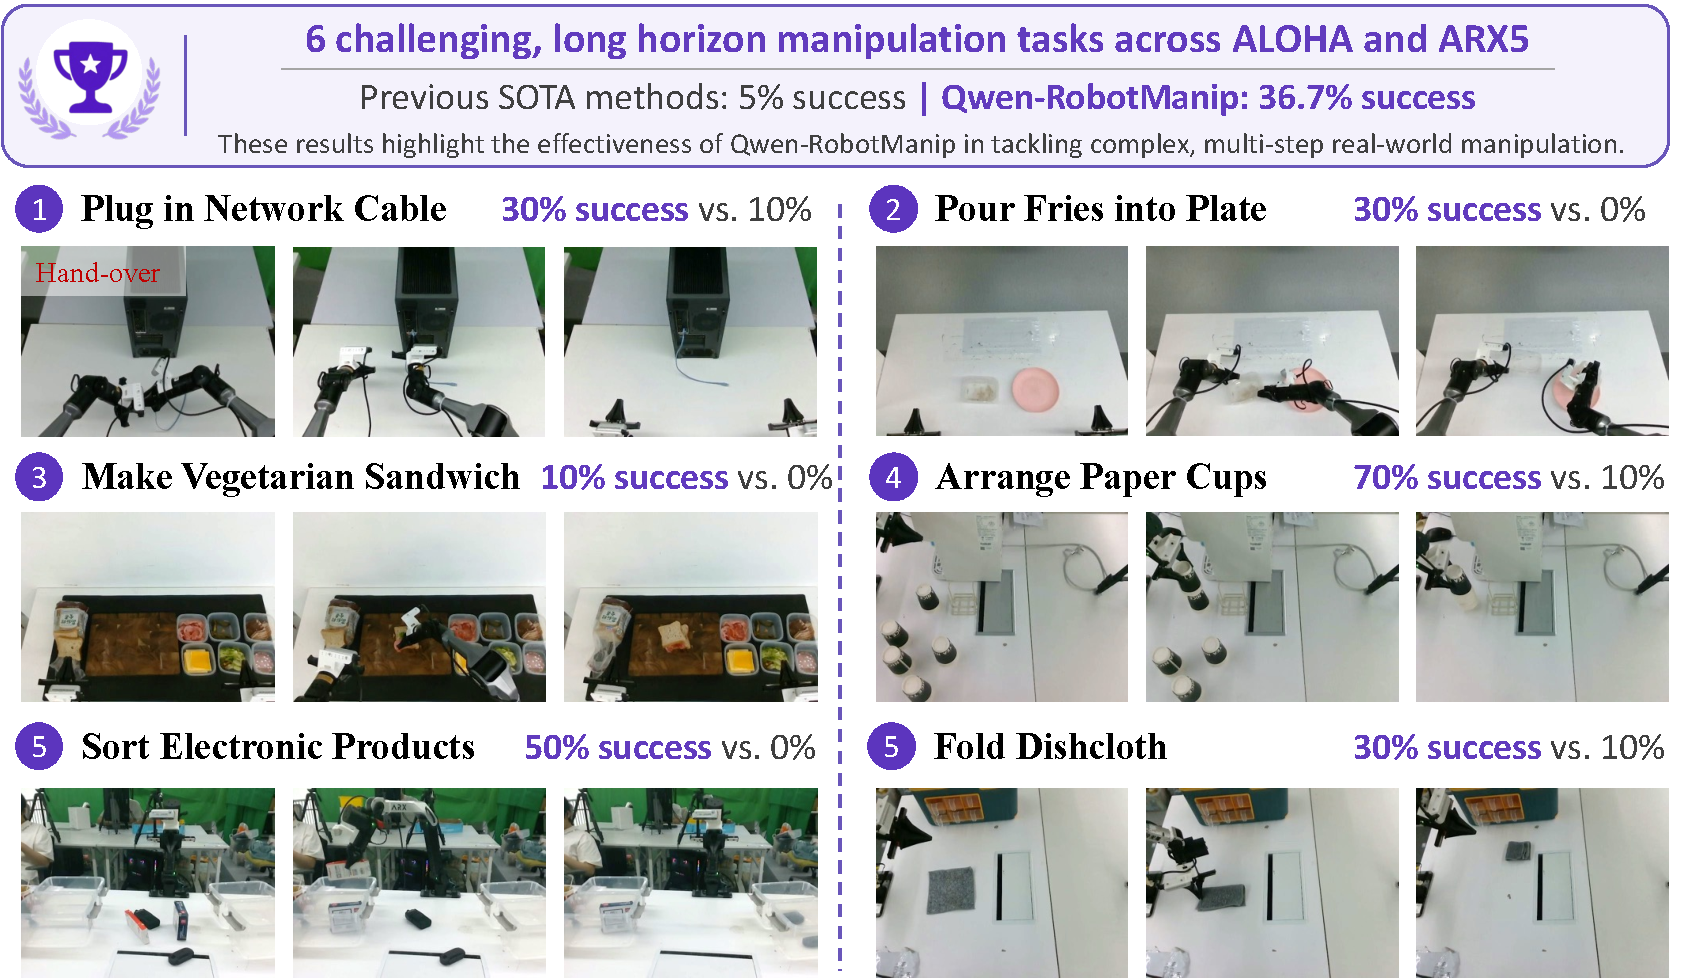
\includegraphics[width=0.95\textwidth]{figures/challenge_rc.pdf}
\caption{\textbf{\ours on six challenging long-horizon tasks from RoboChallenge Table30-v1}, spanning bimanual dexterous manipulation, sequential ingredient stacking, multi-object arrangement, and deformable object handling. Prior SOTA generalist methods achieve an average of 5\% success across these tasks. \ours achieves 36.7\%, with substantial margins on every task.}
\label{fig:challenging_tasks}
\end{figure}

% \textbf{Reliable execution of core skills.} On tasks requiring fundamental pick-and-place or single-step actuation (Figure~\ref{fig:core_skills}), such as \textit{turn on faucet} (100\%), \textit{stack bowls} (100\%), \textit{put cup on coaster} (100\%), \textit{set the plates} (100\%), \textit{arrange fruits in basket} (80\%), and \textit{move objects into box} (70\%) --- \ours achieves consistently high success rates across all four robot embodiments (ALOHA,
% ARX5, UR5, and Franka). These tasks serve as a basic sanity check for generalist policies: a model that cannot reliably grasp and place objects will inevitably fail at more complex behaviors. The fact that \ours solves these tasks at near-ceiling performance, despite being trained as a single multi-task policy per embodiment, confirms that generalist training does not sacrifice reliability on fundamental skills.

\textbf{Breakthrough on challenging tasks.}
The above three capabilities jointly enable \ours to achieve leading performance on several high-difficulty tasks where most generalist baselines fail entirely (see Figure~\ref{fig:challenging_tasks}). On the ALOHA platform, \textit{plug in network cable} (30\%) and \textit{pour fries into plate} (30\%) both demand precise bimanual coordination with fine posture adjustment, yet \ours is the only model achieving $\geq$30\% success rate. On \textit{make vegetarian sandwich} (10\%)---a long-horizon task requiring sequential ingredient stacking---\ours is the only model to achieve a non-zero success rate. On ARX5, spatial precision and self-correction combine to yield strong results on \textit{arrange paper cups} (70\%), \textit{sort electronic products} (50\%), and \textit{fold dishcloth} (30\%), outperforming the next-best method by 60, 40, and 20 percentage points respectively. These results demonstrate that cross-embodiment pre-training enables the interleaved acquisition of bimanual coordination, spatial precision, and self-corrective strategies, which collectively unlock complex manipulation skills that remain out of reach for existing generalist policies.

% \ours also achieves leading performance on several high-difficulty tasks where most generalist baselines fail entirely (Figure~\ref{fig:challenging_tasks}). On the ALOHA platform, \textit{plug in network cable} (30\%) and \textit{pour fries into plate} (30\%) both require bimanual coordination with precise posture adjustment, yet \ours is the only model achieving $\geq$30\% success rate. In contrast, baseline methods such as DM0 and pi0 frequently fail to coordinate both arms simultaneously, resulting in dropped objects or missed targets. On \textit{make vegetarian sandwich} (10\%) --- a long-horizon task involving sequential ingredient stacking --- \ours is the only model to achieve a non-zero success rate, while all other methods fail completely. A similar pattern emerges on ARX5: on \textit{arrange paper cups} (70\%), \textit{sort electronic products} (50\%), and \textit{fold dishcloth} (30\%), \ours substantially outperforms the next-best method by margins of 60, 40, and 20 percentage points respectively, while nearly all remaining baselines score zero. These results suggest that cross-embodiment pre-training enables the acquisition of complex manipulation skills --- including multi-object arrangement, deformable-object handling, and bimanual coordination.

\subsection{Ablation Study}

We ablate the core design choices of \ours: alignment strategies (state-action representation, in-context adaptation, architecture) and data recipes for scaling (human-to-robot synthesis, vision-language co-training). All variants within each group share identical training conditions at reduced pretraining scale; configurations may differ from the main results.
% We ablate the core design axes of \ours: alignment strategies (action space, embodiment prompt, and in-context adaptation), data recipes (egocentric human data and VL co-training), and network architecture. To enable efficient iteration, individual ablations are conducted at reduced pretraining scale; all compared variants within each study share identical training conditions.

\textbf{Action space alignment for data scaling. } A central promise of foundation models is that performance should improve predictably as training data grows. For vision-language-action models trained on heterogeneous cross-embodiment data, verifying this property requires careful design of how data from distinct robots is combined. If the action representations across embodiments are misaligned, simply adding more data may not yield increasing performance, because the model must spend capacity reconciling conflicting conventions rather than learning transferable manipulation structure.

To investigate this, we construct a controlled data-scaling experiment. Starting from the full cross-embodiment pre-training mixture, we create nested subsets at 1\%, 5\%, 10\%, 25\%, 50\%, and 100\% of the original dataset by sampling at the per-embodiment task level, ensuring that smaller subsets are strict subsets of larger ones. All models are evaluated on a fixed held-out OOD evaluation set spanning 15 embodiment types and 154 tasks that are entirely absent from any training set. For each data percentage and model variant, we report the best validation MSE achieved across all training checkpoints, measured in a unified action representation to ensure fair comparison across model variants.

\begin{figure}[!t]
    \centering
    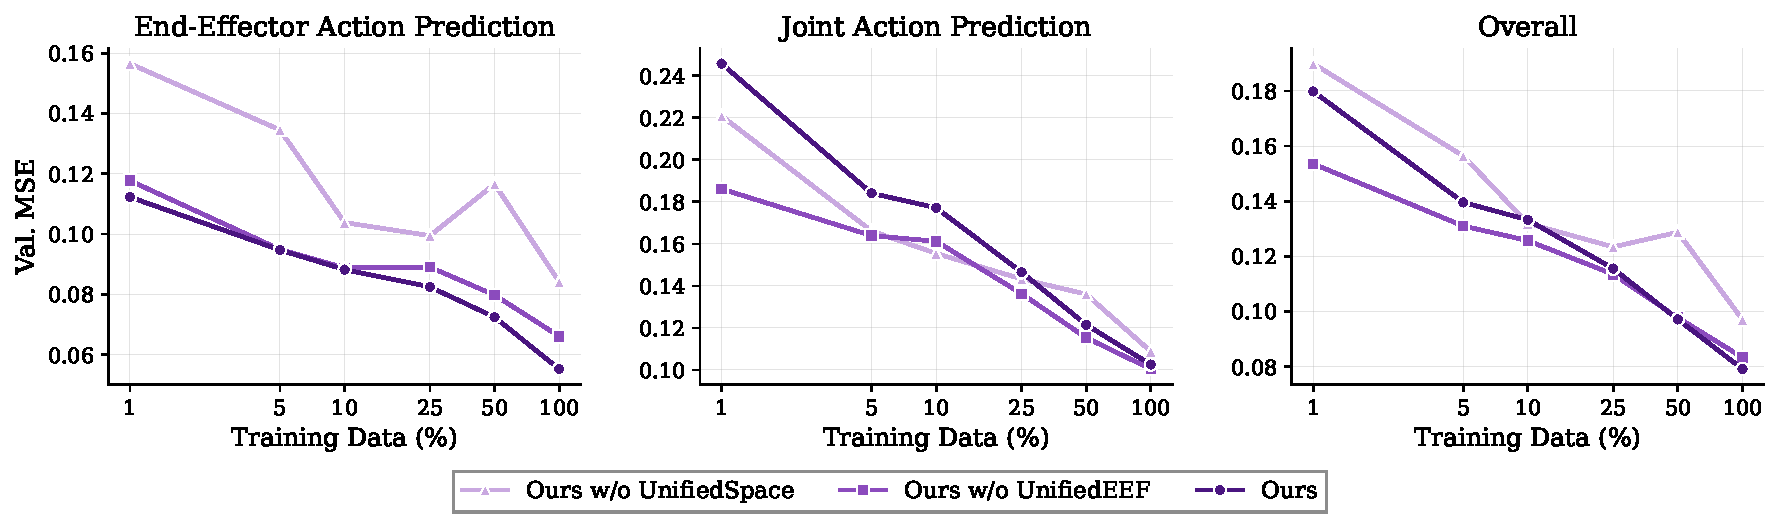
\includegraphics[width=1.0\linewidth]{figures/scaling_curves.pdf}
    \caption{\textbf{Data scaling curves for models with varied state and action representations,} evaluated on held-out validation datasets. Each point reports the best validation MSE across all training checkpoints for a given training data percentage.}
    \label{fig:scaling_curves}
\end{figure}

% \begin{table}[!t]
% \centering
% \caption{\textbf{Ablation study on action space alignment strategies} using out-of-distribution evaluation on RoboTwin-Clean2Rand with different execution modes.}
% \label{tab:ablation_action_space}
% \small
% \tabcolsep 5pt
% \begin{tabular}{l|cccc}
% \toprule & \textbf{Easy (joint)} & \textbf{Hard (joint)} & \textbf{Easy (eef)} & \textbf{Hard (eef)} \\
% \midrule
% \ours w/o UnifiedSpace   & 52.0 & 25.2 & 36.4 & 16.1  \\
% \ours w/o UnifiedEEF   & 58.7 & 39.2 & 49.0 & 33.0  \\
% \ours  & {68.1} & {50.2} & {72.5} & {56.6} \\
% \bottomrule
% \end{tabular}
% \end{table}

\begin{figure}[!t]
    \centering
    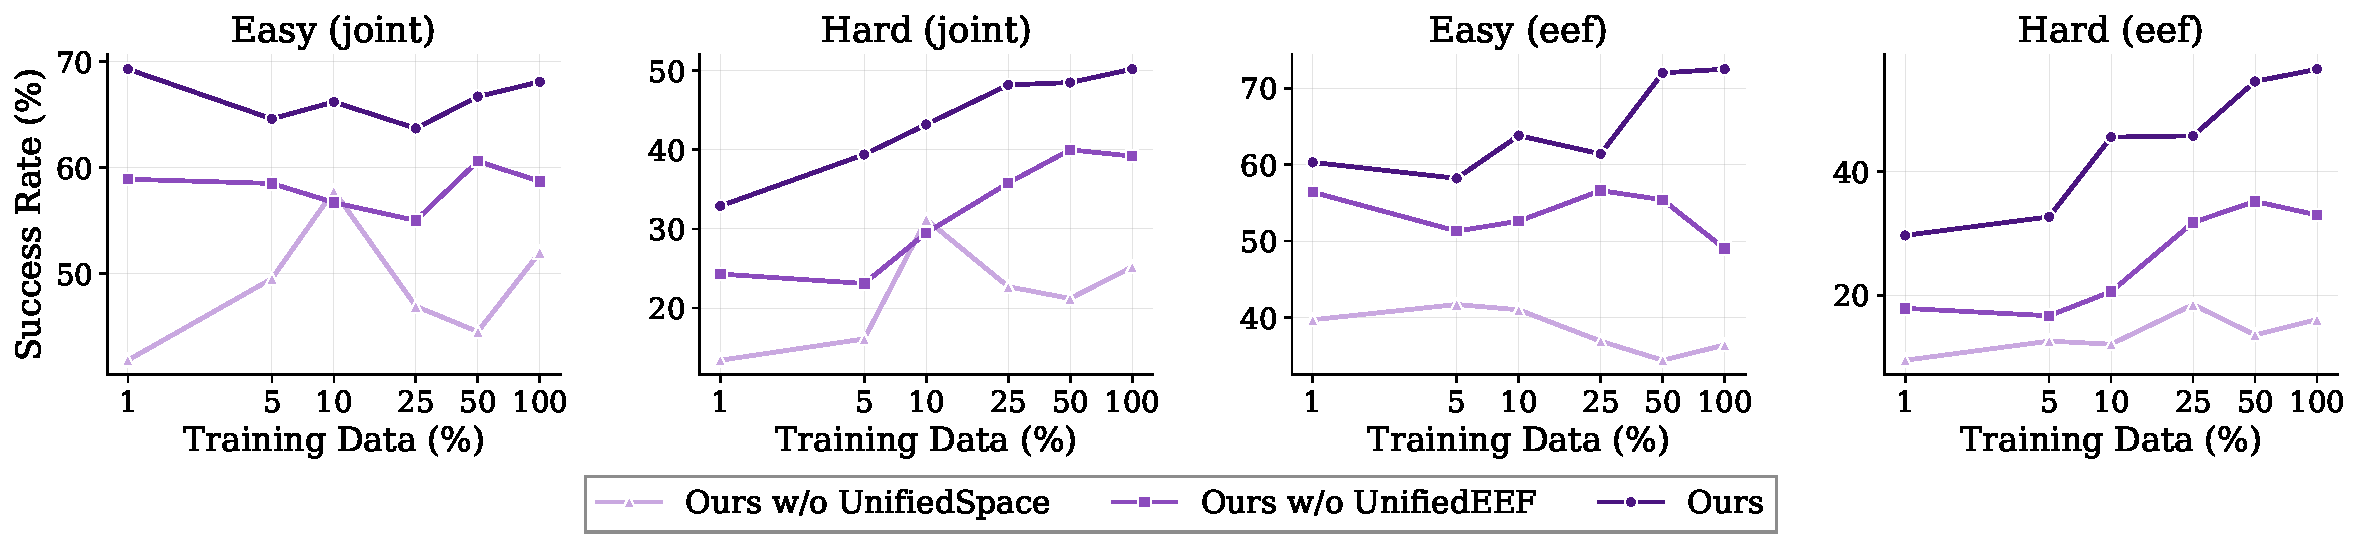
\includegraphics[width=1.0\linewidth]{figures/scaling_downstream.pdf}
     \caption{\textbf{Downstream performance on RoboTwin-C2R after fine-tuning models pre-trained with varied data percentages and action
  representations.} Each subplot reports success rate under a different control mode (joint or EEF) and evaluation setting (Easy or Hard).}
    \label{fig:scaling_curves_downstream}
\end{figure}

Figure~\ref{fig:scaling_curves} compares the scaling behavior of three action space designs. \textbf{Ours w/o UnifiedSpace} concatenates each embodiment's raw action fields and zero-pads to 80 dimensions without any cross-embodiment structural alignment. \textbf{Ours w/o UnifiedEEF} maps joints, end-effectors, grippers, and hands into semantically fixed positions within the 80-dimensional canonical vector (\cref{sec:unified_state_action}), with end-effector actions expressed as axis-angle deltas relative to the initial end-effector pose. \textbf{Ours} further unifies end-effector motion by expressing it as camera-frame delta poses (\cref{subsec:cam_delta_action}), grounding actions in the visual observation frame.

Models with unified representations, Ours w/o UnifiedEEF and Ours, both exhibit a clear data scaling law: their best validation MSE decreases approximately log-linearly with training data volume across the full 1\%--100\% range, confirming that with proper action-space alignment, scaling up cross-embodiment data consistently reduces OOD prediction error. Ours w/o UnifiedSpace, by contrast, shows notably different behavior. For action prediction on end-effector dimensions (Figure~\ref{fig:scaling_curves}, left), Ours w/o UnifiedSpace produces an unstable scaling curve with substantially higher MSE than the two unified variants. Ours achieves the lowest end-effector MSE on average, demonstrating that camera-frame alignment enables the most effective cross-embodiment transfer for end-effector control. 

% These offline prediction improvements translate directly into downstream task performance. Table~\ref{tab:ablation_action_space} reports success rates on RoboTwin-Clean2Rand after fine-tuning each pre-trained variant, evaluated under both joint-space and end-effector control modes. Action alignment consistently yields gains: Ours w/o UnifiedEEF improves over Ours w/o UnifiedSpace, and Ours achieves the best results in both the in-distribution Easy setting and the out-of-distribution Hard setting. A particularly notable pattern emerges in the control-mode comparison. The two variants without camera-frame EEF alignment perform worse under end-effector control than under joint control, while Ours achieves its highest success rates under end-effector control (72.5\% Easy, 56.6\% Hard), exceeding its own joint-control performance (68.1\% Easy, 50.2\% Hard). This reversal confirms that camera-frame alignment endows the model with strong generalization in end-effector control, a capability that is essential for cross-embodiment deployment where joint-level transfer is inherently limited by morphological differences.

These offline prediction improvements translate directly into downstream task performance. Figure~\ref{fig:scaling_curves_downstream} reports success rates on RoboTwin-C2R after fine-tuning each pre-trained variant on the RoboTwin Clean dataset for 80k steps, evaluated under four settings that combine two control modes (joint-space and end-effector) with two perturbation settings (Easy and Hard). Colors from dark to light correspond to progressively less aligned action representations: Ours, Ours w/o UnifiedEEF, and Ours w/o UnifiedSpace.
On the OOD Hard settings (second and fourth subplots), Ours exhibits a clear data scaling property: downstream success rate increases steadily as pretraining data grows from 1\% to 100\%, reaching 50.2\% (joint) and 56.6\% (EEF) at full scale. Ours consistently outperforms both ablated variants across all data percentages, while Ours w/o UnifiedEEF and Ours w/o UnifiedSpace show noisier scaling curves with less consistent improvement. In contrast, on the in-distribution Easy settings (first and third subplots), none of the three variants shows a clear upward trend with increasing pretraining data. This corroborates the finding in \cref{subsec:are_std_bench_enough} that standard in-distribution evaluation fails to capture the benefits of large-scale pretraining, and that OOD evaluation is needed to reveal the genuine scaling behavior. 
A further notable pattern emerges in the control-mode comparison: Ours achieves comparable or higher success rates under EEF control than under joint control on both Easy and Hard, while both ablated variants show the opposite trend. This confirms that camera-frame alignment produces a strong EEF-space policy, a capability essential for cross-embodiment transfer.

\textbf{Ablation study on embodiment prompt design and in-context policy adaptation.}
We ablate the embodiment prompt design and in-context policy adaptation mechanism using an early checkpoint of \ours trained on a smaller data subset, evaluated on RoboTwin-Clean2Rand under out-of-distribution settings. Results are reported in Table~\ref{tab:ablation_prompt_context}.

\begin{table}[!t]
\centering
\caption{\textbf{Ablation study on embodiment prompt design and in-context policy adaptation.} Out-of-distribution evaluation on RoboTwin-Clean2Rand (joint). The speed is set to 500.}
\label{tab:ablation_prompt_context}
\small
\tabcolsep 5pt
\begin{tabular}{l|cccc|ccc}
\toprule
& \textbf{Emb. Tag} & \textbf{FPS} & \textbf{Context} & \textbf{Denoise Steps} & \textbf{Easy} & \textbf{Hard} & \textbf{Avg} \\
\midrule
\ours w/o UnifiedEEF        & \texttimes & \texttimes & \texttimes & 4 & 71.2 & 54.2 & 62.7 \\
+ Soft-Prompt        & soft       & \texttimes & \texttimes & 4 & 70.2 & 52.1 & 61.2 \\
+ Language Prompt    & lang.      & 15 & \texttimes & 4 & 71.7 & 55.1 & 63.4 \\
+ Structure Prompt   & \checkmark & 15         & \texttimes & 4 & 73.4 & 58.3 & 65.9 \\
% + Structure Prompt   & \checkmark & 30         & \texttimes & 4 & 73.5 & 57.3 & 65.4 \\
\midrule
\ours-Context        & \checkmark & 15 & \checkmark & 4  & 72.1 & 54.4 & 63.3 \\
\ours-Context        & \checkmark & 15 & \checkmark & 10 & 80.1 & 61.6 & 70.9 \\
\ours-Context        & \checkmark & 15 & \checkmark & 20 & 79.8 & 62.1 & 71.0 \\
\bottomrule
\end{tabular}
\end{table}

On the prompt side, encoding embodiment identity as a learnable soft prompt slightly degrades performance relative to the na\"ive baseline. A natural language prompt recovers this and yields a modest gain, suggesting that semantic embodiment labels carry some useful signal, but the improvement remains small, indicating that coarse identity information alone is insufficient to meaningfully adjust behavior across embodiments. The structured embodiment prompt, which additionally conditions the model on the temporal properties of the episode via the FPS field, produces consistent improvements of 2.2-3.2 points.
% A fine-grained analysis across fps values of 15, and 30 and speed values of 500, 1000, and 1500 shows that clean-setting performance is largely insensitive to these fields, while OOD performance peaks when they match the training distribution of the RoboTwin data, namely fps 15 and speed 500 (indicating a 500-timestep episode budget). 
The structured prompt provides robustness under distribution shift rather than overfitting to a fixed temporal configuration, but is most effective when its fields faithfully reflect the deployment context.

Prompt-level conditioning, however, captures only static episode metadata. The in-context policy adaptation mechanism introduces dynamic intra-episode information in the form of a single historical observation-action chunk, enabling the model to observe the robot's actual behavioral dynamics rather than relying on coarse category labels. Without context, the policy action distribution is smooth and 4 denoising steps is already sufficient, producing stable behavior with no signs of jitter. Introducing execution history increases the complexity of the action distribution, causing the policy to produce jittery motion at the same 4-step budget, which largely negates the benefit of the context signal and yields performance near the na\"ive baseline. Increasing the denoising budget to 10 steps resolves the instability and unlocks the full benefit of the context mechanism, reaching 70.9 average and a 5.0-point improvement over the structure prompt baseline, a margin that dwarfs the contribution of any prompt design variant. Further increasing to 20 steps yields no additional gain. These results support the view that in-context history functions as an implicit embodiment identifier reflecting intra-episode kinematic signatures rather than as episodic memory, and that this signal is qualitatively distinct from what static prompt conditioning can provide, provided the action head has sufficient capacity to decode it faithfully. 

We do note one practical limitation observed in real-robot deployment: at the start of an episode, the context consists entirely of zero-padded placeholders, and the model, having learned to condition on quiescent history, tends to hesitate before initiating motion. We therefore release both the context-conditioned and context-free variants of \ours, allowing users to select appropriate configuration depending on whether rapid response or richer intra-episode adaptation is the priority.

% Ablation on structured prompt
% baseline: (1) pre-train without prompt (QwenGR00Tv1) + post-train without prompt, (2) pre-train with prompt + post-train with prompt, 

% Test time steerability.
% fps
% speed robustness

% Only on Robotwin Clean2Rand

% context:
% (4) dual mode

% Another one experiment on LIBERO-Plus but only have no context and our unified mode experiment

%[low-p] 2. Ablation on context length
%baseline: context length 1, context length 3

% \textbf{Vision-language co-training.}
% \textbf{Effect of VL data co-training in pre-training.} We ablate the role of VL data during the pre-training stage by comparing our full model against a variant pre-trained without any VL data mixture (Table~\ref{tab:vl_data_in_pretraining_ablation}). On LIBERO and LIBERO-Plus, removing VL data leads to modest drops of 0.9 and 1.2 points, respectively, as these benchmarks are relatively simple for VLA model. However, on the more challenging RoboTwin benchmarks, the gap widens significantly: RoboTwin-E2H (easy) drops by 6.7 points and RoboTwin-E2H (hard) by 8.2 points, indicating that VL co-training becomes increasingly important as task diversity and scene complexity grow. We attribute this to the complementary roles of different VL data subsets: general VL data mitigates catastrophic forgetting of the VLM's broad perceptual and linguistic capabilities; spatial grounding and reasoning data strengthens spatial and scene understanding for precise manipulation; and embodied-centric data aligns the VLM's representations with the semantic structure of manipulation tasks. Together, they produce VLM's representations better suited for downstream action expert alignment.

\textbf{Ablation study on human-to-robot synthetic data.}
To isolate the contribution of egocentric human data, we compare three pretraining configurations on RoboTwin-Clean2Rand (eef) and LIBERO-Plus at a fixed 7:3 robot-to-auxiliary ratio (Tables~\ref{tab:h2r_robotwin} and~\ref{tab:h2r_libero}): \textbf{Robot-only} uses robot data only; \textbf{+Ego} mixes in raw egocentric data; \textbf{+H2R} replaces the raw data with pipeline-synthesized robot demonstrations from the same ego sources. 
All three share identical training steps, hyperparameters, and finetuning data, so any performance difference is attributable solely to the auxiliary data source.

On RoboTwin-Clean2Rand, the Hard setting---where all perturbations are applied simultaneously---shows the clearest separation: +H2R reaches 58.7\%, a +4.0 gain over Robot-only (54.7\%) and +3.7 over +Ego (55.0\%). 
Per-dimension gains are consistent, with the largest on Light (+3.0) and Height (+3.2), where the varied camera perspectives and lighting in ego data naturally augment robustness. 
The Easy setting also sees a modest improvement (72.9 $\to$ 73.4 $\to$ 74.2).

On LIBERO-Plus, +H2R raises the average success rate from 87.1\% to 89.0\%. 
The Camera dimension shows the largest improvement (+7.2 over Robot-only, 72.8 $\to$ 80.0), as egocentric data provides diverse viewpoint coverage that robot-only data lacks. 
The Robot dimension also benefits (+2.0), suggesting that the diverse manipulation trajectories in H2R data improve robustness to initial pose variation.
The monotonic Robot-only $\to$ +Ego $\to$ +H2R progression across both benchmarks confirms that raw ego data contributes through visual diversity, while the H2R pipeline unlocks additional gains via action and visual alignment.

\begin{table}[!t]
\centering
\caption{\textbf{Human2Robot ablation on RoboTwin-Clean2Rand (eef).}}
\label{tab:h2r_robotwin}
\small
\tabcolsep 3pt
\begin{tabular}{lcccccc}
\toprule
& \textbf{Easy} & \textbf{Background} & \textbf{Light} & \textbf{Clutter} & \textbf{Height} & \textbf{Hard} \\
\midrule
\ours (robot-only) & 72.9 & 70.4 & 70.3 & 57.2 & 67.8 & 54.7 \\
\ours (+ego) & 73.4 & 70.6 & 71.7 & \textbf{59.2} & 70.2 & 55.0 \\
\ours (+h2r) & \textbf{74.2} & \textbf{71.4} & \textbf{73.3} & 58.1 & \textbf{71.0} & \textbf{58.7} \\
\bottomrule
\end{tabular}
\end{table}

\begin{table}[!t]
\centering
\caption{\textbf{Human2Robot ablation on LIBERO-Plus.}}
\label{tab:h2r_libero}
\small
\tabcolsep 3pt
\begin{tabular}{lcccccccc}
\toprule
& \textbf{Camera} & \textbf{Robot} & \textbf{Language} & \textbf{Light} & \textbf{Background} & \textbf{Noise} & \textbf{Layout} & \textbf{Total} \\
\midrule
\ours (robot-only) & 72.8 & 78.2 & 88.7 & 97.5 & 97.6 & 95.4 & \textbf{85.4} & 87.1 \\
\ours (+ego) & 77.7 & 79.0 & 88.5 & \textbf{98.8} & \textbf{98.7} & \textbf{97.3} & 84.9 & 88.4 \\
\ours (+h2r) & \textbf{80.0} & \textbf{80.2} & \textbf{89.3} & 98.5 & 98.2 & 96.6 & 85.2 & \textbf{89.0} \\
\bottomrule
\end{tabular}
\end{table}

\textbf{Effect of VL data co-training during pre-training.} 
We study the role of VL data in the pre-training stage by comparing our full model with a variant pre-trained without any VL data mixture (Table~\ref{tab:vl_data_in_pretraining_ablation}). On LIBERO and LIBERO-Plus, removing VL data causes relatively small drops of 0.9 and 1.2 points, respectively. In contrast, the performance degradation is much larger on the more challenging RoboTwin benchmarks: RoboTwin-Clean2Rand (easy) drops by 6.7 points, RoboTwin-Clean2Rand (hard) by 8.2 points, and RoboTwin-IF by 7.0 points. This trend indicates that VL co-training becomes increasingly important as task diversity, scene complexity, and distribution shift grow.

We attribute these gains to the complementary benefits of different VL data sources. General-domain VL data helps preserve the VLM's broad perceptual and linguistic capabilities, reducing catastrophic forgetting during VLA training. Spatial grounding and reasoning data improves the model's ability to localize objects, understand spatial relations, and reason over complex scenes, which is crucial for precise manipulation. Embodied-centric VL data further aligns the VLM's representations with the semantic structure of embodied tasks. Together, these data sources yield VLM representations that are better suited for downstream alignment with the action expert.

\begin{table}[!t]
\centering
\caption{\textbf{Ablations on VL data co-training in the pre-training and post-training stage.} By default, \ours is pre-trained with VL data and post-training without it. (``RT'' is the abbreviation of ``RoboTwin''.)}
\label{tab:vl_data_in_pretraining_ablation}
\small
\tabcolsep 2.5pt
\begin{tabular}{lccccc}
\toprule
& \textbf{LIBERO} & \textbf{LIBERO-Plus} & \textbf{RT-C2R (easy)} & \textbf{RT-C2R (hard)} & \textbf{RT-IF} \\
\midrule
\ours & \textbf{99.1} & 90.1 & 73.2 & \textbf{62.6} & 71.6 \\
\quad - without VL data in pre-training & 98.2 & 88.9 & 66.5 & 54.4 & 64.6 \\
\quad - with VL data in post-training & 98.6 & \textbf{91.4} & \textbf{74.0} & 62.5 & \textbf{73.1} \\
\bottomrule
\end{tabular}
\end{table}

% The improvement of VL co-training Pre-train (v1 VL co-training vs. previous v1 version): SFT on RoboTwin and libero.

% Post-train: SFT on RoboTwin clean, eval on RoboTwin clean/randomized/if/Clean2Rand; SFT on libero, eval on libero/libero-plus; real-world robot?

% As shown in Table~\ref{tab:robotwin_if_cotrain_ablation}, adding VL data during post-training yields substantial improvements on RoboTwin-IF across four out of five tasks, with the most prominent gains on Place-Relative (+32) and Pick-Diverse (+25), followed by Operated-Tabletop (+14) and Operated-Stapler (+5), while Operated-Mic-Drawer remains comparable (-3, within noise). 



% \begin{table}[!t]
% \centering
% \caption{Instruction-following evaluation on RoboTwin-IF (Ablations on mixed post-training strategies).}
% \label{tab:robotwin_if_cotrain_ablation}
% \small
% \tabcolsep 2.5pt
% \begin{tabular}{lcccccc}
% \toprule
% & \textbf{Pick} & \textbf{Place} & \textbf{Ope.-Mic-Drawer} & \textbf{Ope.-Stapler} & \textbf{Ope.-Tabletop} \\
% \midrule
% \ours (eef) & 65 & 26 & 46 & 78 & 76 \\
% \quad + VL data post-training & 90 & 58 & 43 & 83 & 90 \\
% \quad + sim VLA data post-training & - & - & - & - & - \\
% \quad + rebalance verb VLA data post-training & - & - & - & - & - \\
% \bottomrule
% \end{tabular}
% \end{table}


% \textbf{Mixed post-training strategies. \orange{(zixing, linpei, yiyang)}}


% \orange{2 paragraphs: vl data; vla data}
% evaluate on robotwin-if \orange{add sim data; rebalance verb data; add vl data}

%\orange{anzhe}
% Like: Self-attention vs. cross-attention: the latter improves visual robustness?
% \begin{itemize}
%     \item per layer cross/self attention (pi-style)
%     \item last layer cross/self attention
%     \item last layer cross attention
% \end{itemize}
% Only on Libero-plus. No obvious advantage on Robotwin.
% We design three architectures:

\begin{figure}[!t]
    \centering
    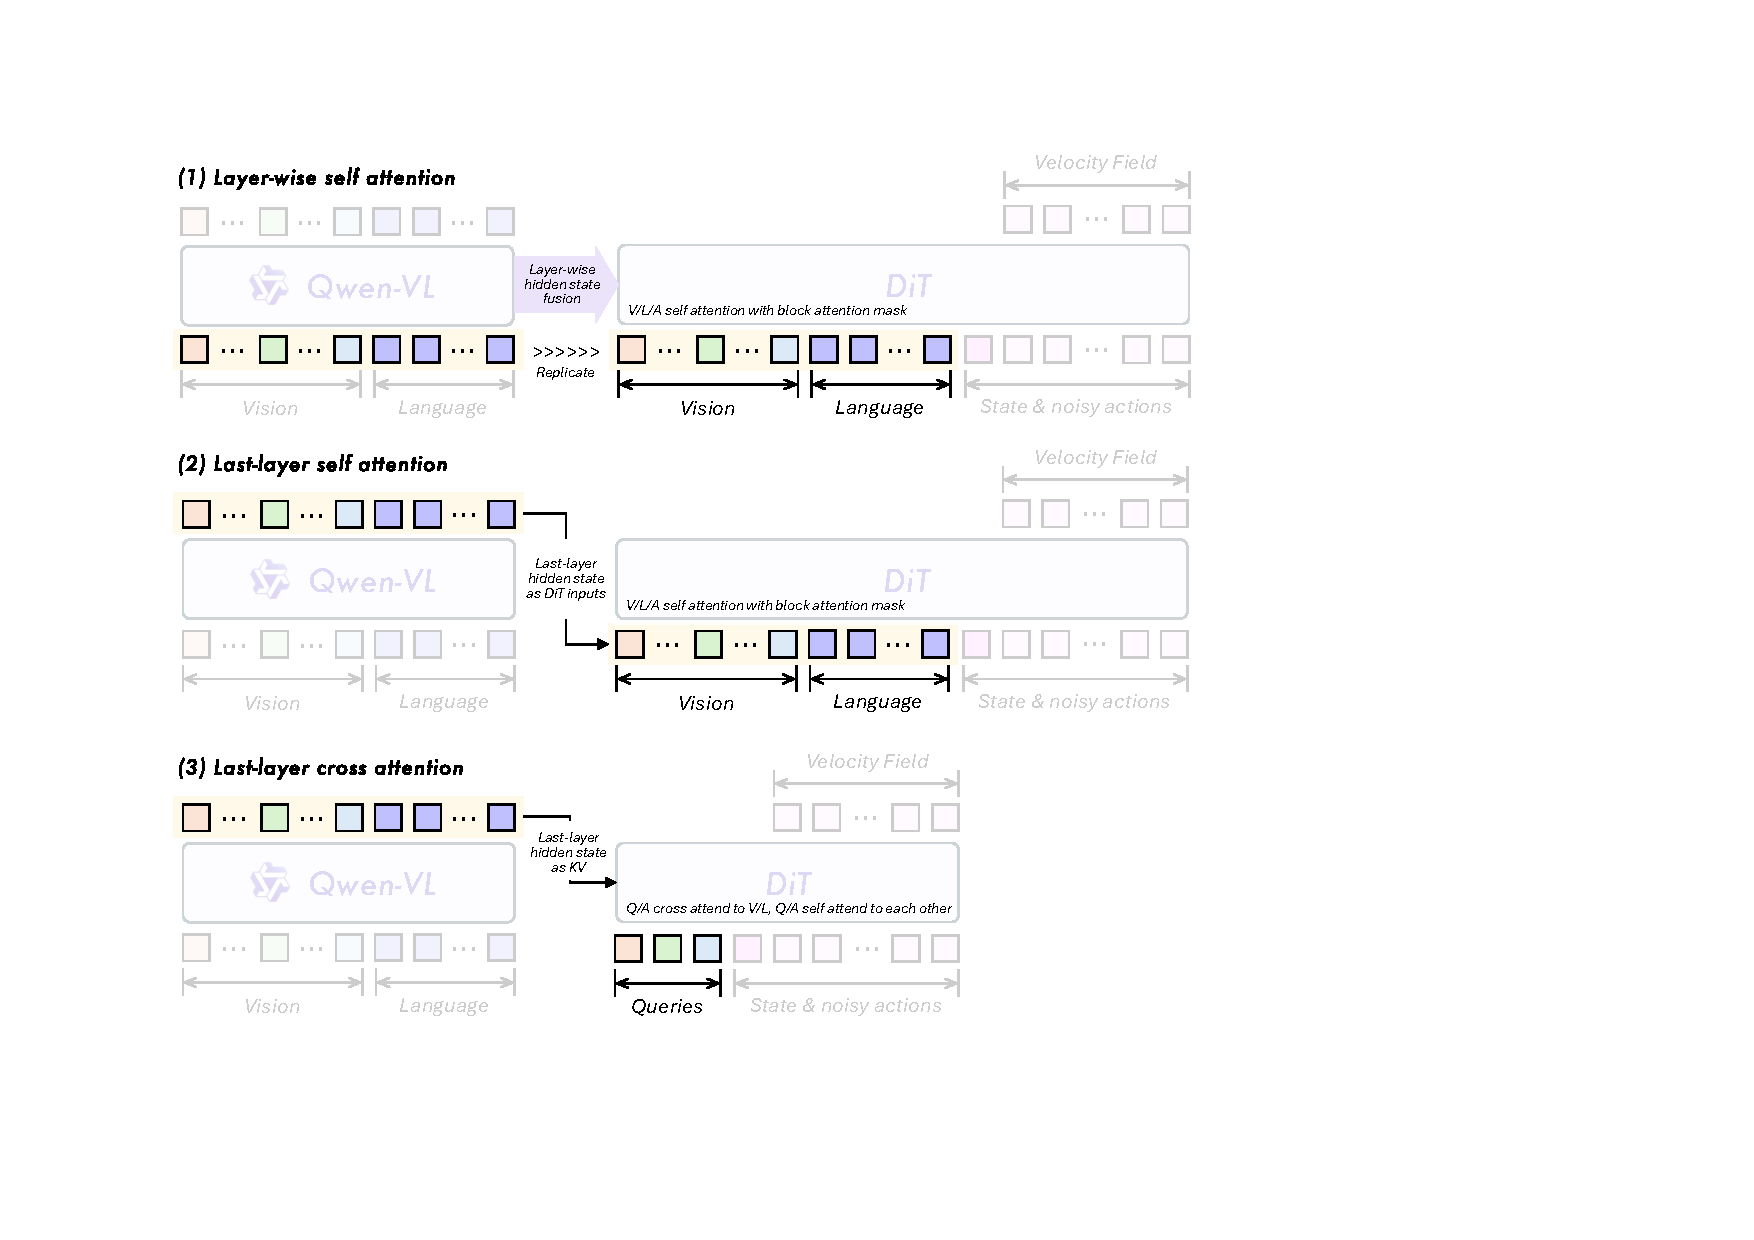
\includegraphics[width=0.8\linewidth]{figures/ablate-nn-arch.pdf}
    \caption{\textbf{Ablation study of model architecture variants.} }
    \label{fig:ablate-nn-arch}
\end{figure}


\textbf{Architecture design. }
We conduct ablation experiments on three network architecture variants (Figure~\ref{fig:ablate-nn-arch}):
\begin{enumerate}[leftmargin=*,topsep=2pt,itemsep=1pt]
    \item The first variant replicates the VLM's vision and language hidden states as input to the DiT, and employs a pure self-attention architecture within the DiT. After each self-attention layer in the DiT, the vision and language features are fused with the corresponding per-layer vision and language features from the VLM via a weighted residual combination.
    \item The second variant feeds only the VLM's \emph{last-layer} hidden states into the DiT. The DiT likewise uses a pure self-attention architecture, but without any per-layer feature fusion with the VLM's intermediate representations.
    \item The third variant introduces a small set of learnable query tokens~\citep{ICLR2024Registers} that act as condensed proxies for the VLM's vision and language tokens. 
    These query tokens are concatenated with the state and action tokens; all tokens jointly cross-attend to the VLM's last-layer hidden states and self-attend among themselves. The query tokens' outputs are discarded after processing.
    % These query tokens interact with the VLM's last-layer hidden states through cross-attention, and simultaneously interact with the state and action tokens through self-attention.
\end{enumerate}

All three variants are pretrained exclusively on robot data and then fine-tuned on the LIBERO dataset. During both pretraining and fine-tuning, we exclude the structured embodiment prompt (retaining only the original task instruction), ECoT data, and in-context policy adaptation, isolating the camera-frame delta pose representation as the sole alignment design retained in this comparison.


The results are presented in Table~\ref{tab:libero_plus_diff_arch}. On LIBERO-Plus, the third variant (last-layer cross-attention) achieves the highest average success rate (87.5\%) while incurring the lowest computational cost, as it avoids both per-layer feature fusion and storing the full set of VLM vision-language tokens in the DiT. The pure self-attention architectures, whether with per-layer or last-layer fusion, do not exhibit a clear advantage for vision-language-action feature interaction. We therefore adopt the third architecture in all subsequent experiments.

\begin{table}[!t]
\centering
\caption{\textbf{Evaluation on LIBERO-Plus for different network architecture variants.}}
\label{tab:libero_plus_diff_arch}
\small
\tabcolsep 3pt
\begin{tabular}{lcccccccc}
\toprule
& \textbf{Camera} & \textbf{Robot} & \textbf{Language} & \textbf{Light} & \textbf{Background} & \textbf{Noise} & \textbf{Layout} & \textbf{Total} \\
\midrule
layer-wise self attention & 74.5 & 74.3 & 86.8 & 98.6 & 96.0 & 94.9 & 86.1 & 86.4 \\
last-layer self attention & 75.5 & 71.4 & 87.2 & 98.3 & 98.9 & 96.1 & 88.1 & 87.0 \\
last-layer cross attention & 76.9 & 73.4 & 86.9 & 98.9 & 97.7 & 97.3 & 87.3 & {\textbf{87.5}} \\
\bottomrule
\end{tabular}
\end{table}

% \textbf{Baselines (train on robotwin-clean, for OOD test)}: \textbf{dream-zero}, fast-wam, lingbot-vla, lingbot-va, wall-oss

\subsection{New Features after Alignment}
%\subsubsection{Post-training with VL Data}

\subsubsection{Post-train with VL Data and VLA Data in Pre-training Recipe}
\label{sec:mixposttrain}

\textbf{Setting 1: Post-training with VL data co-training.} In our main experiments, to match the standard fine-tuning setting, VL data is used only during pre-training and excluded from post-training. Here, we further investigate whether incorporating VL data into the post-training stage can improve generalization.

As shown in Table~\ref{tab:vl_data_in_pretraining_ablation} (see ``- with VL data in post-training''), adding VL data during post-training leads to improved performance on several benchmarks. In particular, it improves LIBERO-Plus from 90.1 to \textbf{91.4}, RoboTwin-Clean2Rand (easy) from 73.2 to \textbf{74.0}, and RoboTwin-IF from 71.6 to \textbf{73.1}, while the performance on RoboTwin-Clean2Rand (hard) remains nearly unchanged (62.6 vs.\ 62.5). These results suggest that post-training with VL data is particularly helpful for out-of-distribution generalization.

A closer analysis shows that the gain is most evident on \textit{language-related generalization benchmarks}. For example, on LIBERO-Plus, the success rate under language perturbations increases from 86.9\% for \ours to 93.9\% when VL data is included during post-training. Similarly, on RoboTwin-IF, post-training with VL data improves the success rate from 76\% to 81\% on the ``Pick-Diverse-Object'' suite. In contrast, RoboTwin-Clean2Rand (hard) keeps the instructions fixed and instead introduces visual distractors, background changes, and lighting variations, so the benefit of VL data is less pronounced in this setting.

% In contrast, RoboTwin-Clean2Rand (hard) keeps the instruction fixed and instead introduces more visual distractors, background changes, and lighting variations. The relatively smaller gain on RoboTwin-Clean2Rand therefore suggests that co-training VL data in post-training mainly benefits language understanding and instruction robustness, while offering limited improvements for visual robustness under substantial environmental changes.

We attribute these improvements to better preservation of the base VLM's foundational capabilities. Fine-tuning solely on action prediction can erode the pretrained VLM's language understanding and visual grounding abilities due to catastrophic forgetting, thereby weakening its capacity to interpret novel instructions at test time. In contrast, mixing VL data into post-training helps maintain these capabilities, enabling the model to better parse unseen instructions, ground referring expressions to visual entities, and translate linguistic intent into appropriate actions.

\begin{figure*}[!t]
  \centering
  
  % 左侧 Figure: pi0.5 mixposttrain
  \begin{minipage}{0.48\textwidth}
    \centering
    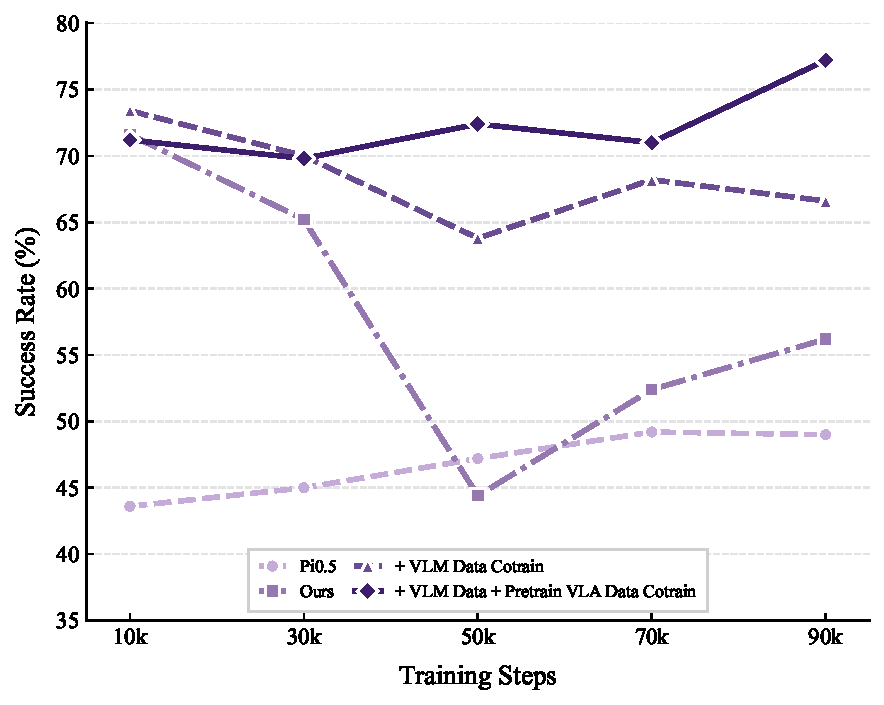
\includegraphics[width=0.85\linewidth]{figures/mixposttrain.pdf}
    \caption{
      \textbf{Performance comparison under different proportions of training data in RoboTwin-IF.}
      We report the score at 10k, 30k, 50k, 70k, and 90k training steps.
      Compared with the baseline \texttt{pi05}, our method benefits from
      incorporating VLM data and further improves when co-training with both
      VLM data and VLA pretraining data.
    }
    \label{fig:mixposttrain}
  \end{minipage}\hfill
  % 右侧 Figure: Qwen-RobotManip ablation
  \begin{minipage}{0.48\textwidth}
    \centering
    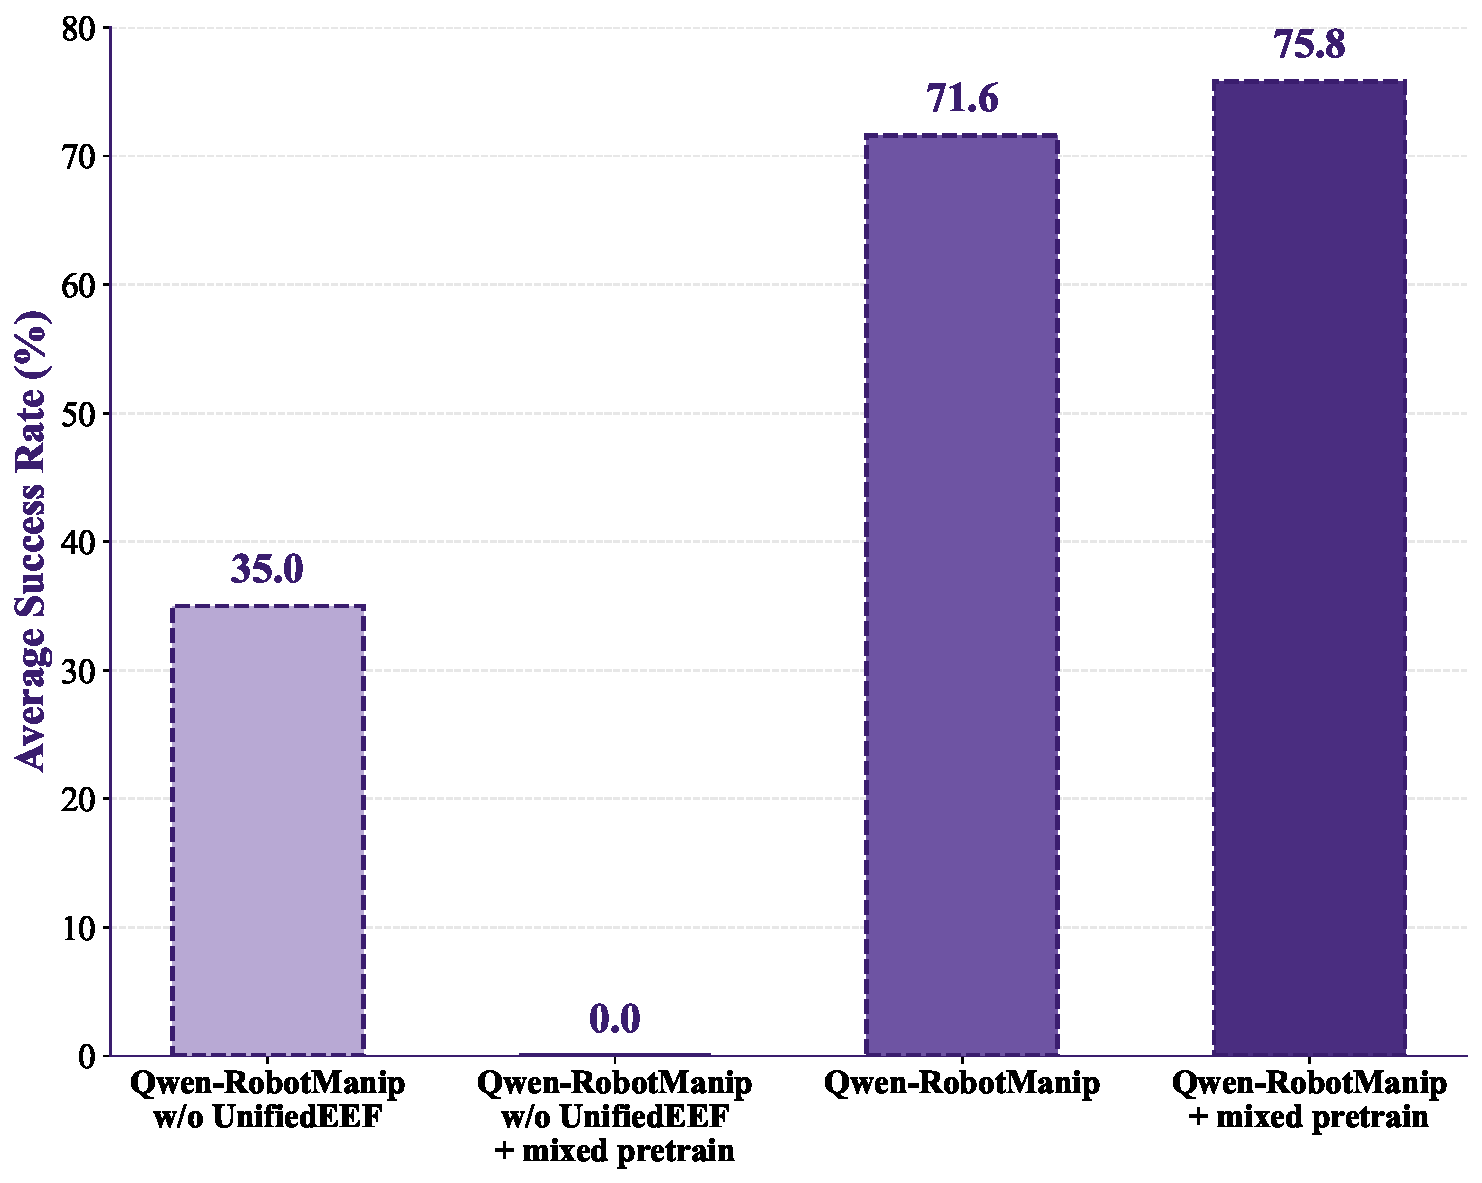
\includegraphics[width=0.85\linewidth]{figures/mixedposttrain.pdf}
    \caption{
      \textbf{Instruction-following success rates across configurations.} The chart highlights the critical necessity of the UnifiedEEF module, showing severe degradation without it (35.0\%) and total failure when combined with mixed pretraining (0.0\%). The optimal configuration utilizes both the base architecture and mixed pretraining (75.8\%).
    }
    \label{fig:mixedposttrain_ablation}
  \end{minipage}
  
\end{figure*}


% \begin{figure}[!t]
%   \centering
%   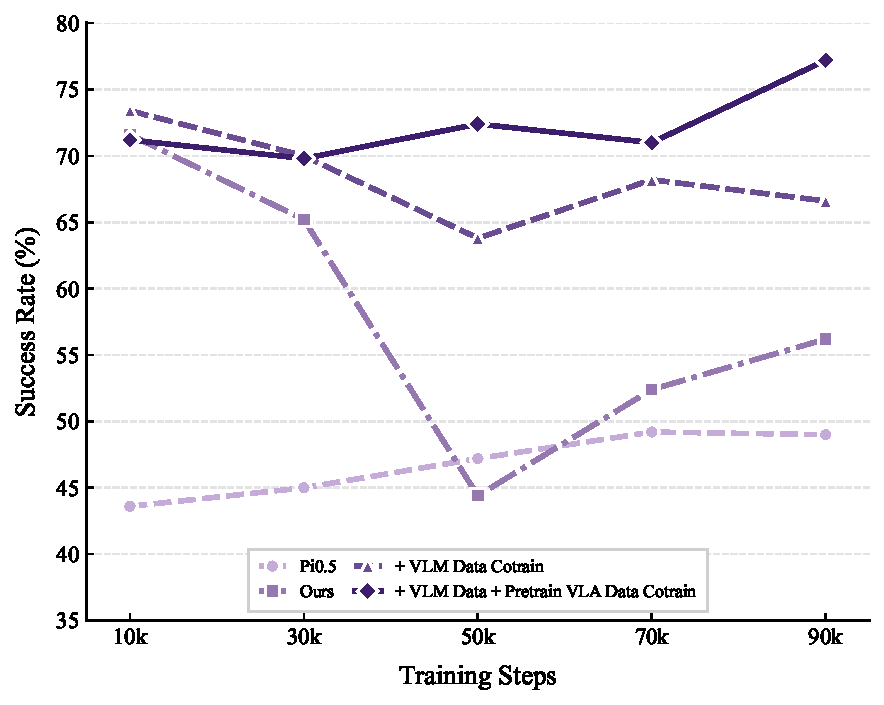
\includegraphics[width=0.45\linewidth]{figures/mixposttrain.pdf}
%   \caption{
%   \textbf{Performance comparison under different proportions of training data.}
%   We report the score at 10k, 30k, 50k, 70k, and 90k training steps.
%   Compared with the baseline \texttt{pi05}, our method benefits from
%   incorporating VLM data and further improves when co-training with both
%   VLM data and VLA pretraining data.
%   }
%   \label{fig:mixposttrain}
% \end{figure}

% \begin{table}[htbp]
% \centering
% \small
% \begin{tabular}{l|ccccc|c}
% \toprule
%  & \textbf{Pick-Diverse} & \textbf{Place-Rel.} & \textbf{Place-Rel.} & \textbf{Place-Rel.} & \textbf{Ope.-Table} & \textbf{Average} \\
% \midrule
% \textsc{Qwen-RobotManip}-Na\"ive & 25.0 &  7.0 & 41.0 & 47.0 & 55.0 & 35.0 \\
% + Pretrain VLA Data              &  0.0 &  0.0 &  0.0 &  0.0 &  0.0 &  0.0 \\
% \midrule
% Ours                             & 76.0 & \textbf{61.0} & \textbf{44.0} & 89.0 & 88.0 & 71.6 \\
% + VLM data                       & 81.0 & \textbf{61.0} & 42.0 & 91.0 & 92.0 & 73.4 \\
% + VLM data + Pretrain VLA Data   & \textbf{90.0} & \textbf{61.0} & 40.0 & \textbf{93.0} & \textbf{95.0} & \textbf{75.8} \\
% \bottomrule
% \end{tabular}
% \caption{\textbf{Instruction-following evaluation on RoboTwin-IF.} This experiment aims to evaluate the multi-task instruction-following proficiency and generalization performance of different models and data mixtures. Models are fine-tuned on RoboTwin Clean dataset and evaluated with held-out unseen instruction templates.}
% \label{tab:posttrain_ablation}
% \end{table}

\textbf{Setting 2: Post-training with VL and auxiliary VLA data co-training.} When transferring VLA models to a specific downstream domain via post-training such as a novel simulation environment, robot embodiment, or operational scene—it is standard practice to rely exclusively on clean, domain-specific datasets. However, this paradigm introduces a prominent bottleneck in VLA adaptation: severe domain overfitting. In most scenarios, rather than acquiring genuine, generalizable instruction-following capabilities, the model essentially memorizes the specific scene dynamics. Leveraging our proposed unified action space representation, we introduce a mixed post-training strategy to systematically enhance the model's generalization capacity within the target domain. Specifically, during the curation of the post-training dataset, we augment the target-domain data by integrating a mixture of general Vision-Language (VL) data and pre-training VLA data. Crucially, this mixed-data approach effectively mitigates overfitting without compromising the model's low-level physical execution proficiency in the target domain.

Specifically, our augmented dataset comprises two primary categories. The first consists of Vision-Language (VL) data, predominantly derived from standard Vision-Language Model (VLM) training corpora, encompassing tasks such as object detection, spatial pointing, and trajectory prediction. The second category entails VLA data, which aggregates trajectories from auxiliary simulators alongside large-scale, real-world demonstrations from morphologically similar embodiments. To facilitate effective cross-embodiment transfer, we align and optimize this auxiliary VLA data within the highly transferable end-effector (EEF) action space.

We evaluate our approach on RoboTwin-IF, the Out-of-Distribution benchmark within our target domain, RoboTwin. As shown in Figure~\ref{fig:mixposttrain}, when fine-tuning exclusively on the domain-specific RoboTwin-Clean dataset, our model initially achieves performance that significantly surpasses that of $\pi_{0.5}$. However, as the number of training steps increases, severe overfitting emerges, leading to a progressive performance decay on the RoboTwin-IF evaluation. By integrating VL data (accounting for 10\% of the training mixture), both the instability of the peak performance and the subsequent degradation are substantially mitigated. Furthermore, when we expand the mixture to include the auxiliary VLA data (comprising 75\% of the total vla data in the training mixture), the overfitting phenomenon is entirely eradicated. Notably, as training progresses, the model's performance on RoboTwin-IF exhibits continuous improvement rather than decay, ultimately achieving comparable peak performance while maintaining robust OOD generalization. Besides, as shown in Figure~\ref{fig:mixedposttrain_ablation}, the most critical insight is that the \textit{UnifiedEEF} module serves as the \textbf{exclusive prerequisite} for mixed post-training. While simply removing the module degrades baseline performance (from 71.6\% to 35.0\%), attempting to introduce mixed post-training data without it triggers a complete representation collapse (0.0\% success rate). This catastrophic failure fundamentally proves that the model is entirely incapable of assimilating mixed VLM/VLA data on its own. It is \textbf{only} through the structural alignment provided by \textit{UnifiedEEF} that the architecture can unlock the benefits of mixed post-training, successfully pushing the performance ceiling to 75.8\%. 

\subsubsection{EEF control \& Cross-Embodiment Transfer}
Camera-frame delta EEF expresses actions as pose deltas in the visual observation coordinate system, making the action representation inherently shared across embodiments regardless of their underlying kinematics. We evaluate this design along three complementary dimensions---in-distribution control quality, compositional skill transfer, and zero-shot cross-embodiment generalization---and consolidate the key results in Table~\ref{tab:eef_summary}.

\begin{table}[!t]
\centering
\caption{\textbf{Systematic advantages of camera-frame delta EEF} across three evaluation dimensions, progressing from in-distribution to zero-shot settings.}
\label{tab:eef_summary}
\small
\resizebox{\columnwidth}{!}{
\begin{tabular}{llccc}
\toprule
\textbf{Dimension} & \textbf{Evaluation} & \textbf{Best baseline} & \textbf{\ours} & \textbf{Gain} \\
\midrule
EEF control quality & RT-C2R Easy / Hard (eef mode) & 49.0 / 33.0 (w/o UnifiedEEF) & \textbf{72.5 / 56.6} & +23.5 / +23.6 \\
Skill composition & CobotMagic$\to$ARX, 4 novel tasks & 12.5\% (w/o UnifiedEEF) & \textbf{55.0\%} & $4.4\times$ \\
Zero-shot transfer & AgileX$\to$ARX, UR5, Franka (avg) & 14.5\% (joint) & \textbf{23.9\%} (eef) & $1.65\times$ \\
\bottomrule
\end{tabular}
}
\end{table}

\textbf{In-distribution EEF control.} As the first row of Table~\ref{tab:eef_summary} shows, \ours with camera-frame EEF achieves 72.5\% / 56.6\% on RoboTwin-C2R Easy / Hard under EEF-mode execution, compared with 49.0\% / 33.0\% for the best alternative action-space design (\ours w/o UnifiedEEF). More notably, \ours is the \emph{only} variant where EEF-mode execution surpasses its own joint-mode performance (72.5\% vs.\ 68.1\% Easy, 56.6\% vs.\ 50.2\% Hard, see Figure~\ref{fig:scaling_curves_downstream}); all other action-space designs degrade when switching from joint to EEF control. This reversal indicates that camera-frame alignment produces a genuinely strong EEF-space policy rather than merely an alternative control interface. Experiments for data scaling (Figure~\ref{fig:scaling_curves}) corroborates this finding: under the unified EEF representation, cross-embodiment data follows a clean log-linear scaling law, whereas the ablated method yields an erratic curve with substantially higher prediction error.

\textbf{Compositional skill transfer.} Camera-frame EEF decouples manipulation skills from robot-specific kinematics, enabling skill-level composition across embodiment--task combinations. In a joint-training experiment with 6K CobotMagic and 130 ARX demonstrations, the policy is evaluated on four novel ARX tasks for which zero target-task demonstrations exist. As the second row of Table~\ref{tab:eef_summary} shows, \ours achieves 55.0\%---$4.4\times$ the best ablated variant (\ours w/o UnifiedEEF, 12.5\%)---while \ours w/o UnifiedSpace manages only 7.5\%. Because camera-frame deltas map the same manipulation primitive to a consistent numerical pattern regardless of the executing robot, the model acquires embodiment-agnostic skill representations that compose freely with new embodiment--task pairings (per-task breakdown in Table~\ref{tab:cross_embodiment_transfer}).

\textbf{Zero-shot cross-embodiment transfer.} The most demanding test deploys a policy trained exclusively on AgileX to three unseen embodiments---ARX, UR5, and Franka---without any target-embodiment data. As the third row of Table~\ref{tab:eef_summary} shows, EEF control achieves an average success rate of 23.9\%, far exceeding the 14.5\% of joint control. The improvement is especially pronounced on UR5, where EEF mode reaches 22.8\% versus 4.1\% for joint mode ($5.6\times$). Joint-space actions are inherently robot-specific and produce near-random behavior on unseen morphologies, whereas camera-frame deltas abstract away kinematic differences and enable meaningful transfer in shared Cartesian space (per-embodiment results in Table~\ref{tab:cross_embodiment}).

Taken together, the three rows of Table~\ref{tab:eef_summary} reveal a coherent progression: camera-frame delta EEF first strengthens in-distribution EEF control, then enables cross-embodiment skill composition, and finally supports zero-shot deployment on unseen robots---confirming that it provides an embodiment-agnostic action interface whose benefits compound across increasingly challenging transfer settings.

